% Mechanically extracted after \mainmatter from the frozen standalone master.

\markboth{Exposé XXVI. Parabolic Subgroups}{Exposé XXVI. Parabolic Subgroups}
% BEGIN inputs/XXVI/tex/components/00_title_introduction_and_section1.tex
\chapter*{Exposé XXVI\\Parabolic Subgroups of Reductive Groups}
\addcontentsline{toc}{chapter}{Exposé XXVI. Parabolic Subgroups of Reductive Groups}
\begin{center}
\large M. Demazure
\end{center}

\medskip

This Exposé studies the parabolic subgroups of an \(S\)-reductive group \(G\).
Its essential result is the conjugacy theorem (\SGARefLink{sga3:xxvi:cor:5:4}{5.4}).  Its essential tool is
the notion of the transversal position of two parabolic subgroups, a notion
studied systematically in §4.  Another fact plays an important role: the
decomposition of the unipotent radical \(\rad^{u}(P)\) of a parabolic subgroup
\(P\) into successive extensions of vector groups
(\SGARefLink{sga3:xxvi:proposition:2-1}{2.1}).\footnote{\emph{Editor's note.} Since the Levi subgroups of \(P\) form a
torsor under \(\rad^{u}(P)\) (\SGARefLink{sga3:xxvi:cor:1:9}{1.9}), this entails, when \(S\) is semi-local,
that \(P\) has a Levi subgroup and hence a maximal torus (\SGARefLink{sga3:xxvi:cor:2:4}{2.4}).}

Various schemes associated with \(G\) are studied in §3; §6 deals with the
split subtori\footnote{\emph{Editor's note.} The terminology ``trivial
torus'' has been replaced by ``split torus''.} of \(G\) and their relations
with parabolic subgroups.

Finally, in §7, we explain briefly how, over a semi-local base, one formulates
the ``relative theory'' of reductive groups as presented over fields in the
article of A.~Borel and J.~Tits, \emph{Groupes réductifs}, Publications
Mathématiques de l'IHÉS, no.~27.  In that article, cited as [BT65] below, the
reader will also find, for a base field, other results not touched upon here.
\footnote{\emph{Editor's note.} Version of 13 October 2024.}

\SGASection{1}{Recollections. Levi subgroups}
\SGARefTarget{sga3:xxvi:section:1}

\begin{sgastatement}{Definition 1.1}
Let \(S\) be a scheme, \(G\) an \(S\)-reductive group, and \(P\) a
sub-\(S\)-group-scheme of \(G\).  One says that \(P\) is a
\emph{parabolic subgroup} of \(G\) if:
\begin{enumerate}[label=\textup{(\roman*)}]
\item \(P\) is smooth over \(S\);
\item for every \(s\in S\), the quotient \(\bar s\)-scheme
\(G_{\bar s}/P_{\bar s}\) is proper (that is, by the Bible, §\SGARefLink{sga3:xxvi:corollary:6-4}{6.4},
\SGARefLink{sga3:xxvi:prop:1:4}{Theorem~4} \(=\) [Ch05], §\SGARefLink{sga3:xxvi:subsec:6:5}{6.5}, Theorem~5, \(P_{\bar s}\) contains a
Borel subgroup of \(G_{\bar s}\)).
\end{enumerate}
\end{sgastatement}
\SGARefTarget{sga3:xxvi:def:1:1}

\begin{sgastatement}{Proposition 1.2 \textup{(Exp.\ XXII, \SGARefLink{sga3:xxii:cor:5.8.5}{5.8.5})}}
Let \(S\) be a scheme, \(G\) an \(S\)-reductive group, and \(P\) a parabolic
subgroup of \(G\).  Then \(P\) is closed in \(G\), has connected fibers, and
\[
  P=\Norm_G(P).
\]
Moreover, the quotient sheaf \(G/P\) is representable by an \(S\)-scheme
that is smooth and projective over \(S\).
\end{sgastatement}
\SGARefTarget{sga3:xxvi:prop:1:2}

\begin{sgastatement}{\SGAInlineRefTarget{sga3:xxvi:proposition:1-3}Proposition 1.3 \textup{(Exp.\ XXII, \SGARefLink{sga3:xxii:thm:5.3.9}{5.3.9} and 5.3.11)}}
Let \(S\) be a scheme, \(G\) an \(S\)-reductive group, and \(P,P'\) two
parabolic subgroups of \(G\).  The following conditions are equivalent:
\begin{enumerate}[label=\textup{(\roman*)}]
\item \(P\) and \(P'\) are conjugate in \(G\), locally for the étale
\textup{(respectively, fpqc)} topology.
\item For every \(s\in S\), \(P_{\bar s}\) and \(P'_{\bar s}\) are conjugate
by an element of \(G(\bar s)\).
\item The strict transporter \(\Transt_G(P,P')\) of \(P\) into \(P'\), defined
for every \(S'\to S\) by
\[
 \Transt_G(P,P')(S')
 =\{g\in G(S')\mid \Int(g)P_{S'}=P'_{S'}\},
\]
is a closed subscheme of \(G\), smooth and of finite presentation over
\(S\), and is a principal homogeneous bundle on the right under \(P\) and
on the left under \(P'\).
\end{enumerate}
\end{sgastatement}
\SGARefTarget{sga3:xxvi:prop:1:3}

\begin{sgastatement}{Proposition 1.4}
Let \(S\) be a nonempty scheme, let \((G,T,M,R)\) be a split
\(S\)-reductive group, and let \(R'\) be a subset of \(R\).  The following
conditions on \(R'\) are equivalent:
\begin{enumerate}[label=\textup{(\roman*)}]
\item
\[
 \mathfrak g_{R'}=\mathfrak t\oplus
 \bigoplus_{\alpha\in R'}\mathfrak g^\alpha
\]
is the Lie algebra of a parabolic subgroup of \(G\) containing \(T\)
\textup{(necessarily unique, Exp.\ XXII, \SGARefLink{sga3:xxii:cor:5.3.5}{5.3.5})}.
\item \(R'\) is of type \textup{(R)} \textup{(Exp.\ XXII, \SGARefLink{sga3:xxii:def:5.4.2}{5.4.2})} and
contains a system of positive roots.
\item \(R'\) is a closed subset of \(R\) and satisfies: if
\(\alpha\in R-R'\), then \(-\alpha\in R'\); equivalently,
\(R=R'\cup(-R')\).
\item There exist a system \(\Delta\) of simple roots and a subset
\(A\subset\Delta\) such that \(R'\) is the union of the positive roots and
the negative roots that are linear combinations of elements of \(A\).
\item\SGAInlineRefTarget{sga3:xxvi:prop:1:4:item:v} \(R'\) contains a system of simple roots of \(R\); moreover, if
\(\Delta\subset R'\) is a system of simple roots of \(R\) and
\[
 A=(-R')\cap\Delta,
\]
then \(R'\) is the union of the positive roots and the negative roots that
are linear combinations of elements of \(A\).
\end{enumerate}
\end{sgastatement}
\SGARefTarget{sga3:xxvi:prop:1:4}

One has (i)\(\Leftrightarrow\)(ii) by Exp.\ XXII, \SGARefLink{sga3:xxii:prop:5.4.5:item:ii}{5.4.5(ii)} and \SGARefLink{sga3:xxii:prop:5.5.1}{5.5.1},
and (iii)\(\Rightarrow\)(ii) by Exp.\ XXI, \SGARefLink{sga3:XXI:3.3.6}{3.3.6} and Exp.\ XXII, \SGARefLink{sga3:xxii:thm:5.4.7}{5.4.7}.
Clearly (v)\(\Rightarrow\)(iv)\(\Rightarrow\)(iii), while
(iii)\(\Rightarrow\)(v) follows from Exp.\ XXI, \SGARefLink{sga3:XXI:3.3.6}{3.3.6} and 3.3.10.

It remains to prove that (i) implies that \(R'\) is closed in \(R\).  This
last assertion may be checked on any geometric fiber, so we may suppose that
\(S\) is the spectrum of an algebraically closed field.

Let \(P\) be the parabolic subgroup of \(G\) containing \(T\) whose Lie
algebra is \(\mathfrak g_{R'}\).  Since the Borel subgroups of \(P\) are the
Borel subgroups of \(G\) contained in \(P\), the Bible, §12.3, \SGARefLink{sga3:xxvi:theorem:4:2:1}{Theorem~1},
and Exp.\ XXII, \SGARefLink{sga3:xxii:prop:5.4.5:item:i}{5.4.5(i)}, show that, if \(U\) denotes the unipotent radical
of \(P\), then \(T\cdot U\) is the subgroup of \(G\) containing \(T\) whose
Lie algebra is
\[
 \mathfrak g_{R''}=\mathfrak t\oplus
 \bigoplus_{\alpha\in R''}\mathfrak g^\alpha,
\]
where \(R''\) is the intersection of the systems of positive roots of \(R\)
contained in \(R'\).  In particular, \(R''\) is closed and
\(R''\cap(-R'')=\varnothing\).

On the other hand, \(H=P/U\) is reductive, the canonical image \(\bar T\)
of \(T\) is a maximal torus of \(H\) (and \(T\to\bar T\) is an
isomorphism), and there is an isomorphism of \(\bar T\)-modules, or
equivalently of \(M\)-graded vector spaces,
\[
 \operatorname{Lie}(H)\simeq\mathfrak t\oplus
 \bigoplus_{\alpha\in R_s}\mathfrak g^\alpha,
\]
where \(R_s\) is the complement of \(R''\) in \(R'\).  Thus \(R_s\)
identifies naturally with the roots of \(H\) relative to \(\bar T\), and in
particular \(R_s=-R_s\).  Consequently,
\[
 R''=\{\alpha\in R'\mid-\alpha\notin R'\},
 \qquad
 R_s=\{\alpha\in R'\mid-\alpha\in R'\}.
\]

We now prove that \(R'\) is closed.  Let \(\alpha,\beta\in R'\) with
\(\alpha+\beta\in R\).  If \(\alpha,\beta\in R''\), then
\(\alpha+\beta\in R''\) because \(R''\) is closed.  If
\(\alpha\in R_s\), \(\beta\in R''\), and \(\alpha+\beta\notin R'\), then
\(\alpha+\beta\in-R''\), whence
\[
 -\alpha=-(\alpha+\beta)+\beta\in R'',
\]
because \(R''\) is closed.  This gives
\(-\alpha\in R''\cap R_s\), a contradiction.  It remains to consider
\(\alpha,\beta\in R_s\).  If \(\alpha+\beta\notin R'\), then
\(\alpha+\beta\in-R''\).  Since \(\alpha+\beta\ne0\), some system of
positive roots of the root system \(R_s\) contains both \(\alpha\) and
\(\beta\), and hence some Borel subgroup of \(H=P/U\) contains the canonical
images of \(U_\alpha\) and \(U_\beta\).  Its inverse image in \(P\) is a
Borel subgroup containing \(U_\alpha\), \(U_\beta\), \(U\), and therefore
\(U_{-(\alpha+\beta)}\), which is impossible.

\begin{sgastatement}{Corollary 1.5}
A parabolic subgroup of a reductive group is of type \textup{(RC)}
\textup{(Exp.\ XXII, \SGARefLink{sga3:xxii:def:5.11.1}{5.11.1})}.
\end{sgastatement}
\SGARefTarget{sga3:xxvi:cor:1:5}

\begin{sgastatement}{\SGAInlineRefTarget{sga3:xxvi:proposition:1-6}Proposition 1.6 \textup{(Exp.\ XXII, \SGARefLink{sga3:xxii:prop:5.11.4}{5.11.4})}}
Let \(S\) be a scheme, \(G\) an \(S\)-reductive group, and \(P\) a subgroup
of \(G\) of type \textup{(RC)}.\footnote{\emph{Editor's note.}
``Parabolic subgroup'' has been replaced by ``subgroup of type (RC)'', as
in Exp.\ XXII, \SGARefLink{sga3:xxii:prop:5.11.4}{5.11.4}, because the statement will later be applied
(\SGARefLink{sga3:xxvi:proposition:4-5-1}{4.5.1}, \SGARefLink{sga3:xxvi:cor:6:17}{6.17}) to \(P\cap P'\) when \(P,P'\) are parabolic and
\(P\cap P'\) is of type (RC).}
\begin{enumerate}[label=\textup{(\roman*)}]
\item \(P\) has a largest invariant sub-group-scheme that is smooth and of
finite presentation over \(S\), with connected unipotent geometric fibers.
It is a characteristic subgroup of \(P\), called the \emph{unipotent
radical} of \(P\) and denoted \(\rad^u(P)\).  The quotient sheaf
\(P/\rad^u(P)\) is representable by an \(S\)-reductive group.
\item\SGAInlineRefTarget{sga3:xxvi:proposition:1-6:item:ii} If \(T\) is a maximal torus of \(P\), then \(P\) has a reductive
subgroup \(L\) containing \(T\) such that:
\begin{enumerate}[label=\textup{(\alph*)}]
\item every reductive subgroup of \(P\) containing \(T\) is contained in
\(L\);
\item \(P\) is the semidirect product \(L\cdot\rad^u(P)\), that is, the
canonical morphism \(L\to P/\rad^u(P)\) is an isomorphism.
\end{enumerate}
Moreover, \(L\) is the unique subgroup \textup{(respectively, reductive
subgroup)} of \(P\) containing \(T\) and satisfying (b) \textup{(respectively,
(a))}.  Finally,
\[
 \Norm_P(L)=L,\qquad \Norm_P(T)=\Norm_L(T).
\]
\end{enumerate}
\end{sgastatement}
\SGARefTarget{sga3:xxvi:prop:1:6}

\paragraph{\SGARefLink{sga3:xxvi:prop:1:6}{1.7}.}
A subgroup \(L\) of \(P\) satisfying condition \SGARefLink{sga3:xxvi:proposition:1-6:item:ii}{1.6(ii)}(b) is called a
\emph{Levi subgroup} of \(P\).  It is a maximal reductive subgroup of
\(P\).  Indeed, it is reductive because it is isomorphic to
\(P/\rad^u(P)\).  If \(L'\) is a reductive subgroup of \(P\) containing
\(L\), then, locally for the fpqc topology, \(L\) has a maximal torus
\(T\), and \SGARefLink{sga3:xxvi:proposition:1-6:item:ii}{1.6(ii)} gives \(L'=L\).
\SGARefTarget{sga3:xxvi:item:1:7}

If \(L\) and \(L'\) are two Levi subgroups of \(P\), they are conjugate in
\(P\), locally for the fpqc topology.  Indeed, locally one may choose
maximal tori \(T\subset L\) and \(T'\subset L'\); after a further fpqc
localization they are conjugate in \(P\), so one may assume \(T=T'\), and
then \SGARefLink{sga3:xxvi:proposition:1-6:item:ii}{1.6(ii)} gives \(L=L'\).  Since
\(P=L\cdot\rad^u(P)\) and \(\Norm_P(L)=L\), one obtains:

\begin{sgastatement}{Corollary 1.8}
Let \(P\) be a subgroup of type \textup{(RC)} of the \(S\)-reductive group
\(G\).  If \(L,L'\) are two Levi subgroups of \(P\), there is a unique
\(u\in\rad^u(P)(S)\) such that \(\Int(u)L=L'\).
\end{sgastatement}
\SGARefTarget{sga3:xxvi:cor:1:8}

Let \(\Lev(P)\) denote the functor of Levi subgroups of \(P\): for
\(S'\to S\), \(\Lev(P)(S')\) is the set of Levi subgroups of \(P_{S'}\).
\SGARefLink{sga3:xxvi:cor:1:8}{Corollary~1.8} gives:

\begin{sgastatement}{Corollary 1.9}
Let \(P\) be a subgroup of type \textup{(RC)} of the \(S\)-reductive group
\(G\).  Then \(\Lev(P)\) is a principal homogeneous bundle under the
\(S\)-group \(\rad^u(P)\); in particular, it is representable by an
\(S\)-scheme that is smooth and affine over \(S\), with integral geometric
fibers.
\end{sgastatement}
\SGARefTarget{sga3:xxvi:cor:1:9}

Likewise, \SGARefLink{sga3:xxvi:proposition:1-6}{1.6} immediately yields:

\begin{sgastatement}{Corollary 1.10}
Let \(P\) be a subgroup of type \textup{(RC)} of the \(S\)-reductive group
\(G\).  The functor \(\Tor(P)\) of maximal tori of \(P\) is representable
by a smooth affine \(S\)-scheme.  The relation \(L\supset T\) defines a
morphism
\[
 \Tor(P)\longrightarrow\Lev(P),
\]
whose fiber above \(L\in\Lev(P)(S)\) identifies with \(\Tor(L)\)
\textup{(Exp.\ XXII, \SGARefLink{sga3:xxii:cor:5.8.3}{5.8.3})}.
\end{sgastatement}
\SGARefTarget{sga3:xxvi:cor:1:10}

The first assertion of \SGARefLink{sga3:xxvi:cor:1:10}{1.10} follows from the other two and Exp.\ XXII,
\SGARefLink{sga3:xxii:cor:5.8.3}{5.8.3}.

\begin{sgastatement}{\SGAInlineRefTarget{sga3:xxvi:definition:1-11}Definition 1.11}
Let \(S\) be a nonempty scheme, \(G\) an \(S\)-reductive group, \(P\) a
parabolic subgroup of \(G\), and
\[
 \mathcal E=(T,M,R,\Delta,(X_\alpha)_{\alpha\in\Delta})
\]
a pinning of \(G\).  One says that \(\mathcal E\) is \emph{adapted} to
\(P\), or is a \emph{pinning of the pair \((G,P)\)}, if \(P\supset T\) and
the Lie algebra of \(P\) is of the form
\[
 \mathfrak t\oplus\bigoplus_{\alpha\in R'}\mathfrak g^\alpha,
\]
where \(R'\subset R\) contains \(R^+\).
\end{sgastatement}
\SGARefTarget{sga3:xxvi:def:1:11}

In particular, if \(T\subset B\) is the Killing pair defined by the
pinning, then \(T\subset B\subset P\).  Under these conditions set
\(\Delta(P)=\Delta\cap(-R')\).  Exp.\ XXII, \SGARefLink{sga3:xxii:lem:5.4.3}{5.4.3} gives
\[
 \alpha\in\Delta(P)
 \ \Longleftrightarrow\
 \alpha\in\Delta\text{ and }U_{-\alpha}\subset P
 \ \Longleftrightarrow\
 \alpha\in\Delta\text{ and }U_{-\alpha}\cap P\ne e.
\]

\SGARefLink{sga3:xxvi:prop:1:4:item:v}{Proposition~1.4(v)} and Exp.\ XXII, \SGARefLink{sga3:xxii:lem:5.11.3}{5.11.3} and 5.10.6 now immediately give:

\begin{sgastatement}{\SGAInlineRefTarget{sga3:xxvi:proposition:1-12}Proposition 1.12}
Let \(S\) be a scheme, \(G\) an \(S\)-reductive group, \(P\) a parabolic
subgroup of \(G\), and
\((T,M,R,\Delta,(X_\alpha)_{\alpha\in\Delta})\) a pinning of \(G\) adapted
to \(P\).  Let \(\Delta(P)\subset\Delta\) be as above.
\begin{enumerate}[label=\textup{(\roman*)}]
\item The unipotent radical of \(P\) is
\[
 \rad^u(P)=U_{R''}=\prod_{\alpha\in R''}U_\alpha,
\]
where \(R''\) is the set of positive roots whose expansion in \(\Delta\)
contains at least one element of
\(\Delta-\Delta(P)\)\footnote{\emph{Editor's note.}
\(\Delta(P)\) has been corrected to \(\Delta-\Delta(P)\).} with a
nonzero coefficient.
\item The unique Levi subgroup \(L\) of \(P\) containing \(T\) is
\[
 Z_{\Delta(P)}=\Centr_G(T_{\Delta(P)}),
\]
where \(T_{\Delta(P)}\) is the maximal torus of
\(\bigcap_{\alpha\in\Delta(P)}\ker(\alpha)\).  Moreover,
\(T_{\Delta(P)}=\rad(L)\).
\end{enumerate}
\end{sgastatement}
\SGARefTarget{sga3:xxvi:prop:1:12}

\begin{sgastatement}{Corollary 1.13}
Every Levi subgroup \(L\) of a parabolic subgroup \(P\) of a reductive group
\(G\) is a \emph{critical subgroup} of \(G\); that is
\textup{(Exp.\ XXII, \SGARefLink{sga3:xxii:def:5.10.4}{5.10.4})},
\[
 L=\Centr_G(\rad(L)).
\]
\end{sgastatement}
\SGARefTarget{sga3:xxvi:cor:1:13}

This follows immediately from \SGARefLink{sga3:xxvi:proposition:1-12}{1.12} and the following lemma, which is
contained in \SGARefLink{sga3:xxvi:prop:1:3}{1.4} and Exp.\ XXII, \SGARefLink{sga3:xxii:5.4.1}{5.4.1}:

\begin{sgastatement}{Lemma 1.14}
Locally for the étale topology, every pair \((G,P)\), where \(P\) is a
parabolic subgroup of the reductive group \(G\), admits a pinning in the
sense of \SGARefLink{sga3:xxvi:definition:1-11}{1.11}.
\end{sgastatement}
\SGARefTarget{sga3:xxvi:lemma:1:14}

We also record:

\begin{sgastatement}{Proposition 1.15}
Let \(S\) be a scheme, \(G\) an \(S\)-reductive group, \(P\) a parabolic
subgroup of \(G\), and \(\mathcal E,\mathcal E'\) two pinnings of \(G\)
adapted to \(P\).  The unique inner automorphism of \(G\) over \(S\) that
transforms \(\mathcal E\) into \(\mathcal E'\) \textup{(Exp.\ XXIV, \SGARefLink{sga3:xxiv:1.5}{1.5})}
comes from \(P\), via
\[
 P\longrightarrow P/\Centr(P)
 =P/\Centr(G)\longrightarrow G/\Centr(G).
\]
\end{sgastatement}
\SGARefTarget{sga3:xxvi:prop:1:15}

Indeed, it suffices to argue as in Exp.\ XXIV, \SGARefLink{sga3:xxiv:1.5}{1.5}, using:

\begin{sgastatement}{Lemma 1.16 \textup{(Exp.\ XXII, \SGARefLink{sga3:xxii:cor:5.3.14}{5.3.14} and \SGARefLink{sga3:xxii:prop:5.2.6}{5.2.6})}}
The maximal tori \textup{(respectively, Borel subgroups, respectively,
Killing pairs)} of a parabolic subgroup \(P\) of an \(S\)-reductive group
\(G\) are conjugate in \(P\), locally for the étale topology.
\end{sgastatement}
\SGARefTarget{sga3:xxvi:lemma:1:16}

\begin{sgastatement}{Proposition 1.17}
Let \(S\) be a scheme, \(G\) an \(S\)-reductive group, \(P,P'\) two
parabolic subgroups of \(G\), and \(B\) a Borel subgroup contained in both
\(P\) and \(P'\).  If \(P\) and \(P'\) are conjugate in \(G\), locally for
the étale topology, then \(P=P'\).
\end{sgastatement}
\SGARefTarget{sga3:xxvi:prop:1:17}

Indeed, we may assume that \(g\in G(S)\) satisfies \(\Int(g)P=P'\).  The
groups \(B\) and \(\Int(g)^{-1}B\) are then two Borel subgroups of \(P\).
After extending \(S\), \SGARefLink{sga3:xxvi:lemma:1:16}{Lemma~1.16} lets us choose \(p\in P(S)\) with
\(\Int(p)\Int(g^{-1})B=B\).  Hence
\[
 pg^{-1}\in\Norm_G(B)(S)=B(S),
\]
so \(g\in B(S)\cdot p\subset P(S)\), and therefore
\(P'=\Int(g)P=P\).

\begin{sgastatement}{Remark 1.18}
If \(P,P'\) are two parabolic subgroups of \(G\) containing a common Borel
subgroup, then \(P\cap P'\) is again a parabolic subgroup of \(G\).  Indeed,
it is smooth along the unit section \textup{(Exp.\ XXII, \SGARefLink{sga3:xxii:prop:5.4.5}{5.4.5})} and
contains a Borel subgroup.
\end{sgastatement}
\SGARefTarget{sga3:xxvi:rem:1:18}

\begin{sgastatement}{\SGAInlineRefTarget{sga3:xxvi:proposition:1-19}Proposition 1.19}
Let \(S\) be a scheme, \(G\) an \(S\)-reductive group, and \(G'\) its
derived group \textup{(Exp.\ XXII, \SGARefLink{sga3:xxii:thm:6.2.1}{6.2.1})}.
\begin{enumerate}[label=\textup{(\roman*)}]
\item The assignments
\[
 P\longmapsto P'=P\cap G',
 \qquad
 P'\longmapsto P'\cdot\rad(G)=\Norm_G(P')
\]
are mutually inverse bijections between the parabolic subgroups of \(G\)
and those of \(G'\).  Moreover,
\(\rad^u(P)=\rad^u(P')\).
\item Let \(P\) be a parabolic subgroup of \(G\) and \(P'=P\cap G'\).
The assignments
\[
 L\longmapsto L'=L\cap G'=L\cap P',
 \qquad
 L'\longmapsto L'\cdot\rad(G)=\Centr_G(\rad(L'))
\]
are mutually inverse bijections between the Levi subgroups of \(P\) and
those of \(P'\).  Moreover,
\[
 \rad(L')=(\rad(L)\cap G')^0.
\]
\end{enumerate}
\end{sgastatement}
\SGARefTarget{sga3:xxvi:prop:1:19}

The proof, for example by reduction to the split case, is straightforward
and is left to the reader, together with the immediate proof of:

\begin{sgastatement}{\SGAInlineRefTarget{sga3:xxvi:proposition:1-20}Proposition 1.20}
Let \(S\) be a scheme, \(G\) an \(S\)-reductive group, \(P\) a parabolic
subgroup of \(G\), and \(L\) a Levi subgroup of \(P\).  The assignments
\[
 Q\longmapsto Q\cap L=Q',
 \qquad
 Q'\longmapsto Q'\cdot\rad^u(P)
\]
are mutually inverse bijections between the parabolic subgroups of \(G\)
contained in \(P\) and the parabolic subgroups of \(L\).  Moreover, the
Levi subgroups of \(Q'\) are precisely the Levi subgroups of \(Q\)
contained in \(L\).
\end{sgastatement}
\SGARefTarget{sga3:xxvi:prop:1:20}

\SGARefLink{sga3:xxvi:proposition:1-6}{Proposition~1.6} may be completed as follows.

\begin{sgastatement}{\SGAInlineRefTarget{sga3:xxvi:proposition:1-21}Proposition 1.21}
Let \(S\) be a scheme, \(G\) an \(S\)-reductive group, and \(P\) a
parabolic subgroup of \(G\).
\begin{enumerate}[label=\textup{(\roman*)}]
\item \(P\) has a largest invariant subgroup that is smooth and of finite
presentation over \(S\), with connected solvable geometric fibers.  It is
a characteristic subgroup of \(P\), called the \emph{radical} of \(P\)
and denoted \(\rad(P)\).  The quotient sheaf \(P/\rad(P)\) is representable
by an \(S\)-semisimple group.
\item If \(L\) is a Levi subgroup of \(P\), then \(\rad(P)\) is the
semidirect product of \(\rad^u(P)\) and \(\rad(L)\); one has
\[
 \rad(L)=L\cap\rad(P),
 \qquad
 L=\Centr_G(L\cap\rad(P)),
 \qquad
 P/\rad(P)\simeq L/\rad(L).
\]
\end{enumerate}
\end{sgastatement}
\SGARefTarget{sga3:xxvi:prop:1:21}

Indeed, assertion (i) being local, one may suppose that \(P\) has a Levi
subgroup \(L\).  It is then immediate that
\[
 R=\rad^u(P)\cdot\rad(L)
\]
has the properties asserted in (i).  For (ii), it only remains to prove
that \(\rad(L)=L\cap\rad(P)\); this follows at once because
\(L\cap\rad(P)\) is smooth with connected fibers, \(L\) being the
centralizer of a torus.\footnote{\emph{Editor's note.} See \SGARefLink{sga3:xix:lemma:1:4}{Exposé XIX,
1.4}.}

% END inputs/XXVI/tex/components/00_title_introduction_and_section1.tex

% BEGIN inputs/XXVI/tex/components/01_section2.tex
\SGASection{2}{Structure of the unipotent radical of a parabolic subgroup}
\SGARefTarget{sga3:xxvi:section:2}

\begin{sgastatement}{\SGAInlineRefTarget{sga3:xxvi:proposition:2-1}Proposition 2.1}
Let \(S\) be a scheme, \(G\) an \(S\)-reductive group, \(P\) a parabolic
subgroup of \(G\), and \(\rad^u(P)\) its unipotent radical.  There is a
sequence of sub-group-schemes of \(\rad^u(P)\)
\[
 \rad^u(P)=U_0\supset U_1\supset U_2\supset\cdots
 \supset U_n\supset\cdots
\]
having the following properties:
\begin{enumerate}[label=\textup{(\roman*)}]
\item Every \(U_i\) is smooth, with connected fibers, characteristic and
closed in \(P\).  The commutator of a section of \(U_i\) and a section of
\(U_j\) is a section of \(U_{i+j+1}\), over a varying \(S'\to S\).
\item For every \(i\geq0\), there is a locally free
\(\mathcal O_S\)-module \(\mathcal E_i\) and an isomorphism of sheaves of
\(S\)-groups
\[
 U_i/U_{i+1}\xrightarrow{\sim}W(\mathcal E_i).
\]
Moreover, the automorphisms of \(P\), over a varying \(S'\to S\), act
linearly on \(W(\mathcal E_i)\).
\item For every \(s\in S\), one has \(U_{n,s}=e\) whenever
\[
 n>\dim\bigl(\rad^u(P)_s\bigr).
\]
\end{enumerate}
\end{sgastatement}
\SGARefTarget{sga3:xxvi:prop:2:1}

\paragraph{\SGARefLink{sga3:xxvi:prop:2:1}{2.1.1}.}
Suppose first that the pair \((G,P)\) admits a pinning.  Let
\((T,M,R,\Delta,\ldots)\) be a pinning of \(G\) adapted to \(P\), and let
\(\Delta(P)\subset\Delta\) be determined by \(P\).  Write
\(\alpha_1,\ldots,\alpha_p\) for the elements of \(\Delta(P)\), and
\(\beta_1,\ldots,\beta_q\) for the elements of
\(\Delta-\Delta(P)\).  Every root \(\gamma\in R\) has a unique expression
\[
 \gamma
 =a_1\alpha_1+\cdots+a_p\alpha_p
  +b_1\beta_1+\cdots+b_q\beta_q.
\]
Set
\[
 a(\gamma)=b_1+\cdots+b_q.
\tag{7}\label{sga3:xxvi:proposition:2-1:equation:7}
\]
\footnote{\emph{Editor's note.} The original
\(a_1+\cdots+a_p\) has been corrected to \(b_1+\cdots+b_q\).}
The definitions immediately give (cf.\ \SGARefLink{sga3:xxvi:proposition:1-12}{1.12}):
\[
\begin{aligned}
 U_\gamma\subset P
   &\ \Longleftrightarrow\ a(\gamma)\geq0,\\
 U_\gamma\subset\rad^u(P)
   &\ \Longleftrightarrow\ a(\gamma)>0,\\
 a(n\gamma+m\gamma')
   &=n\,a(\gamma)+m\,a(\gamma')
   \qquad(n,m\in\mathbb Z).
\end{aligned}
\]

For \(i\geq0\), let \(R_i\) be the set of roots \(\gamma\in R\) such that
\(a(\gamma)>i\).  Each \(R_i\) is a closed set of roots satisfying
\(R_i\cap(-R_i)=\varnothing\).  Consider (Exp.\ XXII, \SGARefLink{sga3:xxii:cor:5.6.5}{5.6.5}) the
\(S\)-group
\[
 U_i=U_{R_i}=\prod_{\gamma\in R_i}U_\gamma.
\]
It is a closed sub-group-scheme of \(G\), smooth over \(S\), with connected
fibers.

Let \(\alpha,\beta\in R\).  Consider the commutation relation of
Exp.\ XXII, \SGARefLink{sga3:xxii:cor:5.5.2}{5.5.2}:
\[
 p_\alpha(x)p_\beta(y)p_\alpha(-x)
 =
 p_\beta(y)
 \prod_{n,m\in\mathbb N^*}
 p_{n\alpha+m\beta}
 \bigl(C_{n,m,\alpha,\beta}x^ny^m\bigr),
\]
where every
\[
 p_\gamma:\mathbb G_{a,S}\xrightarrow{\sim}U_\gamma
\]
is an isomorphism of vector groups.  If \(a(\alpha)>i\) and
\(a(\beta)>j\), then, for \(n,m>0\),
\[
\begin{aligned}
 a(n\alpha+m\beta)
 &=n\,a(\alpha)+m\,a(\beta)\\
 &\geq n(i+1)+m(j+1)>i+j+1.
\end{aligned}
\]
Hence the commutator of a section of \(U_\alpha\) and a section of
\(U_\beta\) belongs to \(U_{i+j+1}\); therefore
\[
 (U_i,U_j)\subset U_{i+j+1}.
\]
In particular \(U_i/U_{i+1}\) is commutative, and identifies naturally
with
\[
 U_i/U_{i+1}
 \simeq
 \prod_{a(\gamma)=i+1}U_\gamma
 \simeq W(\mathcal E_i),
\]
where \(\mathcal E_i\) is the direct sum of the
\(\mathfrak g^\gamma\) for which \(a(\gamma)=i+1\).

Return to the commutation formula and suppose
\(a(\alpha)\geq0\), \(a(\beta)>i\).  If \(n,m\in\mathbb N^*\), then
either
\[
 a(n\alpha+m\beta)>i+1,
\]
or \(a(n\alpha+m\beta)=i+1\), in which case necessarily \(m=1\).
This first proves that \(\Int(p_\alpha(x))\) preserves \(U_i\), and hence
also \(U_{i+1}\).  It then shows that, modulo \(U_{i+1}\), the expression
for \(\Int(p_\alpha(x))p_\beta(y)\) contains only terms
\[
 p_{n\alpha+\beta}
 \bigl(C_{n,1,\alpha,\beta}x^ny\bigr),
\]
which are linear in \(y\).  Thus the inner automorphisms defined by
sections of \(U_\alpha\) act linearly on
\(U_i/U_{i+1}\simeq W(\mathcal E_i)\).  The same is clear for inner
automorphisms defined by sections of \(T\).  Since \(P\) is generated by
\(T\) and by the \(U_\alpha\) with \(a(\alpha)\geq0\), it follows that:
\begin{enumerate}[label=\textup{(\roman*)}]
\item every \(U_i\) is invariant in \(P\);
\item the inner automorphisms defined by sections of \(P\) act linearly on
\(U_i/U_{i+1}\simeq W(\mathcal E_i)\).
\end{enumerate}
\SGARefTarget{sga3:xxvi:item:2:1:1}

\paragraph{\SGARefLink{sga3:xxvi:item:2:1:1}{2.1.2}.}
Let \((T',M',R',\Delta',\ldots)\) now be another pinning of \(G\) adapted
to \(P\).  By \SGARefLink{sga3:xxvi:prop:1:15}{1.15} there is an inner automorphism of \(G\), coming from
\(P\), that carries the first pinning to the second.  After extending
\(S\), it may be written \(\Int(p)\) for some \(p\in P(S)\).
Repeating the construction with the second pinning produces groups
\(U'_i\) and vector-group isomorphisms
\[
 U'_i/U'_{i+1}\simeq W(\mathcal E'_i)
\]
obtained from \(U_i\) and
\(U_i/U_{i+1}\simeq W(\mathcal E_i)\) by transport of structure under
\(\Int(p)\).  The preceding invariance and linearity statements therefore
give \(U'_i=U_i\), and the two vector-space structures on
\[
 U_i/U_{i+1}=U'_i/U'_{i+1}
\]
coincide.

Thus the \(U_i\) and the vector structures on their successive quotients
are independent of the chosen pinning and, in particular, invariant under
every automorphism of \(P\).  This proves the proposition when \((G,P)\)
admits a pinning.  Assertion (iii) is immediate: by Exp.\ XXI, \SGARefLink{sga3:XXI:3.1.2}{3.1.2}, the
set \(\{a(\gamma)\mid\gamma\in R\}\) is an interval in \(\mathbb Z\), so
\(\dim U_{i,s}=\dim U_{i+1,s}\) cannot occur unless \(U_{i,s}=e\).
\SGARefTarget{sga3:xxvi:item:2:1:2}

\paragraph{\SGARefLink{sga3:xxvi:item:2:1:2}{2.1.3}.}
In general there is an fpqc covering family \(\{S_j\to S\}\) such that
every pair \((G_{S_j},P_{S_j})\) admits a pinning (\SGARefLink{sga3:xxvi:lemma:1:14}{1.14}).  What precedes
gives descent data on the \(\rad^u(P_{S_j})_i\), compatible with the
vector structures on the quotients.  The result follows by descent for
closed subschemes and for locally free modules.\footnote{\emph{Editor's
note.} See SGA~1, \SGARefLink{sga3:viii:corollary:1:3}{Exposé VIII, 1.3}, \SGARefLink{sga3:xxvi:cor:1:9}{1.9}, and \SGARefLink{sga3:xxvi:cor:1:10}{1.10}.}
\SGARefTarget{sga3:xxvi:item:2:1:3}

\begin{sgastatement}{Corollary 2.2}
Let \(S\) be affine, \(G\) an \(S\)-reductive group, and \(P\) a parabolic
subgroup of \(G\).  Then
\[
 H^1(S,\rad^u(P))=0;
\]
that is, every principal homogeneous bundle under \(\rad^u(P)\) is
trivial.
\end{sgastatement}
\SGARefTarget{sga3:xxvi:cor:2:2}

Indeed, \(S\) is the disjoint union of subschemes on each of which
\(\rad^u(P)\) has constant relative dimension.  By 2.1(iii) one may thus
assume that \(U_n=e\) for some \(n\).  Since
\[
 H^1(S,U_i/U_{i+1})
 =H^1(S,W(\mathcal E_i))=0
\]
by TDTE I, B, \SGARefLink{sga3:xxvi:def:1:1}{1.1} (or SGA~1, \SGARefLink{sga3:xi:corollary:5:1}{Exposé XI, 5.1}), the conclusion follows.

\begin{sgastatement}{Corollary 2.3}
Under the preceding hypotheses, \(P\) has a Levi subgroup \(L\).  If
\(L\) is any Levi subgroup of \(P\), the canonical map
\[
 H^1(S,L)\longrightarrow H^1(S,P)
\]
is bijective \textup{(see the introduction to Exp.\ XXIV for the
definition of \(H^1(S,-)\))}.
\end{sgastatement}
\SGARefTarget{sga3:xxvi:cor:2:3}

The first assertion follows from \SGARefLink{sga3:xxvi:cor:2:2}{2.2} and \SGARefLink{sga3:xxvi:cor:1:9}{1.9}.  The map
\(H^1(S,L)\to H^1(S,P)\) is surjective because
\(P=L\cdot\rad^u(P)\).  For injectivity it is enough to show that
\[
 H^1\bigl(S,\rad^u(P)_Q\bigr)=0
\]
for every principal homogeneous \(L\)-bundle \(Q\), where the subscript
denotes twisting by \(Q\).  One may either repeat the proof of \SGARefLink{sga3:xxvi:cor:2:2}{2.2}, using
the \(L\)-invariance of the vector structures on \(U_i/U_{i+1}\), or
observe that \(\rad^u(P)_Q\) is the unipotent radical of the parabolic
subgroup \(P_Q\) of \(G_Q\) and apply \SGARefLink{sga3:xxvi:cor:2:2}{2.2} to \(P_Q\).

\begin{sgastatement}{Corollary 2.4}
Let \(S\) be a semi-local scheme, \(G\) an \(S\)-reductive group, and
\(P\) a parabolic subgroup of \(G\).  There is a maximal torus \(T\) of
\(G\) contained in \(P\).
\end{sgastatement}
\SGARefTarget{sga3:xxvi:cor:2:4}

Indeed, by \SGARefLink{sga3:xxvi:cor:2:3}{2.3} the group \(P\) has a Levi subgroup \(L\), and it suffices
to know that \(L\) has a maximal torus, which follows from Exp.\ XIV,
\SGARefLink{sga3:xiv:3.20}{3.20}.

\begin{sgastatement}{Corollary 2.5}
Let \(S\) be affine, \(G\) an \(S\)-reductive group, and \(P\) a parabolic
subgroup of \(G\).  There is a locally free \(\mathcal O_S\)-module
\(\mathcal E\) such that \(\rad^u(P)\), as an \(S\)-scheme, is isomorphic
to \(W(\mathcal E)\).
\end{sgastatement}
\SGARefTarget{sga3:xxvi:cor:2:5}

We prove by induction on \(i\) that there is an isomorphism of \(S\)-schemes
\[
 \rad^u(P)/U_i
 \simeq
 W(\mathcal E_0\oplus\mathcal E_1\oplus\cdots\oplus\mathcal E_{i-1}).
\]
This is clear for \(i=0\).  If \(i>0\), then \(\rad^u(P)/U_i\) is a
principal homogeneous bundle over \(\rad^u(P)/U_{i-1}\) under
\[
 (U_{i-1}/U_i)_{\rad^u(P)/U_{i-1}}
 \simeq
 W\!\left(
 \mathcal E_{i-1}\otimes
 \mathcal O_{\rad^u(P)/U_{i-1}}
 \right).
\]
The base is affine, for example by induction, so the bundle is trivial
(TDTE~I or SGA~1, Exposé XI, \emph{loc.\ cit.}).  Hence
\[
 \rad^u(P)/U_i
 \simeq
 \bigl(\rad^u(P)/U_{i-1}\bigr)\times_S(U_{i-1}/U_i),
\]
which completes the induction.

\begin{sgastatement}{Corollary 2.6}
Let \(S\) be semi-local, let \(\{s_i\}\) be its closed points, let \(G\)
be an \(S\)-reductive group, and let \(P\) be a parabolic subgroup of
\(G\).  The canonical map
\[
 \rad^u(P)(S)\longrightarrow
 \prod_i\rad^u(P)(\operatorname{Spec}\kappa(s_i))
\]
is surjective.
\end{sgastatement}
\SGARefTarget{sga3:xxvi:cor:2:6}

Indeed, write \(S=\operatorname{Spec}A\) and
\(\kappa(s_i)=A/\mathfrak p_i\).  If \(\mathcal E\) corresponds to the
projective, hence flat, \(A\)-module \(E\), it remains to prove that
\[
 E\longrightarrow\prod_i E\otimes_A A/\mathfrak p_i
\]
is surjective.  It suffices to do so for \(E=A\), when it is well known
(Bourbaki, \emph{Algèbre commutative}, Chapter~II, §1, no.~2,
Proposition~5).

\begin{sgastatement}{Corollary 2.7}
Let \(k\) be an infinite field, \(G\) a \(k\)-reductive group, and \(P\)
a parabolic subgroup of \(G\).  Then \(\rad^u(P)(k)\) is dense in
\(\rad^u(P)\).
\end{sgastatement}
\SGARefTarget{sga3:xxvi:cor:2:7}

\begin{sgastatement}{Corollary 2.8}
Let \(S\) be semi-local, let \(\{s_i\}\) be its closed points, let \(G\)
be an \(S\)-reductive group, let \(P\) be a parabolic subgroup of \(G\),
and, for every \(i\), let \(L_i\) be a Levi subgroup of \(P_{s_i}\).
There is a Levi subgroup \(L\) of \(P\) whose fiber at every \(s_i\) is
\(L_i\).
\end{sgastatement}
\SGARefTarget{sga3:xxvi:cor:2:8}

Indeed, let \(L_0\) be a Levi subgroup of \(P\) (\SGARefLink{sga3:xxvi:cor:2:3}{2.3}).  For every \(i\),
choose
\[
 u_i\in\rad^u(P)(\operatorname{Spec}\kappa(s_i))
\quad\text{with}\quad
 \Int(u_i)L_{0,s_i}=L_i
\]
by \SGARefLink{sga3:xxvi:cor:1:8}{1.8}.  If \(u\in\rad^u(P)(S)\) induces the \(u_i\), as \SGARefLink{sga3:xxvi:cor:2:6}{2.6} permits,
then \(L=\Int(u)L_0\) has the required fibers.

\begin{sgastatement}{\SGAInlineRefTarget{sga3:xxvi:corollary:2-9}Corollary 2.9}
In the setting of \SGARefLink{sga3:xxvi:proposition:2-1}{2.1}, let \(H\) also be a sub-group-scheme of \(G\),
smooth and of finite presentation over \(S\), with connected fibers, such
that \(P\cap H\) contains, locally for the fpqc topology, a maximal torus
of \(G\).  For every \(i\geq0\) there is a locally direct-factor
submodule \(\mathcal F_i\subset\mathcal E_i\) for which the isomorphism
\[
 U_i/U_{i+1}\xrightarrow{\sim}W(\mathcal E_i)
\]
induces an isomorphism
\[
 (U_i\cap H)/(U_{i+1}\cap H)\xrightarrow{\sim}W(\mathcal F_i).
\]
\end{sgastatement}
\SGARefTarget{sga3:xxvi:cor:2:9}

Indeed, \(H\) is a subgroup of \(G\) of type (R) (Exp.\ XXII, \SGARefLink{sga3:xxii:def:5.2.1}{5.2.1}).
The assertion is fpqc-local, so we may suppose that \(G\) is split
relative to a maximal torus of \(P\cap H\), and even reduce to \SGARefLink{sga3:xxvi:prop:2:1}{2.1.1} with
\(H\) defined by a subset \(R'\subset R\).  In the notation used there,
Exp.\ XXII, \SGARefLink{sga3:xxii:cor:5.6.7:item:ii}{5.6.7(ii)} gives
\[
 U_i\cap H=\prod_{\alpha\in R_i\cap R'}U_\alpha.
\]
Thus \((U_i\cap H)/(U_{i+1}\cap H)\) identifies with
\[
 \prod_{\substack{\alpha\in R'\\a(\alpha)=i+1}}U_\alpha,
\]
which proves the assertion.

\begin{sgastatement}{Corollary 2.10}
In the setting of \SGARefLink{sga3:xxvi:corollary:2-9}{2.9}, the conclusions of \SGARefLink{sga3:xxvi:cor:2:2}{2.2}, \SGARefLink{sga3:xxvi:cor:2:5}{2.5}, \SGARefLink{sga3:xxvi:cor:2:6}{2.6}, and \SGARefLink{sga3:xxvi:cor:2:7}{2.7} remain
valid with \(\rad^u(P)\) replaced by \(\rad^u(P)\cap H\).
\end{sgastatement}
\SGARefTarget{sga3:xxvi:cor:2:10}

\begin{sgastatement}{Corollary 2.11}
Let\footnote{\emph{Editor's note.} \SGARefLink{sga3:xxvi:cor:2:11}{Corollary 2.11} has been added; it is
used in \SGARefLink{sga3:xxvi:proposition:4-5-1}{4.5.1} and \SGARefLink{sga3:xxvi:cor:6:17}{6.17}.} \(G\) be an \(S\)-reductive group, \(P\) a parabolic subgroup, and
\(H\) a subgroup of \(P\) of type \textup{(RC)} such that
\[
 \rad^u(H)=\rad^u(P)\cap H.
\]
Then statements \SGARefLink{sga3:xxvi:cor:2:2}{2.2} through \SGARefLink{sga3:xxvi:cor:2:8}{2.8} remain valid with \(P\) replaced by
\(H\).
\end{sgastatement}
\SGARefTarget{sga3:xxvi:cor:2:11}

% END inputs/XXVI/tex/components/01_section2.tex

% BEGIN inputs/XXVI/tex/components/02_section3.tex
\SGASection{3}{Scheme of parabolic subgroups of a reductive group}
\SGARefTarget{sga3:xxvi:section:3}

\SGAInlineRefTarget{sga3:xxvi:paragraph:3-1}\paragraph{\SGARefLink{sga3:xxvi:paragraph:3-1}{3.1}.}
Let \(E\) be a finite twisted constant \(S\)-scheme (Exp.\ X, \SGARefLink{sga3:x:definition:5-1}{5.1}).
Consider the \(S\)-functor \(\Of(E)\), where \(\Of(E)(S')\) is the set of
open-and-closed subschemes of \(E_{S'}\), or equivalently the set of
open-and-closed subsets of \(E_{S'}\).  Then \(\Of(E)\) is representable
by a finite twisted constant \(S\)-scheme.  Indeed, if \(E=A_S\), for a
finite set \(A\), then
\[
 \Of(E)\simeq\mathcal P(A)_S,
\]
where \(\mathcal P(A)\) denotes the power set of \(A\); the general case
follows by descent of open-and-closed subschemes.  Plainly,
\[
 \Of(E_{S'})=\Of(E)_{S'},
 \qquad
 \Of(E\times_SE')=\Of(E)\times_S\Of(E').
\]
\SGARefTarget{sga3:xxvi:item:3:1}

\paragraph{\SGARefLink{sga3:xxvi:item:3:1}{3.2}.}
Let \(S\) be a scheme and \(G\) an \(S\)-reductive group.  Define the
functor \(\Par(G)\) of parabolic subgroups of \(G\) by
\[
 \Par(G)(S')
 =\{\text{parabolic subgroups of }G_{S'}\}.
\]
In particular \(G\in\Par(G)(S)\), and
\(\underline{\operatorname{Bor}}(G)\subset\Par(G)\).  We shall define a
morphism
\[
 t:\Par(G)\longrightarrow\Of(\underline{\operatorname{Dyn}}(G))
\]
with the following properties:
\begin{enumerate}[label=\textup{(\roman*)}]
\item \(t\) is functorial in \(G\), with respect to isomorphisms, and
commutes with base change.
\item If \((T,M,R,\Delta,\ldots)\) is a pinning of \(G\) adapted to a
parabolic subgroup \(P\), then the canonical isomorphism
\[
 \underline{\operatorname{Dyn}}(G)\simeq\Delta_S
\qquad\textup{(Exp.\ XXIV, 3.4(iii))}
\]
carries \(t(P)\) onto \(\Delta(P)_S\), in the notation of \SGARefLink{sga3:xxvi:definition:1-11}{1.11} and \SGARefLink{sga3:xxvi:proposition:1-12}{1.12}.
\end{enumerate}

First suppose that \(P\) is a parabolic subgroup of \(G\) and that
\((T,M,R,\Delta,\ldots)\) is a pinning of \(G\) adapted to \(P\).  Define
\(t(P)\) by (ii).  The resulting subscheme of
\(\underline{\operatorname{Dyn}}(G)\) is independent of the pinning.
Indeed, if \((T',M',R',\Delta',\ldots)\) is another pinning adapted to
\(P\), then the unique inner automorphism of \(G\) carrying the first
pinning to the second comes from \(P\), by \SGARefLink{sga3:xxvi:prop:1:15}{1.15}.  The canonical
isomorphism \(\Delta\xrightarrow{\sim}\Delta'\) therefore carries
\(\Delta(P)\) onto \(\Delta'(P)\).

Without assuming that \((G,P)\) admits a pinning, \SGARefLink{sga3:xxvi:lemma:1:14}{1.14} and the definition
of \(\underline{\operatorname{Dyn}}(G)\) (Exp.\ XXIV, \SGARefLink{sga3:xxiv:3.3}{3.3}) allow one to
descend a unique open-and-closed subscheme \(t(P)\) such that
\[
 t(P)_{S'}=t(P_{S'})
\]
whenever \((G,P)_{S'}\) admits a pinning.
\SGARefTarget{sga3:xxvi:item:3:2}

\begin{sgastatement}{Theorem 3.3}
Let \(S\) be a scheme, \(G\) an \(S\)-reductive group, and
\[
 t:\Par(G)\longrightarrow\Of(\underline{\operatorname{Dyn}}(G))
\]
the morphism just defined.
\begin{enumerate}[label=\textup{(\roman*)}]
\item Two parabolic subgroups \(P,P'\) of \(G\) are conjugate locally for
the fpqc topology \textup{(cf.\ \SGARefLink{sga3:xxvi:proposition:1-3}{1.3})} if and only if \(t(P)=t(P')\).
\item\SGAInlineRefTarget{sga3:xxvi:thm:3:3:item:ii} \(\Par(G)\) is representable, and \(t\) is smooth and projective,
with integral geometric fibers.
\end{enumerate}
\end{sgastatement}
\SGARefTarget{sga3:xxvi:thm:3:3}

By 3.2(i), together with the fact that inner automorphisms of \(G\) act
trivially on \(\underline{\operatorname{Dyn}}(G)\)
(Exp.\ XXIV, \SGARefLink{sga3:xxiv:3.4:item:iv}{3.4(iv)}), conjugate parabolics have the same type.
Conversely, suppose \(t(P)=t(P')\).  Locally one may first assume that
both \((G,P)\) and \((G,P')\) admit pinnings (\SGARefLink{sga3:xxvi:lemma:1:14}{1.14}).  By the conjugacy of
pinnings in \(G\) (Exp.\ XXIV, \SGARefLink{sga3:xxiv:1.5}{1.5}), one may then choose a single pinning
\((T,M,R,\Delta)\) adapted to both \(P\) and \(P'\).  Equality of types
gives \(\Delta(P)=\Delta(P')\), hence \(P=P'\) by \SGARefLink{sga3:xxvi:prop:1:4:item:v}{1.4(v)}.  This proves
(i).

For (ii), use the notation of Exp.\ XXII, \SGARefLink{sga3:xxii:prop:5.11.5}{5.11.5}.\footnote{\emph{Editor's
note.} Recall that \(\mathscr H_c=\mathscr H_c(G)\) denotes the functor of
subgroups of \(G\) of type (RC), that
\(\mathcal C\ell_c=\mathcal C\ell_c(G)\) denotes the functor of their
``conjugacy classes'', and that
\(c\ell:\mathscr H_c\to\mathcal C\ell_c\) is the canonical projection.}
There is a canonical morphism \(\Par(G)\to\mathscr H_c\), which fits into
the cartesian square
\[
\begin{tikzcd}[column sep=large,row sep=large]
 \Par(G) \arrow[r,"t"] \arrow[d,hook]
   & \Of(\underline{\operatorname{Dyn}}(G)) \arrow[d,hook]\\
 \mathscr H_c \arrow[r,"c\ell"]
   & \mathcal C\ell_c .
\end{tikzcd}
\]
The vertical arrows are monomorphisms.  By \emph{loc.\ cit.},
\(\mathscr H_c\) is representable and \(c\ell\) is smooth,
quasi-projective, and of finite presentation, with integral geometric
fibers; hence the same is true of \(t\).

It remains to prove that \(t\) is proper.  This is fpqc-local, so one may
reduce to a pinned group \(G=(G,T,M,R,\Delta,\ldots)\).  Then
\(\underline{\operatorname{Dyn}}(G)\simeq\Delta_S\), and it is enough to
show that
\[
 t^{-1}((\Delta_1)_S)
\]
is proper over \(S\) for every \(\Delta_1\subset\Delta\).  Let \(P_1\)
be the parabolic containing \(T\) with \(\Delta(P_1)=\Delta_1\).  Part
(i) shows that \(g\mapsto\Int(g)P_1\) induces an isomorphism
\[
 G/\Norm_G(P_1)\xrightarrow{\sim}t^{-1}((\Delta_1)_S).
\]
By \SGARefLink{sga3:xxvi:prop:1:2}{1.2}, \(G/\Norm_G(P_1)=G/P_1\), which is projective over \(S\).

\begin{sgastatement}{Definition 3.4}
\(\Of(\underline{\operatorname{Dyn}}(G))\) is called the
\emph{scheme of types of parabolics} of \(G\), and \(t(P)\) is called
the \emph{type} of \(P\).
\end{sgastatement}
\SGARefTarget{sga3:xxvi:def:3:4}

\begin{sgastatement}{Corollary 3.5}
The \(S\)-functor \(\Par(G)\) is representable by an \(S\)-scheme that is
smooth and projective over \(S\).  The factorization
\[
 \Par(G)\longrightarrow
 \Of(\underline{\operatorname{Dyn}}(G))
 \longrightarrow S
\]
is the Stein factorization \textup{(EGA III, 4.3.3)} of the structural
morphism \(\Par(G)\to S\).
\end{sgastatement}
\SGARefTarget{sga3:xxvi:cor:3:5}

\begin{sgastatement}{\SGAInlineRefTarget{sga3:xxvi:corollary:3-6}Corollary 3.6}
For every
\(t\in\Of(\underline{\operatorname{Dyn}}(G))(S)\), the \(S\)-scheme
\[
 \Par_t(G)=t^{-1}(t)
\]
of parabolic subgroups of type \(t\) is smooth and projective over \(S\)
and homogeneous under \(G\).  If \(P\) is a parabolic subgroup of \(G\),
there is a canonical isomorphism
\[
 G/P\xrightarrow{\sim}\Par_{t(P)}(G).
\]
Moreover,
\[
 \Par_{\varnothing}(G)=\underline{\operatorname{Bor}}(G),
 \qquad
 \Par_{\underline{\operatorname{Dyn}}(G)}(G)\xrightarrow{\sim}S.
\]
\end{sgastatement}
\SGARefTarget{sga3:xxvi:cor:3:6}

\begin{sgastatement}{\SGAInlineRefTarget{sga3:xxvi:remark:3-7}Remark 3.7}
The \(S\)-scheme \(\Of(\underline{\operatorname{Dyn}}(G))\) has a natural
order structure, the domination relation being set-theoretic inclusion of
subschemes.  It is a lattice; in particular, the infimum of two
open-and-closed subschemes of
\(\underline{\operatorname{Dyn}}(G)_{S'}\) is their intersection.

If \(B\) is a Borel subgroup of \(G\), let \(X\) be the functor of
parabolic subgroups containing \(B\).  The morphism
\[
 X\longrightarrow\Of(\underline{\operatorname{Dyn}}(G))
\]
induced by \(t\) is an isomorphism of ordered schemes.  This follows from
\(P\subset Q\Rightarrow t(P)\subset t(Q)\) and the next lemma.
\end{sgastatement}
\SGARefTarget{sga3:xxvi:rem:3:7}

\begin{sgastatement}{Lemma 3.8}
Let \(S\) be a scheme, \(G\) an \(S\)-reductive group, \(P\) a parabolic
subgroup of \(G\), and
\[
 t'\in\Of(\underline{\operatorname{Dyn}}(G))(S)
\quad\text{with}\quad
 t(P)\subset t'.
\]
There is a unique parabolic subgroup \(P'\) of \(G\) containing \(P\)
and satisfying \(t(P')=t'\).
\end{sgastatement}
\SGARefTarget{sga3:xxvi:lemma:3:8}

After extending the base, one may suppose that \(P\) contains a Borel
subgroup \(B\) of \(G\).  Uniqueness then follows from \SGARefLink{sga3:xxvi:prop:1:17}{1.17}.  For
existence one may work in the split case, where the assertion is immediate
from §1.

\begin{sgastatement}{Remarks 3.8.1}
\begin{enumerate}[label=\textup{(\roman*)}]
\item The analogue of \SGARefLink{sga3:xxvi:lemma:3:8}{3.8} obtained by reversing the inclusions is false.
It would imply, for example, that every group of type \(A_1\) has a Borel
subgroup, which is not so \textup{(Exp.\ XX, §5)}.
\item The preceding discussion shows that \(t(P)\subset t(Q)\) means that
locally for the fpqc, or étale, topology, \(P\) is conjugate to a subgroup
of \(Q\).  It is enough to check this on geometric fibers.  \SGARefLink{sga3:xxvi:section:5}{Section~5}
will show that the étale topology may be replaced by the Zariski topology.
\end{enumerate}
\end{sgastatement}
\SGARefTarget{sga3:xxvi:rem:3:8:1}

\SGAInlineRefTarget{sga3:xxvi:paragraph:3-9}\paragraph{\SGARefLink{sga3:xxvi:paragraph:3-9}{3.9}.}
The preceding discussion can be repeated for critical subgroups.  Recall
(Exp.\ XXII, \SGARefLink{sga3:xxii:def:5.10.4}{5.10.4} and \SGARefLink{sga3:xxii:cor:5.10.5}{5.10.5}) that a reductive subgroup \(H\) of a
reductive group \(G\) is \emph{critical} if
\[
 H=\Centr_G(\rad(H)),
\]
that a subtorus \(Q\subset G\) is a \emph{\(C\)-critical torus} if
\[
 Q=\rad(\Centr_G(Q)),
\]
and that critical subgroups and \(C\)-critical tori are in bijection via
\[
 H\longmapsto\rad(H),
 \qquad
 Q\longmapsto\Centr_G(Q).
\]
\footnote{\emph{Editor's note.} ``Critical torus'' has here been replaced
by ``\(C\)-critical torus''.  Below, ``critical torus'' is again used for
``\(C\)-critical torus''.}

If \((G,T,M,R)\) is split, the subgroup of \(G\) containing \(T\) and
corresponding to \(R'\subset R\) (Exp.\ XXII, \SGARefLink{sga3:xxii:def:5.4.2}{5.4.2}) is critical if and
only if \(R'\) is \emph{vectorial}, meaning that it is the intersection
of \(R\) with a vector subspace of \(M\otimes\mathbb Q\)
(Exp.\ XXII, \SGARefLink{sga3:xxii:prop:5.10.6}{5.10.6}).

For arbitrary \(G\), Exp.\ XXII, \SGARefLink{sga3:xxii:prop:5.11.5}{5.11.5} defines a finite étale \(S\)-scheme
\(\mathcal C\ell_{\mathrm{crit}}\); in the split case it is the constant
scheme associated with the vectorial subsets of \(R\), modulo the action
of the Weyl group.  If \(\Crit(G)\) denotes the functor of critical
subgroups, there is a canonical morphism
\[
 c\ell:\Crit(G)\longrightarrow\mathcal C\ell_{\mathrm{crit}}
\]
in the cartesian square
\[
\begin{tikzcd}[column sep=large,row sep=large]
 \Crit(G) \arrow[r,"c\ell"] \arrow[d,hook]
   & \mathcal C\ell_{\mathrm{crit}} \arrow[d,hook]\\
  \mathscr H_c \arrow[r,"c\ell"]
   & \mathcal C\ell_c .
\end{tikzcd}
\]
\footnote{\emph{Editor's note.} See \SGARefLink{sga3:xxvi:item:3:2}{3.3}, editor's note, for the notation
\(\mathscr H_c,\mathcal C\ell_c\).}
\SGARefTarget{sga3:xxvi:item:3:9}

\begin{sgastatement}{Proposition 3.10}
Let \(S\) be a scheme, \(G\) an \(S\)-reductive group,
\(\Crit(G)\) the functor of its critical subgroups, and let
\(\mathcal C\ell_{\mathrm{crit}}\) and
\[
 c\ell:\Crit(G)\longrightarrow\mathcal C\ell_{\mathrm{crit}}
\]
be as above.
\begin{enumerate}[label=\textup{(\roman*)}]
\item Critical subgroups \(H,H'\) of \(G\) are conjugate, locally for the
fpqc topology, if and only if \(c\ell(H)=c\ell(H')\).
\item \(\Crit(G)\) is representable, and \(c\ell\) is smooth and affine,
with integral geometric fibers.
\end{enumerate}
\end{sgastatement}
\SGARefTarget{sga3:xxvi:prop:3:10}

The proof is the same as for \SGARefLink{sga3:xxvi:item:3:2}{3.3} except for affineness of \(c\ell\).  It
is enough to prove that \(\Crit(G)\) is affine over \(S\).
The functor \(\Crit(G)\) identifies naturally with the functor of critical
tori of \(G\), giving a canonical monomorphism
\[
 \Crit(G)\longrightarrow\mathcal M,
\]
where \(\mathcal M\) is the scheme of subgroups of multiplicative type of
\(G\) (Exp.\ XI, \SGARefLink{sga3:xi:theorem:4:1}{4.1}).  By Exp.\ XII, \SGARefLink{sga3:xii:5.3}{5.3}, it is enough to show that this
is an open-and-closed immersion.  After the base change
\(\mathcal M\to S\), this reduces to the following: if \(Q\) is a subgroup
of multiplicative type in \(G\), the \(S'\to S\) for which \(Q_{S'}\) is
a critical torus of \(G_{S'}\) are precisely those factoring through an
open-and-closed subscheme of \(S\).  The condition is the conjunction of:
\begin{enumerate}[label=\textup{(\arabic*)}]
\item \(Q\) is a torus;
\item once \(Q\) is a torus, the torus \(\rad(\Centr_G(Q))\) has the same
relative dimension as \(Q\).
\end{enumerate}
Both conditions are of the required kind.

\begin{sgastatement}{Corollary 3.11}
The \(S\)-functor \(\Crit(G)\) is representable by an \(S\)-scheme that
is smooth and affine over \(S\).
\end{sgastatement}
\SGARefTarget{sga3:xxvi:cor:3:11}

\begin{sgastatement}{Corollary 3.12}
Let \(H\) be a critical subgroup of the \(S\)-reductive group \(G\).
Then \(G/\Norm_G(H)\) and \(G/H\) are representable by \(S\)-schemes that
are affine and smooth over \(S\).
\end{sgastatement}
\SGARefTarget{sga3:xxvi:cor:3:12}

The first assertion follows from \SGARefLink{sga3:xxvi:cor:3:11}{3.11}, and the second from the first and
Exp.\ XXII, \SGARefLink{sga3:xxii:cor:5.10.2}{5.10.2}.

\begin{sgastatement}{Corollary 3.13}
Let \(Q\) be a subtorus of the \(S\)-reductive group \(G\).  Then
\(G/\Centr_G(Q)\) is representable by an \(S\)-scheme that is smooth and
affine over \(S\).  The same holds for \(G/\Norm_G(Q)\) when \(Q\) is a
critical subtorus of \(G\).
\end{sgastatement}
\SGARefTarget{sga3:xxvi:cor:3:13}

Indeed, \(H=\Centr_G(Q)\) is critical (Exp.\ XXII, \SGARefLink{sga3:xxii:cor:5.10.5}{5.10.5}), and when
\(Q\) is critical one has
\(\Norm_G(H)=\Norm_G(Q)\) (\emph{loc.\ cit.}, 5.10.8).

\SGAInlineRefTarget{sga3:xxvi:paragraph:3-14}\paragraph{\SGARefLink{sga3:xxvi:paragraph:3-14}{3.14}.}
The conjugacy of Levi subgroups of parabolic subgroups of \(G\) gives a
unique morphism
\[
 u:\Of(\underline{\operatorname{Dyn}}(G))
 \longrightarrow\mathcal C\ell_{\mathrm{crit}}
\]
such that, for every parabolic subgroup \(P\) and every Levi subgroup
\(L\subset P\),
\[
 c\ell(L)=u(t(P)),
\]
compatibly with every base change.
\SGARefTarget{sga3:xxvi:item:3:14}

\paragraph{\SGARefLink{sga3:xxvi:item:3:14}{3.15}.}
Let \(S\) be a scheme and \(G\) an \(S\)-reductive group.  Consider the
\(S\)-functors\footnote{\emph{Editor's note.} The original \(LT\) has
been changed to \(CT\).}
\[
\begin{aligned}
 PL(S')={}&\{(P,L)\mid P\supset L,\ P\text{ parabolic in }G_{S'},\
                    L\text{ a Levi subgroup of }P\},\\
 PT(S')={}&\{(P,T)\mid P\supset T,\ P\text{ parabolic in }G_{S'},\
                    T\text{ a maximal torus of }P\},\\
 CT(S')={}&\{(C,T)\mid C\supset T,\ C\text{ critical in }G_{S'},\
                    T\text{ a maximal torus of }C\},\\
 PLT(S')={}&\{(P,L,T)\mid P\supset L\supset T,\ (P,T)\in PT(S'),\
                    L\text{ a Levi subgroup of }P\}.
\end{aligned}
\]
There are evident morphisms between these functors and
\(\Par(G),\Crit(G)\), and \(\Tor(G)\).  They form the following
commutative truncated cube.

\begin{figure}[htbp]
\centering
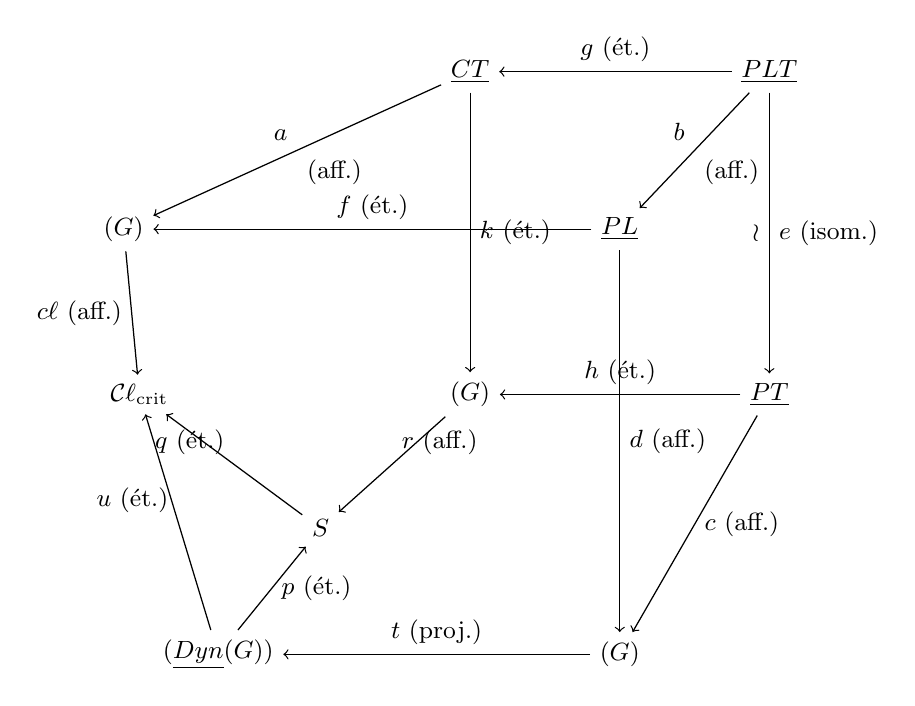
\begin{tikzpicture}[
  >=to,
  every node/.style={font=\small},
  morph/.style={->,line width=.45pt}
]
  \node (CT)     at (5.2,7.2) {\(\underline{CT}\)};
  \node (PLT)    at (9.0,7.2) {\(\underline{PLT}\)};
  \node (Crit)   at (0.8,5.2) {\(\Crit(G)\)};
  \node (PL)     at (7.1,5.2) {\(\underline{PL}\)};
  \node (Cl)     at (1.0,3.1) {\(\mathcal C\ell_{\mathrm{crit}}\)};
  \node (Tor)    at (5.2,3.1) {\(\Tor(G)\)};
  \node (PT)     at (9.0,3.1) {\(\underline{PT}\)};
  \node (S)      at (3.3,1.4) {\(S\)};
  \node (Of)     at (2.0,-.2) {\(\Of(\underline{\operatorname{Dyn}}(G))\)};
  \node (Par)    at (7.1,-.2) {\(\Par(G)\)};

  \draw[morph] (PLT) -- node[above]{\(g\) (ét.)} (CT);
  \draw[morph] (CT) -- node[above left]{\(a\)} node[below right]{(aff.)} (Crit);
  \draw[morph] (PLT) -- node[above left]{\(b\)} node[below right]{(aff.)} (PL);
  \draw[morph] (PL) -- node[above]{\(f\) (ét.)} (Crit);
  \draw[morph] (CT) -- node[right]{\(k\) (ét.)} (Tor);
  \draw[morph] (PLT) -- node[left]{\(\wr\)}
    node[right]{\(e\) (isom.)} (PT);
  \draw[morph] (Crit) -- node[left]{\(c\ell\) (aff.)} (Cl);
  \draw[morph] (PL) -- node[right]{\(d\) (aff.)} (Par);
  \draw[morph] (PT) -- node[above]{\(h\) (ét.)} (Tor);
  \draw[morph] (PT) -- node[right]{\(c\) (aff.)} (Par);
  \draw[morph] (S) -- node[above left]{\(q\) (ét.)} (Cl);
  \draw[morph] (Tor) -- node[above right]{\(r\) (aff.)} (S);
  \draw[morph] (Of) -- node[above left]{\(u\) (ét.)} (Cl);
  \draw[morph] (Of) -- node[right]{\(p\) (ét.)} (S);
  \draw[morph] (Par) -- node[above]{\(t\) (proj.)} (Of);
\end{tikzpicture}
\refstepcounter{figure}
\label{sga3:xxvi:fig:3:15:1}
\par\smallskip
{\small Figure 3.15.1}
\end{figure}
\SGARefTarget{sga3:xxvi:item:3:15}

\begin{sgastatement}{Theorem 3.16 \textup{(cf.\ Figure 3.15.1)}}
\begin{enumerate}[label=\textup{(\roman*)}]
\item Every morphism in the diagram is smooth, surjective, and of finite
presentation.
\item Every morphism except \(t\) is affine; \(t\) is projective.
\item Every morphism is either finite étale or has integral geometric
fibers: \(f,g,h,k,p,q,u\) are finite étale;
\(a,b,c,d,r,c\ell\) have integral geometric fibers; and \(e\) is an
isomorphism.
\item The square \((a,b,f,g)\) is cartesian.
\end{enumerate}
\end{sgastatement}
\SGARefTarget{sga3:xxvi:thm:3:16}

\SGAProof
It is clear from \SGARefLink{sga3:xxvi:proposition:1-6:item:ii}{1.6(ii)} that \(e\) is an isomorphism, and (iv) is
immediate.  The morphism \(a\) is smooth and affine with integral
geometric fibers.  Indeed, after the base change \(\Crit(G)\to S\), this
reduces to the same statement for
\[
 \Tor(L_0)\longrightarrow S,
\]
where \(L_0\) is the universal critical subgroup; \(L_0\) is reductive by
definition, so Exp.\ XXII, \SGARefLink{sga3:xxii:cor:5.8.3}{5.8.3} applies.  By (iv), \(b\) has the same
properties.

The morphism \(d\) is likewise smooth and affine with integral geometric
fibers, by \SGARefLink{sga3:xxvi:cor:1:9}{1.9}; the same is therefore true of
\[
 c=dbe^{-1}.
\]
The morphism \(r\) has these properties by Exp.\ XXII, \SGARefLink{sga3:xxii:cor:5.8.3}{5.8.3}, and
\(c\ell\) by \SGARefLink{sga3:xxvi:item:3:9}{3.10}.

We already know that \(p\) and \(q\) are finite étale and surjective
(\SGARefLink{sga3:xxvi:paragraph:3-1}{3.1} and \SGARefLink{sga3:xxvi:paragraph:3-9}{3.9}).  If \(f\) and \(k\) are finite étale and surjective, then
so is \(g\), by (iv), and so is \(h=kge^{-1}\).  Since the assertions
about \(t\) were proved in \SGARefLink{sga3:xxvi:thm:3:3:item:ii}{3.3(ii)}, it remains only to prove the claim for
\(f\) and \(k\).  We do so for \(k\), the proof for \(f\) being the same.

If \(T\) is a maximal torus of \(G\), let \(\mathcal C\) be the functor of
critical subgroups containing \(T\).  We must show that \(\mathcal C\) is
represented by a finite étale \(S\)-scheme with nonempty fibers.  We may
suppose that \(G\) is split relative to \(T\).  If \(E\) is the set of
vectorial subsets of the root system \(R\), then \(\mathcal C\) is
represented by \(E_S\), by 3.9.
\SGAQED

\begin{sgastatement}{Corollary 3.17}
All the functors in the preceding diagram are representable by
\(S\)-schemes that are smooth over \(S\), and all are affine over \(S\)
except \(\Par(G)\).
\end{sgastatement}
\SGARefTarget{sga3:xxvi:cor:3:17}

\begin{sgastatement}{\SGAInlineRefTarget{sga3:xxvi:remark:3-18}Remark 3.18}
\begin{enumerate}[label=\textup{(\roman*)}]
\item The fact that \(f:PL\to\Crit(G)\) is étale and surjective says that
a subgroup of \(G\) is critical if and only if, locally for the étale
topology, it is a Levi subgroup of a parabolic subgroup.

In general the map \(PL(S)\to\Crit(G)(S)\) need not be surjective: a
critical subgroup \(C\) may fail to arise over \(S\) from a parabolic
subgroup.  For example, a maximal torus need not be contained in a Borel
subgroup, as for a nonsplit form of \(\operatorname{SL}_2\)
\textup{(Exp.\ XX, §5)}.
\item Likewise,
\[
 u:\Of(\underline{\operatorname{Dyn}}(G))
 \longrightarrow\mathcal C\ell_{\mathrm{crit}}
\]
need not be an isomorphism.  Two parabolic subgroups of different types
may have Levi subgroups of the same type.  In a group of type \(A_2\),
for instance, the two types of parabolics whose Levi subgroups have
semisimple rank \(1\) correspond to the two vertices of the diagram,
whereas there is only one type of critical subgroup of rank \(1\).

The analogous example for type \(A_3\) shows that, even over an
algebraically closed field, nonisomorphic parabolic subgroups may have
Levi subgroups of the same type.\footnote{\emph{Editor's note.}
Concretely, in \(\operatorname{GL}_4\), the parabolics
\[
 P=\left\{\begin{pmatrix}
 *&*&*&*\\0&*&*&*\\0&0&*&*\\0&0&0&*
 \end{pmatrix}\right\},
 \qquad
 P'=\left\{\begin{pmatrix}
 *&*&*&*\\0&*&*&*\\0&*&*&*\\0&0&0&*
 \end{pmatrix}\right\}
\]
are not isomorphic (their unipotent radicals are not isomorphic), while
their Levi subgroups
\[
 L=\left\{\begin{pmatrix}
 *&*&0&0\\ *&*&0&0\\0&0&*&0\\0&0&0&*
 \end{pmatrix}\right\},
 \quad
 L'=\left\{\begin{pmatrix}
 *&0&0&0\\0&*&*&0\\0&*&*&0\\0&0&0&*
 \end{pmatrix}\right\}
\]
are conjugate by
\(
\left(\begin{smallmatrix}
0&0&1&0\\0&1&0&0\\1&0&0&0\\0&0&0&1
\end{smallmatrix}\right).
\)}
\end{enumerate}
\end{sgastatement}
\SGARefTarget{sga3:xxvi:rem:3:18}

We end this section with an application to principal bundles.

\begin{sgastatement}{\SGAInlineRefTarget{sga3:xxvi:lemma:3-20}Lemma 3.20}
Let\footnote{\emph{Editor's note.} The numbering of the original is
retained: there is no §3.19.} \(S\) be a scheme, \(G\) an \(S\)-reductive group, \(F\) a principal
homogeneous bundle under \(G\), and \(G_F\) the corresponding twisted form.
Identify \(\underline{\operatorname{Dyn}}(G)\) with
\(\underline{\operatorname{Dyn}}(G_F)\) \textup{(Exp.\ XXIV, \SGARefLink{sga3:xxiv:3.5}{3.5})}.
For every parabolic subgroup \(P\) of \(G\), there is a canonical
isomorphism
\[
 F/P\xrightarrow{\sim}\Par_{t(P)}(G_F).
\]
In particular, the structural group of \(F\) reduces to \(P\) if and only
if \(G_F\) has a parabolic subgroup of type \(t(P)\).
\end{sgastatement}
\SGARefTarget{sga3:xxvi:lemma:3:20}

The proof is exactly the same as that of Exp.\ XXIV, \SGARefLink{sga3:xxiv:proposition:4-2-1}{4.2.1}.

\SGAInlineRefTarget{sga3:xxvi:paragraph:3-21}\paragraph{\SGARefLink{sga3:xxvi:paragraph:3-21}{3.21}.}
If \(S\) is a scheme, \(G\) an \(S\)-reductive group, and
\[
 t\in\Of(\underline{\operatorname{Dyn}}(G))(S),
\]
write \(H^1_t(S,G)\) for the subset of \(H^1(S,G)\) consisting of the
classes of principal \(G\)-bundles \(F\) for which the associated group
\(G_F\) has a parabolic subgroup of type \(t\).  If \(G\) itself has a
parabolic subgroup \(P\) of type \(t\), then \(H^1_t(S,G)\) is precisely
the image of \(H^1(S,P)\) in \(H^1(S,G)\), and hence does not depend on
the chosen \(P\).
\SGARefTarget{sga3:xxvi:item:3:21}

% END inputs/XXVI/tex/components/02_section3.tex

% BEGIN inputs/XXVI/tex/components/03_section4_1_through_4_2_4.tex
\SGASection{4}{Relative position of two parabolic subgroups}
\SGARefTarget{sga3:xxvi:section:4}

\SGASubsection{4.1}{A preliminary result}
\SGARefTarget{sga3:xxvi:subsection:4:1}

\begin{sgastatement}{Lemma 4.1.1}
Let \(k\) be a field, \(G\) a reductive \(k\)-group, and \(P,P'\) two
parabolic subgroups of \(G\).
\begin{enumerate}[label=\textup{(\roman*)}]
\item The intersection \(P\cap P'\) is smooth, has the same reductive
rank as \(G\), and contains a maximal torus \(T\) of \(G\).
\item The set \(R'\) of roots of \(P\cap P'\) relative to \(T\) is a
closed subset of the set \(R\) of roots of \(G\) relative to \(T\).
\end{enumerate}
\end{sgastatement}
\SGARefTarget{sga3:xxvi:lemma:4:1:1}
\footnote{\emph{Editor's note.} Part \textup{(ii)}, which will be useful
in \SGARefLink{sga3:xxvi:proposition:4-5-1}{4.5.1}, was added by the editors.}

\SGAProof
Suppose first that \(k\) is algebraically closed.  Let \(B\) (respectively
\(B'\)) be a Borel subgroup of \(P\) (respectively \(P'\)).  There is an
element \(g\in G(k)\) such that \(\Int(g)B=B'\).  On the other hand, if
\(T_0\) is a maximal torus of \(B\) and \(N=\Norm_G(T_0)\), Bruhat's
theorem (\emph{Bible}, §13.4, Corollary 1 to Theorem 3) gives
\[
 G(k)=B(k)N(k)B(k).
\]
Thus there are \(b,b_1\in B(k)\) and \(n\in N(k)\) such that
\(g=bnb_1\), and hence
\(\Int(b)\Int(n)B=B'\).  Consequently
\[
 P\cap P'\supset B\cap B'
  =\Int(b)\bigl(B\cap\Int(n)B\bigr)
  \supset\Int(b)T_0.
\]

Now let \(k\) be arbitrary.  The preceding result shows that
\(P_{\bar k}\cap P'_{\bar k}\) contains a maximal torus of
\(G_{\bar k}\).  By Exp.\ XXII, \SGARefLink{sga3:xxii:prop:5.4.5}{5.4.5},
\((P\cap P')_{\bar k}\) is smooth along the identity section; since the
base is a field, it is therefore smooth (Exp.\ VI\textsubscript{A},
\SGARefLink{prop:sga3-VIA-1.3.1}{1.3.1}), and so \(P\cap P'\) is smooth.  By Exp.\ VI\textsubscript{A},
\SGARefLink{prop:sga3-VIA-2.3.1}{2.3.1}, the identity component \((P\cap P')^0\) is an open subgroup of
\(P\cap P'\), smooth over \(k\).  Applying Exp.\ XIV, \SGARefLink{sga3:xiv:1.1}{1.1} to it proves
\textup{(i)}.

Finally, the set \(R_P\) (respectively \(R_{P'}\)) of roots of \(P\)
(respectively \(P'\)) relative to \(T\) is closed, and
\[
 R'=R_P\cap R_{P'}.
\]
This proves \textup{(ii)}.
\SGAQED

\begin{sgastatement}{Remark 4.1.2}
One can prove \textup{([BT65], \SGARefLink{sga3:xxvi:subsection:4:5}{4.5})} that \(P\cap P'\) is connected; this
fact will be used in \SGARefLink{sga3:xxvi:proposition:4-5-1}{4.5.1}.
\end{sgastatement}
\SGARefTarget{sga3:xxvi:remark:4:1:2}
\footnote{\emph{Editor's note.} In view of the details added in \SGARefLink{sga3:xxvi:proposition:4-5-1}{4.5.1},
the original wording ``we shall not use this fact'' was changed.}

\begin{sgastatement}{\SGAInlineRefTarget{sga3:xxvi:remark:4-1-3}Remark 4.1.3}
The preceding lemma is false over an arbitrary scheme.  For example, let
\(G\) be a reductive group over an algebraically closed field \(k\), and
let \(B\) be a Borel subgroup of \(G\).  Take \(S=G\) as base and
consider the Borel subgroups \(B_1,B_2\) of \(G_G\), where
\[
 B_1=B_G,\qquad B_2=\Int(g_0)B_1,
\]
and \(g_0\) is the canonical (diagonal) section of \(G_G\).  For every
\(g\in G(k)\), the fiber of \(B_1\cap B_2\) at \(g\) is
\(B\cap\Int(g)B\).  If \(B\ne G\), the dimension of this fiber varies
with \(g\), so \(B_1\cap B_2\) cannot be smooth over \(G\).
\end{sgastatement}
\SGARefTarget{sga3:xxvi:remark:4:1:3}

\SGASubsection{4.2}{Transversal position}
\SGARefTarget{sga3:xxvi:subsection:4:2}

\begin{sgastatement}{\SGAInlineRefTarget{sga3:xxvi:theorem:4-2-1}Theorem 4.2.1}
Let \(S\) be a scheme, \(G\) an \(S\)-reductive group, and \(P,Q\) two
parabolic subgroups of \(G\).  The following conditions on the pair
\((P,Q)\) are equivalent:
\begin{enumerate}[leftmargin=3.2em,labelsep=.7em]
\item[\textup{\SGAInlineRefTarget{sga3:xxvi:theorem:4-2-1:item:i}(i)}]
\(\operatorname{Lie}(P/S)+\operatorname{Lie}(Q/S)
  =\operatorname{Lie}(G/S)\).
\item[\textup{\SGAInlineRefTarget{sga3:xxvi:theorem:4-2-1:item:ii}(ii)}]
The canonical morphism \(P\times_SQ\to G\) is smooth.
\item[\textup{(ii\(^{\prime}\))}]
The canonical morphism \(P\to G/Q\) is smooth.
\item[\textup{\SGAInlineRefTarget{sga3:xxvi:theorem:4-2-1:item:iii}(iii)}]
The canonical morphism \(P\times_SQ\to G\) is open.
\item[\textup{(iii\(^{\prime}\))}]
The canonical morphism \(P\to G/Q\) is open.
\item[\textup{\SGAInlineRefTarget{sga3:xxvi:theorem:4-2-1:item:iv}(iv)}]
The canonical morphism \(P\times_SQ\to G\) is fiberwise dominant.
\item[\textup{(iv\(^{\prime}\))}]
The canonical morphism \(P\to G/Q\) is fiberwise dominant.
\item[\textup{\SGAInlineRefTarget{sga3:xxvi:theorem:4-2-1:item:v}(v)}]
For every \(s\in S\), the group \(P_s\cap Q_s\) has minimum dimension,
that is,
\[
 \dim(P_s\cap Q_s)=\dim P_s+\dim Q_s-\dim G_s.
\]
\item[\textup{\SGAInlineRefTarget{sga3:xxvi:theorem:4-2-1:item:vi}(vi)}]
There is an étale covering family \(\{S_i\to S\}\) and, for every \(i\),
a Borel subgroup \(B_i\) of \(P_{S_i}\) and a Borel subgroup \(B'_i\)
of \(Q_{S_i}\), such that \(B_i\cap B'_i\) is a maximal torus of
\(G_{S_i}\).
\item[\textup{\SGAInlineRefTarget{sga3:xxvi:theorem:4-2-1:item:vii}(vii)}]
There is an étale covering family \(\{S_i\to S\}\) and, for every \(i\),
a splitting \((T_i,\ldots,R_i)\) of \(G_{S_i}\) and a system
\(R_i^+\) of positive roots of \(R_i\), such that \(P_{S_i}\)
(respectively \(Q_{S_i}\)) is the subgroup of type \textup{(R)} of
\(G_{S_i}\) containing \(T_i\) and defined by a subset \(R_i^{(1)}\)
(respectively \(R_i^{(2)}\)) of \(R_i\) containing \(R_i^+\)
(respectively \(-R_i^+\)); see Exp.\ XXII, \SGARefLink{sga3:xxii:def:5.4.2}{5.4.2} and 5.2.1.
\end{enumerate}
\end{sgastatement}
\SGARefTarget{sga3:xxvi:theorem:4:2:1}

\SGAProof
We prove the theorem according to the following logical diagram:
\[
\begin{tikzcd}[column sep=large,row sep=large]
 \textup{(i)} \arrow[d,Rightarrow] &
 \textup{(vii)} \arrow[l,Rightarrow] &
 \textup{(vi)} \arrow[l,Rightarrow] \\
 \textup{(ii\(^{\prime}\))} \arrow[d,Rightarrow] \arrow[r,Rightarrow] &
 \textup{(iii\(^{\prime}\))} \arrow[r,Rightarrow] &
 \textup{(iv\(^{\prime}\))} \arrow[r,Rightarrow] &
 \textup{(v)} \arrow[ul,Rightarrow] \\
 \textup{(ii)} \arrow[r,Rightarrow] &
 \textup{(iii)} \arrow[r,Rightarrow] &
 \textup{(iv)} \arrow[ur,Rightarrow] &
 {} .
\end{tikzcd}
\]

The implications \textup{\SGARefLink{sga3:xxvi:theorem:4-2-1:item:ii}{(ii)}} \(\Rightarrow\) \textup{\SGARefLink{sga3:xxvi:theorem:4-2-1:item:iii}{(iii)}} and
\textup{(ii\(^{\prime}\))} \(\Rightarrow\)
\textup{(iii\(^{\prime}\))} are immediate.  If \textup{\SGARefLink{sga3:xxvi:theorem:4-2-1:item:iii}{(iii)}} holds,
the set-theoretic image of \(P\times_SQ\to G\) is an open subset of
\(G\) containing the identity section.  Since the fibers of \(G\) are
connected, this image is dense in every fiber; thus \textup{\SGARefLink{sga3:xxvi:theorem:4-2-1:item:iv}{(iv)}}
holds.  The implication
\textup{(iii\(^{\prime}\))} \(\Rightarrow\)
\textup{(iv\(^{\prime}\))} is identical.

Condition \textup{(ii\(^{\prime}\))} implies \textup{\SGARefLink{sga3:xxvi:theorem:4-2-1:item:ii}{(ii)}}, by the
cartesian diagram
\[
\begin{tikzcd}[column sep=large,row sep=large]
 P\times_SQ \arrow[r] \arrow[d,"\operatorname{pr}_1"'] & G \arrow[d]\\
 P \arrow[r] & G/Q .
\end{tikzcd}
\]
On the other hand, \textup{(iv)} or \textup{(iv\(^{\prime}\))}
implies \textup{(v)} by dimension theory (EGA
IV\textsubscript{2}, 5.6.6).  Indeed, one may assume
\(S=\operatorname{Spec}(k)\), with \(k\) algebraically closed; every
nonempty fiber of the morphism in \textup{\SGARefLink{sga3:xxvi:theorem:4-2-1:item:iv}{(iv)}} at a point of \(G(k)\),
or of the morphism in \textup{(iv\(^{\prime}\))} at a point of
\((G/Q)(k)\), is isomorphic to \(P\cap Q\).

The implication \textup{\SGARefLink{sga3:xxvi:theorem:4-2-1:item:vi}{(vi)}} \(\Rightarrow\) \textup{\SGARefLink{sga3:xxvi:theorem:4-2-1:item:vii}{(vii)}} follows
from Exp.\ XXII, \SGARefLink{sga3:xxii:prop:5.5.1}{5.5.1} \textup{\SGARefLink{sga3:xxvi:theorem:4-2-1:item:iv}{(iv)}} and \SGARefLink{sga3:xxii:prop:5.9.2}{5.9.2}.  Condition
\textup{\SGARefLink{sga3:xxvi:theorem:4-2-1:item:vii}{(vii)}} implies \textup{\SGARefLink{sga3:xxvi:theorem:4-2-1:item:i}{(i)}}, because the latter may be checked
fpqc-locally.  Under \textup{\SGARefLink{sga3:xxvi:theorem:4-2-1:item:vii}{(vii)}} we may therefore suppose that
\(G\) is split, \(P\supset B_{R^+}\), and
\(Q\supset B_{-R^+}\); then already
\[
 \operatorname{Lie}(B_{R^+})+\operatorname{Lie}(B_{-R^+})
 =\operatorname{Lie}(G).
\]

Let us prove that \textup{\SGARefLink{sga3:xxvi:theorem:4-2-1:item:i}{(i)}} implies
\textup{(ii\(^{\prime}\))}.  Let \(u:P\to G/Q\) be the canonical
morphism.  Smoothness can be checked on geometric fibers, since both
\(P\) and \(G/Q\) are smooth over \(S\); hence we may suppose that
\(S\) is the spectrum of an algebraically closed field.  The morphism
\(u\) is compatible with the evident action of \(P\):
\(u(pp')=p\,u(p')\).  A translation argument (compare the proof of
Exp.\ VI\textsubscript{B}, 1.3) therefore reduces smoothness to the
point \(e\in P(k)\).  By SGA 1, II, 4.7, it is enough that the tangent
map at \(e\) be surjective.  This map is naturally identified with
\[
 \operatorname{Lie}(P)\longrightarrow
 \operatorname{Lie}(G)/\operatorname{Lie}(Q),
\]
which is surjective under \textup{\SGARefLink{sga3:xxvi:theorem:4-2-1:item:i}{(i)}}.

It remains to prove \textup{\SGARefLink{sga3:xxvi:theorem:4-2-1:item:v}{(v)}} \(\Rightarrow\) \textup{\SGARefLink{sga3:xxvi:theorem:4-2-1:item:vi}{(vi)}}.
Suppose first that \(S\) is the spectrum of an algebraically closed
field.  By \SGARefLink{sga3:xxvi:lemma:4:1:1}{4.1.1} there is a maximal torus \(T\) contained in \(P\) and
\(Q\).  Let \(R\), \(R_1\), and \(R_2\) be the respective sets of roots
of \(G\), \(P\), and \(Q\) relative to \(T\).  By Exp.\ XXII, \SGARefLink{sga3:xxii:lem:5.4.4}{5.4.4} and
\SGARefLink{sga3:xxii:prop:5.4.5}{5.4.5},
\[
\begin{aligned}
 \dim G&=\dim T+\operatorname{Card}(R),&
 \dim P&=\dim T+\operatorname{Card}(R_1),\\
 \dim Q&=\dim T+\operatorname{Card}(R_2),&
 \dim(P\cap Q)&=\dim T+\operatorname{Card}(R_1\cap R_2).
\end{aligned}
\]
Condition \textup{\SGARefLink{sga3:xxvi:theorem:4-2-1:item:v}{(v)}} is therefore equivalent to
\[
 \operatorname{Card}(R_1\cap R_2)
 =\operatorname{Card}(R_1)+\operatorname{Card}(R_2)
  -\operatorname{Card}(R),
\]
that is, to \(R_1\cup R_2=R\).  By Exp.\ XXII, \SGARefLink{sga3:xxii:prop:5.9.2}{5.9.2} and \SGARefLink{sga3:xxii:prop:5.4.5}{5.4.5}, it is
enough to prove that \(R_1\cap(-R_2)\) contains a system of positive
roots of \(R\).  We are thus reduced to the following lemma.

\begin{sgastatement}{Lemma 4.2.2}
Let \(R\) be a ``root system''---for example, the set of roots of a root
datum in the sense of Exposé XXI.  Let \(R_1,R_2\) be two closed subsets
of \(R\), each containing a system of positive roots.  If
\(R_1\cup R_2=R\), then \(R_1\cap(-R_2)\) contains a system of positive
roots.
\end{sgastatement}
\SGARefTarget{sga3:xxvi:lemma:4:2:2}

Indeed, \(R_3=R_1\cap(-R_2)\) is closed, so by Exp.\ XXI, \SGARefLink{sga3:XXI:3.3.6}{3.3.6} it is
enough to show that \(R_3\cup(-R_3)=R\).  Now
\[
 R_1\cup(-R_1)=R=R_2\cup(-R_2),
\]
and the conclusion follows from the following elementary fact.  If
\(A,A',B,B'\) are four subsets of a set \(E\), and
\[
 A\cup A'=B\cup B'=A\cup B=A'\cup B'=E,
\]
then
\[
 (A\cap B')\cup(A'\cap B)=E.
\]

This proves \textup{\SGARefLink{sga3:xxvi:theorem:4-2-1:item:v}{(v)}} \(\Rightarrow\) \textup{\SGARefLink{sga3:xxvi:theorem:4-2-1:item:vi}{(vi)}} over the
spectrum of an algebraically closed field.  Return now to the general
case and suppose \textup{\SGARefLink{sga3:xxvi:theorem:4-2-1:item:v}{(v)}} holds.  Let \(s\in S\).  By the preceding
argument, there is a Borel subgroup \(\bar B\) of \(P_{\bar s}\) and a
Borel subgroup \(\bar B'\) of \(Q_{\bar s}\) such that
\(\bar B\cap\bar B'\) is a maximal torus of \(G_{\bar s}\).

The \(S\)-scheme
\[
 \Bor(P)\simeq\Bor\bigl(P/\rad^u(P)\bigr)
\]
of Borel subgroups of \(P\) is smooth.  Applying ``Hensel's lemma''
(Exp.\ XI, \SGARefLink{sga3:xi:proposition:1:10}{1.10}) and working étale-locally around \(s\), we may suppose
that there is a Borel subgroup \(B\) of \(P\) specializing to
\(\bar B\).  Similarly, there is a Borel subgroup \(B'\) of \(Q\)
specializing to \(\bar B'\).  Since
\(\bar B\cap\bar B'\) is a maximal torus of \(G_{\bar s}\), some open
neighborhood \(U\) of \(s\) has the property that
\(B_U\cap B'_U\) is a maximal torus of \(G_U\)
(Exp.\ XXII, \SGARefLink{sga3:xxii:cor:5.9.4}{5.9.4}).  This proves \textup{\SGARefLink{sga3:xxvi:theorem:4-2-1:item:vi}{(vi)}}.
\SGAQED

\begin{sgastatement}{Definition 4.2.3}
A pair \((P,Q)\) satisfying the equivalent conditions
\textup{\SGARefLink{sga3:xxvi:theorem:4-2-1:item:i}{(i)}}--\textup{\SGARefLink{sga3:xxvi:theorem:4-2-1:item:vii}{(vii)}} of \SGARefLink{sga3:xxvi:theorem:4-2-1}{Theorem 4.2.1} is said to be in
\emph{transversal position}.  One also says that \(P\) is in
transversal position relative to \(Q\), or, by an abuse of language,
that \(P\) and \(Q\) are in (mutual) transversal position.
\end{sgastatement}
\SGARefTarget{sga3:xxvi:def:4:2:3}

In view of \textup{\SGARefLink{sga3:xxvi:theorem:4-2-1:item:vi}{(vi)}}, this definition agrees, for Borel subgroups,
with that of Exp.\ XXII, \SGARefLink{sga3:xxii:def:5.9.1}{5.9.1}.

\begin{sgastatement}{\SGAInlineRefTarget{sga3:xxvi:corollary:4-2-4}Corollary 4.2.4}
Let \(S\) be a scheme, \(G\) an \(S\)-reductive group, and \(P,Q\) two
parabolic subgroups of \(G\).
\begin{enumerate}[label=\textup{(\roman*)}]
\item The pair \((P,Q)\) is in transversal position if and only if, for
every \(s\in S\), the pair \((P_{\bar s},Q_{\bar s})\) is in transversal
position.  If \(S'\to S\) is surjective and
\((P_{S'},Q_{S'})\) is in transversal position, then so is \((P,Q)\).
\item There is an open subscheme \(U\subset S\) with the following
property: a morphism \(S'\to S\) factors through \(U\) if and only if
\((P_{S'},Q_{S'})\) is in transversal position.
\item Consider the subfunctors
\[
 \Gen(G)\subset\Par(G)\times_S\Par(G),\qquad
 \Gen(/Q)\subset\Par(G),\qquad
 \Gen(P/Q)\subset G,
\]
defined as follows.  For \(S'\to S\), the set \(\Gen(G)(S')\) consists
of pairs of parabolic subgroups of \(G_{S'}\) in transversal position;
\(\Gen(/Q)(S')\) consists of parabolic subgroups of \(G_{S'}\) in
transversal position relative to \(Q_{S'}\); and \(\Gen(P/Q)(S')\)
consists of the \(g\in G(S')\) such that \(\Int(g)P_{S'}\) is in
transversal position relative to \(Q_{S'}\).

Each of these functors is represented by an open subscheme,
universally schematically dense over \(S\), of the corresponding
\(S\)-scheme
\[
 \Par(G)\times_S\Par(G),\qquad\Par(G),\qquad G,
\]
respectively.
\end{enumerate}
\end{sgastatement}
\SGARefTarget{sga3:xxvi:cor:4:2:4}
\footnote{\emph{Editor's note.} The original expression ``relatively
dense'' was replaced by ``universally schematically dense over \(S\)'';
compare EGA IV\textsubscript{3}, Definition 11.10.8.}

Assertion \textup{\SGARefLink{sga3:xxvi:theorem:4-2-1:item:i}{(i)}} follows immediately from condition
\SGARefLink{sga3:xxvi:theorem:4-2-1}{4.2.1}\textup{\SGARefLink{sga3:xxvi:theorem:4-2-1:item:i}{(i)}}.  For \textup{\SGARefLink{sga3:xxvi:theorem:4-2-1:item:ii}{(ii)}}, take
\[
 U=S-\operatorname{Supp}(\operatorname{Coker}u),
\]
where
\[
 u:\operatorname{Lie}(P)\oplus\operatorname{Lie}(Q)
   \longrightarrow\operatorname{Lie}(G)
\]
is the canonical morphism.\footnote{\emph{Editor's note.} The second
summand, printed as \(\operatorname{Lie}(G)\), has been corrected to
\(\operatorname{Lie}(Q)\); this is the map used in \SGARefLink{sga3:xxvi:theorem:4-2-1}{Theorem
4.2.1}\textup{\SGARefLink{sga3:xxvi:theorem:4-2-1:item:i}{(i)}}.}

There are cartesian diagrams
\[
\begin{tikzcd}[column sep=large,row sep=large]
 G \arrow[r,"f"] & \Par(G)\\
 \Gen(P/Q) \arrow[u,hook] \arrow[r] & \Gen(/Q)\arrow[u,hook]
\end{tikzcd}
\qquad
\begin{tikzcd}[column sep=large,row sep=large]
 \Par(G) \arrow[r,"f'"] & \Par(G)\times_S\Par(G)\\
 \Gen(/Q) \arrow[u,hook] \arrow[r] & \Gen(G)\arrow[u,hook],
\end{tikzcd}
\]
where \(f(g)=\Int(g)P\) and \(f'(R)=(R,Q)\).  It therefore suffices to
prove \textup{\SGARefLink{sga3:xxvi:theorem:4-2-1:item:iii}{(iii)}} for \(\Gen(G)\).

Let \(P_0\) be the canonical parabolic subgroup of
\(G_{\Par(G)}\), and set
\[
 X=\Par(G)\times_S\Par(G),\qquad
 P=\operatorname{pr}_1^*(P_0),\qquad
 Q=\operatorname{pr}_2^*(P_0).
\]
Applying \textup{\SGARefLink{sga3:xxvi:theorem:4-2-1:item:ii}{(ii)}} to the parabolic subgroups \(P,Q\) of \(G_X\)
constructs an open subscheme \(U\subset X\), which is immediately
identified with \(\Gen(G)\).  The density assertion may be checked on
geometric fibers,\footnote{\emph{Editor's note.} Compare EGA
IV\textsubscript{3}, 11.10.10.} so assume
\(S=\operatorname{Spec}(k)\), where \(k\) is algebraically closed.
Since \(\Par(G)\) is smooth, it is enough to show that \(\Gen(G)\)
meets every irreducible component of
\(\Par(G)\times_S\Par(G)\).  By \SGARefLink{sga3:xxvi:item:3:2}{3.3}, this amounts to the following:
given \(t,t'\in\Of(\underline{\operatorname{Dyn}}(G))(S)\), find a pair
\((P,P')\) in transversal position such that \(t(P)=t\) and
\(t(P')=t'\).

Choose Borel subgroups \(B,B'\) of \(G\) such that \(B\cap B'\) is a
maximal torus (split \(G\) and apply Exp.\ XXII, \SGARefLink{sga3:xxii:prop:5.9.2}{5.9.2}).  By \SGARefLink{sga3:xxvi:lemma:3:8}{3.8} there
are parabolic subgroups \(P\supset B\) and \(P'\supset B'\) with
\(t(P)=t\) and \(t(P')=t'\).  They have the required types and are in
transversal position by \SGARefLink{sga3:xxvi:theorem:4-2-1}{4.2.1}\textup{\SGARefLink{sga3:xxvi:theorem:4-2-1:item:vi}{(vi)}}.
\SGAQED

% END inputs/XXVI/tex/components/03_section4_1_through_4_2_4.tex

% BEGIN inputs/XXVI/tex/components/04_section4_2_5_through_4_2_7.tex
\begin{sgastatement}{\SGAInlineRefTarget{sga3:xxvi:corollary:4-2-5}Corollary 4.2.5}
Let \(S\) be a scheme, \(G\) an \(S\)-reductive group, and \(P,Q\) two
parabolic subgroups of \(G\), with \((P,Q)\) in transversal position.
\begin{enumerate}[label=\textup{(\roman*)}]
\item Let \(P',Q'\) be parabolic subgroups of \(G\) of the same types as
\(P,Q\), respectively.  The pair \((P',Q')\) is in transversal position
if and only if, étale-locally, it is conjugate to \((P,Q)\).
\textup{(In §5 we shall see that the étale topology can be replaced by
the Zariski topology.)}
\item The canonical morphism \(P\times_SQ\to G\) induces a smooth
surjective morphism
\[
 P\times_SQ\longrightarrow\Gen(Q/P)
\]
and an isomorphism
\[
 (P\times_SQ)/(P\cap Q)\xrightarrow{\sim}\Gen(Q/P),
\]
where \(R=P\cap Q\) acts on \(P\times_SQ\) by
\[
 (p,q)r=(pr,r^{-1}q).
\]
\item The canonical morphism
\[
 P\longrightarrow\Par_{t(Q)}(G),\qquad p\longmapsto\Int(p)Q,
\]
induces a smooth surjective morphism
\[
 P\longrightarrow\Gen(/P)\cap\Par_{t(Q)}(G)
\]
and an isomorphism
\[
 P/(P\cap Q)\xrightarrow{\sim}
 \Gen(/P)\cap\Par_{t(Q)}(G).
\]
\item The canonical morphism
\[
 G\longrightarrow\Par_{t(P)}(G)\times_S\Par_{t(Q)}(G),\qquad
 g\longmapsto\bigl(\Int(g)P,\Int(g)Q\bigr),
\]
induces a smooth surjective morphism
\[
 G\longrightarrow
 \Gen(G)\cap
 \bigl(\Par_{t(P)}(G)\times_S\Par_{t(Q)}(G)\bigr)
\]
and an isomorphism
\[
 G/(P\cap Q)\xrightarrow{\sim}
 \Gen(G)\cap
 \bigl(\Par_{t(P)}(G)\times_S\Par_{t(Q)}(G)\bigr).
\]
\end{enumerate}
\end{sgastatement}
\SGARefTarget{sga3:xxvi:cor:4:2:5}

\SGAProof
Let us prove \textup{(i)}.  The stated condition is plainly sufficient.
Conversely, suppose \((P',Q')\) is in transversal position.  Since
\(P\) and \(P'\) are conjugate étale-locally, we may assume \(P=P'\).
It is then enough to show that two parabolic subgroups \(Q,Q'\), of the
same type and both in transversal position relative to \(P\), are
étale-locally conjugate by a section of \(P\).

By \SGARefLink{sga3:xxvi:theorem:4-2-1}{4.2.1}\textup{\SGARefLink{sga3:xxvi:theorem:4-2-1:item:vi}{(vi)}}, after another étale localization there are Borel
subgroups \(B,B'\subset P\), \(B_1\subset Q\), and \(B'_1\subset Q'\)
such that
\[
 B\cap B_1=T,\qquad B'\cap B'_1=T'
\]
are maximal tori of \(G\).  The Killing pairs \((B,T)\) and
\((B',T')\) of \(P\) are étale-locally conjugate in \(P\) (\SGARefLink{sga3:xxvi:lemma:1:16}{1.16}).
We may therefore assume \(B=B'\) and \(T=T'\).  Then
\(B_1=B'_1\) by Exp.\ XXII, \SGARefLink{sga3:xxii:prop:5.9.2}{5.9.2}, and hence \(Q=Q'\) by \SGARefLink{sga3:xxvi:lemma:3:8}{3.8}.

Parts \textup{(ii)}, \textup{(iii)}, and \textup{(iv)} are proved in
parallel.  We prove \textup{(ii)}.  Let \(g\in\Gen(Q/P)(S)\); thus
\(g\in G(S)\) and \(\Int(g)Q\) is in transversal position relative to
\(P\).  The preceding argument shows that \(Q\) and \(\Int(g)Q\) are,
étale-locally, conjugate by a section of \(P\).  Working locally for
this topology, choose \(p\in P(S)\) such that
\(\Int(g)Q=\Int(p)Q\).  Then
\[
 p^{-1}g\in\Norm_G(Q)(S)=Q(S),
\]
so \(g=pq\) for some \(q\in Q(S)\).  Thus the morphism in
\textup{\SGARefLink{sga3:xxvi:theorem:4-2-1:item:ii}{(ii)}} is an étale covering.  Comparing with
\SGARefLink{sga3:xxvi:theorem:4-2-1}{4.2.1}\textup{\SGARefLink{sga3:xxvi:theorem:4-2-1:item:ii}{(ii)}}, it is smooth and surjective.

Finally, the equivalence relation on \(P\times_SQ\) defined by
\(P\times_SQ\to G\) is exactly the relation associated with the action
of \(R=P\cap Q\),
\[
 (p,q)r=(pr,r^{-1}q).
\]
This proves the quotient assertion, since a smooth surjective morphism
is, in particular, an effective epimorphism.
\SGAQED

\begin{sgastatement}{Remark 4.2.6}
If \(P,Q\) are in transversal position, the open subset \(\Gen(Q/P)\)
of \(G\) will often be denoted \(P\cdot Q\); this notation is justified
by \SGARefLink{sga3:xxvi:corollary:4-2-5}{4.2.5}\textup{(ii)}.
\end{sgastatement}
\SGARefTarget{sga3:xxvi:remark:4:2:6}

\begin{sgastatement}{\SGAInlineRefTarget{sga3:xxvi:proposition:4-2-7}Proposition 4.2.7}
Let \(S\) be a scheme, \(G\) an \(S\)-reductive group, and \(P,Q\) two
parabolic subgroups of \(G\), with \((P,Q)\) in transversal position.
\begin{enumerate}[label=\textup{(\roman*)}]
\item The group \(P\cap Q\) is smooth over \(S\) (and in fact has
connected fibers by \SGARefLink{sga3:xxvi:remark:4:1:2}{4.1.2}).  Its identity component
\((P\cap Q)^0\) \textup{(Exp.\ VI\textsubscript{B}, \SGARefLink{thm:sga3-VIB-3.10}{3.10})} is a
subgroup of type \textup{(RC)} of \(G\)
\textup{(Exp.\ XXII, \SGARefLink{sga3:xxii:def:5.11.1}{5.11.1})}, and its unipotent radical
\textup{(loc.\ cit., 5.11.4)} decomposes as the direct product
\[
 \rad^u\bigl((P\cap Q)^0\bigr)
 =
 \bigl(\rad^u(P)\cap Q\bigr)
 \times_S
 \bigl(P\cap\rad^u(Q)\bigr).
\]
\item If \(S\) is affine, then
\[
 H^1\bigl(S,\rad^u((P\cap Q)^0)\bigr)=0.
\]
If \(S\) is semilocal, \(P\cap Q\) contains a maximal torus of \(G\).
\end{enumerate}
\end{sgastatement}
\SGARefTarget{sga3:xxvi:prop:4:2:7}

\SGAProof
The group \(P\cap Q\) is smooth by \SGARefLink{sga3:xxvi:theorem:4-2-1}{4.2.1}\textup{\SGARefLink{sga3:xxvi:theorem:4-2-1:item:ii}{(ii)}} and the
cartesian diagram
\[
\begin{tikzcd}[column sep=large,row sep=large]
 P\times_SQ \arrow[r] & G\\
 P\cap Q \arrow[u] \arrow[r] & S\arrow[u]
\end{tikzcd}.
\]

The remaining assertions about \((P\cap Q)^0\) may be checked
étale-locally.  By \SGARefLink{sga3:xxvi:theorem:4-2-1}{4.2.1}\textup{\SGARefLink{sga3:xxvi:theorem:4-2-1:item:vii}{(vii)}}, choose a splitting
\((G,T,M,R)\) of \(G\) such that \(P,Q\) contain \(T\) and are defined
by subsets \(R_1,R_2\) of \(R\), where \(R_1\) contains a system
\(R^+\) of positive roots and \(R_2\) contains the opposite system
\(R^-\).  Let \(\Delta\) be the set of simple roots of \(R^+\), and put
\[
 A_1=\Delta\cap(-R_1),\qquad
 A_2=\Delta\cap R_2,\qquad
 A=A_1\cap A_2.
\]
By \SGARefLink{sga3:xxvi:prop:1:3}{1.4}\textup{(v)} and \SGARefLink{sga3:xxvi:proposition:1-12}{1.12},
\[
\begin{aligned}
 R_1&=R^+\cup\bigl(R^-\cap(-\mathbb N A_1)\bigr),&
 R_2&=\bigl(R^+\cap\mathbb N A_2\bigr)\cup R^-,\\
 \rad^u(P)&=
   \prod_{\substack{\alpha\in R_1\\\alpha\notin-R_1}}U_\alpha,&
 \rad^u(Q)&=
   \prod_{\substack{\alpha\in R_2\\\alpha\notin-R_2}}U_\alpha.
\end{aligned}
\]
Exp.\ XXII, \SGARefLink{sga3:xxii:cor:5.6.7}{5.6.7} therefore gives
\[
\begin{aligned}
 \rad^u(P)\cap Q
  &=
  \prod_{\substack{\alpha\in R_1\cap R_2\\\alpha\notin-R_1}}U_\alpha
  =\prod_{\alpha\in K_2}U_\alpha,\\
 \rad^u(Q)\cap P
  &=
  \prod_{\substack{\alpha\in R_1\cap R_2\\\alpha\notin-R_2}}U_\alpha
  =\prod_{\alpha\in K_1}U_\alpha,
\end{aligned}
\]
where \(K_2\) consists of the positive roots that are linear
combinations of elements of \(A_2\), but not of elements of \(A\), and
\(K_1\) consists of the negative roots that are linear combinations of
elements of \(A_1\), but not of elements of \(A\).  If
\(\alpha\in K_2\) and \(\beta\in K_1\), then \(\alpha+\beta\) is neither
a root nor zero.  Hence the two groups displayed above commute.

By Exp.\ XXII, \SGARefLink{sga3:xxii:prop:5.4.5}{5.4.5}, the group
\[
 H=(P\cap Q)^0
\]
is defined by the set of roots
\[
 R_1\cap R_2
 =
 \bigl(R^+\cap\mathbb N A_2\bigr)
 \cup
 \bigl(R^-\cap(-\mathbb N A_1)\bigr).
\]
This set is closed, so \(H\) is of type \textup{(RC)} by definition
(Exp.\ XXII, \SGARefLink{sga3:xxii:def:5.11.1}{5.11.1}).  By loc.\ cit., \SGARefLink{sga3:xxii:lem:5.11.3}{5.11.3} and \SGARefLink{sga3:xxii:prop:5.11.4}{5.11.4},
\[
 \rad^u(H)=\prod_{\alpha\in K}U_\alpha,
\]
where \(K\) consists of the \(\alpha\in R_1\cap R_2\) such that
\(\alpha\notin-(R_1\cap R_2)\).  The symmetric part of
\(R_1\cap R_2\) is \(R\cap\mathbb ZA\), and therefore
\(K=K_1\cup K_2\).  This proves \textup{(i)}.

The first assertion of \textup{(ii)} follows from \textup{(i)} and
\SGARefLink{sga3:xxvi:cor:2:10}{2.10}.  For the second, the reductive group
\[
 (P\cap Q)^0/\rad^u((P\cap Q)^0)
\]
has a maximal torus \(\bar T\) when the base is semilocal.  The inverse
image \(N\) of \(\bar T\) in \((P\cap Q)^0\) is a subgroup of type
\textup{(R)} of \(G\), with solvable fibers, and
\[
 N^u=\rad^u((P\cap Q)^0)
\]
(Exp.\ XXII, \SGARefLink{sga3:xxii:prop:5.6.9}{5.6.9}).  The scheme of maximal tori of \(N\) is a
principal homogeneous bundle under \(N^u\) (loc.\ cit., \SGARefLink{sga3:xxii:cor:5.6.13}{5.6.13}), and
therefore has a section because \(H^1(S,N^u)=0\).
\SGAQED

% END inputs/XXVI/tex/components/04_section4_2_5_through_4_2_7.tex

% BEGIN inputs/XXVI/tex/components/05_section4_3.tex
\SGASubsection{4.3}{Opposite parabolic subgroups}
\SGARefTarget{sga3:xxvi:subsection:4:3}

\SGAInlineRefTarget{sga3:xxvi:paragraph:4-3-1}\paragraph{\SGARefLink{sga3:xxvi:paragraph:4-3-1}{4.3.1}.}
Let \(G\) be an \(S\)-reductive group.  Exp.\ XXIV, \SGARefLink{sga3:xxiv:proposition:3-16-6}{3.16.6} defines a
canonical ``outer automorphism'' \(s_G\) of \(G\), of order at most
\(2\).\footnote{\emph{Editor's note.} ``Of order \(2\)'' was replaced
by ``of order at most \(2\)'', since \(s_G\) may be trivial, for example
when \(G\) has type \(A_1,B_n,C_n,\ldots\).}  It induces a canonical
automorphism, again of order at most \(2\), of
\(\underline{\operatorname{Dyn}}(G)\), and hence of
\(\Of(\underline{\operatorname{Dyn}}(G))\).  We denote all of these
automorphisms by \(s_G\), or simply by \(s\).  Two types of parabolic
subgroups
\[
 t,t'\in\Of(\underline{\operatorname{Dyn}}(G))(S)
\]
are said to be \emph{opposite} if \(t=s_G(t')\).
\SGARefTarget{sga3:xxvi:item:4:3:1}

\begin{sgastatement}{Theorem 4.3.2}
Let \(S\) be a scheme, \(G\) an \(S\)-reductive group, and \(P\) a
parabolic subgroup of \(G\).

\textup{(a)} If \(L\) is a Levi subgroup of \(P\), there is a unique
parabolic subgroup \(P'\) of \(G\) such that \(P\cap P'=L\).

\textup{(b)} For every parabolic subgroup \(Q\) of \(G\), the following
conditions are equivalent:
\begin{enumerate}[leftmargin=3.2em,labelsep=.7em]
\item[\textup{\SGAInlineRefTarget{sga3:xxvi:item:4:3:1:item:i}(i)}]
For every \(s\in S\), the identity component
\(\bigl((P\cap Q)_{\bar s}\bigr)^0\), which is smooth by \SGARefLink{sga3:xxvi:lemma:4:1:1}{4.1.1}, is
reductive.
\item[\textup{\SGAInlineRefTarget{sga3:xxvi:item:4:3:1:item:ii}(ii)}]
The group \(P\cap Q\) is a Levi subgroup of both \(P\) and \(Q\).
\item[\textup{\SGAInlineRefTarget{sga3:xxvi:item:4:3:1:item:iii}(iii)}]
The groups \(P,Q\) have opposite types and the pair \((P,Q)\) is in
transversal position.
\item[\textup{\SGAInlineRefTarget{sga3:xxvi:item:4:3:1:item:iv}(iv)}]
The groups \(P,Q\) have opposite types and
\(\rad^u(P)\cap Q=e\).
\item[\textup{\SGAInlineRefTarget{sga3:xxvi:item:4:3:1:item:v}(v)}]
\[
 \rad^u(P)\cap Q=\rad^u(Q)\cap P=e.
\]
\item[\textup{\SGAInlineRefTarget{sga3:xxvi:item:4:3:1:item:vi}(vi)}]
The canonical morphism \(\rad^u(P)\times_SQ\to G\) is an open immersion.
\item[\textup{(vi\(^{\prime}\))}]
The canonical morphism \(\rad^u(P)\to G/Q\) is an open immersion.
\item[\textup{\SGAInlineRefTarget{sga3:xxvi:item:4:3:1:item:vii}(vii)}]
There is an étale covering family \(\{S_i\to S\}\) and, for every \(i\),
a splitting \((T_i,M_i,R_i)\) of \(G_{S_i}\) and a subset
\(R_i^{(1)}\subset R_i\), such that \(P_{S_i}\) is the subgroup of type
\textup{(R)} containing \(T_i\) and defined by \(R_i^{(1)}\), while
\(Q_{S_i}\) is the subgroup defined by
\[
 R_i^{(2)}=-R_i^{(1)}.
\]
\end{enumerate}
\end{sgastatement}
\SGARefTarget{sga3:xxvi:theorem:4:3:2}

\SGAProof
We first prove part \textup{(b)}.  Conditions \textup{\SGARefLink{sga3:xxvi:theorem:4-2-1:item:iii}{(iii)}} and
\textup{\SGARefLink{sga3:xxvi:theorem:4-2-1:item:vii}{(vii)}} are equivalent by \SGARefLink{sga3:xxvi:theorem:4-2-1}{4.2.1}\textup{\SGARefLink{sga3:xxvi:theorem:4-2-1:item:vii}{(vii)}} and the
definition of \(s_G\) in the split case (Exp.\ XXIV,
\SGARefLink{sga3:xxiv:proposition:3-16-2}{3.16.2}\textup{\SGARefLink{sga3:xxiv:proposition:3-16-2:item:iv}{(iv)}}).  Plainly \textup{\SGARefLink{sga3:xxiv:proposition:3-16-2:item:ii}{(ii)}} implies \textup{\SGARefLink{sga3:xxiv:proposition:3-16-2:item:i}{(i)}}, and
\textup{(vi\(^{\prime}\))} implies \textup{\SGARefLink{sga3:xxvi:theorem:4-2-1:item:vi}{(vi)}} by base change along
\(G\to G/Q\).

Suppose now that \textup{\SGARefLink{sga3:xxvi:item:4:3:1:item:vii}{(vii)}} holds.  Since every assertion to be
proved is étale-local, assume that \(G=(G,T,M,R)\) is split, that \(P\)
is defined by \(R'\subset R\), and that \(Q\) is defined by \(-R'\).
Let \(L\) be the subgroup of type \textup{(R)} containing \(T\) and
defined by \(R'\cap(-R')\).  By Exp.\ XXII, \SGARefLink{sga3:xxii:lem:5.11.3}{5.11.3}, \(L\) is a Levi
subgroup of both \(P\) and \(Q\).  Moreover,
\[
 P=L\cdot\rad^u(P),\qquad Q=L\cdot\rad^u(Q),
\]
and Exp.\ XXII, \SGARefLink{sga3:xxii:cor:5.6.7}{5.6.7} gives
\[
 \rad^u(P)\cap Q=Q\cap\rad^u(P)=e.
\]
Thus \(P\cap Q=L\), proving \textup{\SGARefLink{sga3:xxii:cor:5.6.7:item:ii}{(ii)}} and \textup{\SGARefLink{sga3:xxvi:item:4:3:1:item:v}{(v)}}.

Since \(P,Q\) are in transversal position, the canonical morphism
\(P\to G/Q\) induces an open immersion
\[
 P/(P\cap Q)\longrightarrow G/Q
\]
by \SGARefLink{sga3:xxvi:theorem:4-2-1}{4.2.1}.  The canonical morphism
\[
 \rad^u(P)\longrightarrow P/(P\cap Q)=P/L
\]
is an isomorphism, so \textup{(vi\(^{\prime}\))} follows.  Hence all
the conditions follow from \textup{\SGARefLink{sga3:xxvi:theorem:4-2-1:item:vii}{(vii)}}.

It remains to show that each of \textup{\SGARefLink{sga3:xxvi:item:4:3:1:item:i}{(i)}}, \textup{\SGARefLink{sga3:xxvi:item:4:3:1:item:iv}{(iv)}},
\textup{\SGARefLink{sga3:xxvi:item:4:3:1:item:v}{(v)}}, and \textup{\SGARefLink{sga3:xxvi:item:4:3:1:item:vi}{(vi)}} implies \textup{\SGARefLink{sga3:xxvi:item:4:3:1:item:vii}{(vii)}}.  Since the
equivalence of \textup{\SGARefLink{sga3:xxvi:item:4:3:1:item:ii}{(ii)}} and \textup{\SGARefLink{sga3:xxvi:item:4:3:1:item:iii}{(iii)}} is already known, this
may be checked on geometric fibers.  We may suppose that \(S\) is the
spectrum of an algebraically closed field.  By \SGARefLink{sga3:xxvi:lemma:4:1:1}{4.1.1}, a maximal torus
\(T\) of \(G\) is contained in \(P\cap Q\).  Let \(R,R_1,R_2\) be the
sets of roots of \(G,P,Q\), respectively, relative to \(T\).  Write
\[
 R_1^a=\{\alpha\in R_1\mid-\alpha\notin R_1\},
\]
and define \(R_2^a\) similarly.  We must prove \(R_1=-R_2\).

\begin{itemize}[leftmargin=2em]
\item Condition \textup{\SGARefLink{sga3:xxvi:item:4:3:1:item:i}{(i)}} says that \(R_1\cap R_2\) is symmetric.
If \(\alpha\in R_1\) and \(\alpha\notin R_2\), then
\(\alpha\in-R_2\); if \(\alpha\in R_2\), then
\[
 \alpha\in R_1\cap R_2=-(R_1\cap R_2)\subset-R_2.
\]
Thus \(R_1\subset-R_2\), and symmetry gives \(R_1=-R_2\).

\item Condition \textup{\SGARefLink{sga3:xxvi:item:4:3:1:item:iv}{(iv)}} gives
\(\operatorname{Card}(R_1)=\operatorname{Card}(R_2)\) and
\(R_1^a\cap R_2=\varnothing\).  The latter condition is equivalent to
\(R_2\subset-R_1\), and equality of cardinalities then gives
\(R_2=-R_1\).

\item Condition \textup{\SGARefLink{sga3:xxvi:item:4:3:1:item:v}{(v)}} gives
\[
 R_1^a\cap R_2=R_2^a\cap R_1=\varnothing.
\]
Hence \(R_2\subset-R_1\) and \(R_1\subset-R_2\), so again
\(R_2=-R_1\).

\item Condition \textup{\SGARefLink{sga3:xxvi:item:4:3:1:item:vi}{(vi)}} gives
\[
 \operatorname{Lie}(\rad^u(P))\oplus\operatorname{Lie}(Q)
 =\operatorname{Lie}(G).
\]
Thus \(R\) is the disjoint union of \(R_2\) and \(R_1^a\), which implies
\(R_2=-R_1\).
\end{itemize}

This proves part \textup{(b)}.  For part \textup{(a)}, the implication
\textup{\SGARefLink{sga3:xxvi:item:4:3:1:item:vii}{(vii)}} \(\Rightarrow\) \textup{\SGARefLink{sga3:xxvi:item:4:3:1:item:ii}{(ii)}} already gives the desired
parabolic subgroup \(P'\) étale-locally.  It remains only to prove
uniqueness, and this too is étale-local.  We may suppose that \(G\) is
split relative to a maximal torus \(T\) of \(L\), with \(P\) and \(P'\)
defined by subsets \(R_1\) and \(R'_1\) of \(R\).  By hypothesis
\(R_1\cap R'_1\) is symmetric.  The preceding argument gives
\(R'_1=-R_1\); hence \(P'\) is determined by \(P\) and \(L\).
\SGAQED

\begin{sgastatement}{\SGAInlineRefTarget{sga3:xxvi:definition:4-3-3}Definition 4.3.3}
Two parabolic subgroups of \(G\) satisfying the equivalent conditions
\textup{(i)}--\textup{\SGARefLink{sga3:xxvi:item:4:3:1:item:vii}{(vii)}} of \SGARefLink{sga3:xxvi:item:4:3:1}{Theorem 4.3.2} are said to be
\emph{opposite}.  If \(P\) is a parabolic subgroup of \(G\) and \(L\)
is a Levi subgroup of \(P\), the \emph{parabolic subgroup opposite to
\(P\) relative to \(L\)} is the unique parabolic subgroup \(Q\) of
\(G\) such that \(P\cap Q=L\).

If \(T\) is a maximal torus of \(P\), the \emph{parabolic subgroup
opposite to \(P\) relative to \(T\)} is the unique \(Q\) such that
\(P\cap Q\) is the unique Levi subgroup of \(P\) containing \(T\)
\textup{(\SGARefLink{sga3:xxvi:proposition:1-6}{1.6})}; equivalently, it is the unique \(Q\) such that
\(P\cap Q\) contains \(T\) and \(P,Q\) are opposite.
\end{sgastatement}
\SGARefTarget{sga3:xxvi:def:4:3:3}

By \SGARefLink{sga3:xxvi:item:4:3:1}{4.3.2}\textup{\SGARefLink{sga3:xxvi:item:4:3:1:item:iii}{(iii)}}, \SGARefLink{sga3:xxvi:corollary:4-2-4}{Corollaries 4.2.4} and \SGARefLink{sga3:xxvi:corollary:4-2-5}{4.2.5} immediately yield
parallel results.  We record one sample.

\begin{sgastatement}{\SGAInlineRefTarget{sga3:xxvi:corollary:4-3-4}Corollary 4.3.4}
Let \(S\) be a scheme, \(G\) an \(S\)-reductive group, and \(P,Q\) two
parabolic subgroups of \(G\).
\begin{enumerate}[label=\textup{(\roman*)}]
\item The groups \(P,Q\) are opposite if and only if
\(P_{\bar s},Q_{\bar s}\) are opposite for every \(s\in S\).  If
\(S'\to S\) is surjective and \(P_{S'},Q_{S'}\) are opposite, then
\(P,Q\) are opposite.
\item Let \(\Opp(G)(S')\) be the set of pairs of opposite parabolic
subgroups of \(G_{S'}\), for \(S'\to S\).  This functor is represented
by an open subscheme of \(\Par(G)^2\).  Let \(\Opp(/P)(S')\) be the set
of parabolic subgroups of \(G_{S'}\) opposite to \(P_{S'}\).  This
functor is represented by an open subscheme, universally schematically
dense over \(S\), of
\[
 \Par_{s(t(P))}(G).
\]
\item Suppose \(P,Q\) are opposite, and let \(P',Q'\) be parabolic
subgroups of \(G\), with \(P'\) of the same type as \(P\).  The groups
\(P',Q'\) are opposite if and only if, étale-locally, the pair
\((P',Q')\) is conjugate to \((P,Q)\).
\textup{(In §5 the étale topology will be replaced by the Zariski
topology.)}
\end{enumerate}
\end{sgastatement}
\SGARefTarget{sga3:xxvi:cor:4:3:4}
\footnote{\emph{Editor's note.} Here again, ``relatively dense'' was
replaced by ``universally schematically dense over \(S\)''; compare
EGA IV\textsubscript{3}, Definition 11.10.8.}

\begin{sgastatement}{\SGAInlineRefTarget{sga3:xxvi:corollary:4-3-5}Corollary 4.3.5}
Let \(S\) be a scheme, \(G\) an \(S\)-reductive group, and \(P\) a
parabolic subgroup of \(G\).
\begin{enumerate}[label=\textup{(\roman*)}]
\item The morphism
\[
 \Opp(/P)\longrightarrow\Lev(P),\qquad Q\longmapsto P\cap Q,
\]
is an isomorphism.  The scheme \(\Opp(/P)\) is a principal homogeneous
bundle under \(\rad^u(P)\), acting by inner automorphisms.  If \(S\) is
affine, \(G\) has a parabolic subgroup opposite to \(P\).
\item Suppose \(S\) is semilocal, with closed points \(\{s_i\}\).  For
each \(i\), let \(Q_i\) be a parabolic subgroup of \(G_{s_i}\) opposite
to \(P_{s_i}\).  There is a parabolic subgroup \(Q\) of \(G\), opposite
to \(P\), such that \(Q_{s_i}=Q_i\) for every \(i\).
\item The morphism
\[
 \Opp(G)\longrightarrow\mathrm{PL},\qquad
 (P,Q)\longmapsto(P,P\cap Q),
\]
is an isomorphism.
\end{enumerate}
\end{sgastatement}
\SGARefTarget{sga3:xxvi:cor:4:3:5}

These assertions follow from \SGARefLink{sga3:xxvi:item:4:3:1}{Theorem 4.3.2}\textup{(a)} and from \SGARefLink{sga3:xxvi:cor:1:9}{1.9},
\SGARefLink{sga3:xxvi:cor:2:3}{2.3}, and \SGARefLink{sga3:xxvi:cor:2:8}{2.8}.

\begin{sgastatement}{Remark 4.3.6}
Let \(P,Q\) be opposite parabolic subgroups of \(G\), and let
\(P\cdot Q\) be the open subscheme of \(G\), introduced in \SGARefLink{sga3:xxvi:remark:4:2:6}{4.2.6}, which
is the sheaf-theoretic image of \(P\times_SQ\).  The product morphism
\(G\times_SG\to G\) induces isomorphisms
\[
 \rad^u(P)\times_SQ
 \xrightarrow{\sim}P\cdot Q
 \xleftarrow{\sim}P\times_S\rad^u(Q).
\]
\end{sgastatement}
\SGARefTarget{sga3:xxvi:remark:4:3:6}

Indeed, this follows from \SGARefLink{sga3:xxvi:item:4:3:1}{4.3.2} (or \SGARefLink{sga3:xxvi:corollary:4-2-5}{4.2.5}\textup{\SGARefLink{sga3:xxvi:item:4:3:1:item:ii}{(ii)}}) and from the fact
that \(P\cap Q\) is a Levi subgroup of both \(P\) and \(Q\):
\[
 P=\rad^u(P)\cdot(P\cap Q),\qquad
 Q=\rad^u(Q)\cdot(P\cap Q).
\]
Likewise, there is a commutative diagram
\[
\begin{tikzcd}[column sep=large,row sep=large]
 \rad^u(P) \arrow[r,hook] \arrow[d,"\sim"] & G/Q\arrow[d,"\sim"]\\
 \Opp(/P) \arrow[r,hook] & \Par_{t(Q)}(G),
\end{tikzcd}
\]
in which the vertical arrows are induced by
\(g\mapsto\Int(g)Q\).

% END inputs/XXVI/tex/components/05_section4_3.tex

% BEGIN inputs/XXVI/tex/components/06_section4_4.tex
\SGASubsection{4.4}{Osculating position}
\SGARefTarget{sga3:xxvi:subsection:4:4}

\begin{sgastatement}{\SGAInlineRefTarget{sga3:xxvi:proposition:4-4-1}Proposition 4.4.1}
Let \(S\) be a scheme, \(G\) an \(S\)-reductive group, and \(P,Q\)
two parabolic subgroups of \(G\).  The following conditions are
equivalent:
\begin{enumerate}[label=\textup{(\roman*)}]
\item \(P\cap Q\) is a parabolic subgroup of \(G\).
\item Étale-locally, \(P\cap Q\) contains a Borel subgroup of \(G\).
\item Étale-locally, \(P\cap Q\) contains a maximal torus of \(G\);
moreover, for every \(S'\to S\) and every maximal torus \(T\) of
\(G_{S'}\) contained in both \(P_{S'}\) and \(Q_{S'}\), the parabolic
subgroup opposite to \(P_{S'}\) relative to \(T\) is in transverse
position relative to \(Q_{S'}\).
\item There is an étale covering family \(\{S_i\to S\}\) and, for
each \(i\), a maximal torus \(T_i\) of \(G_{S_i}\), contained in both
\(P_{S_i}\) and \(Q_{S_i}\), such that the parabolic subgroup opposite
to \(P_{S_i}\) relative to \(T_i\) is in transverse position relative
to \(Q_{S_i}\).
\item There is an étale covering family \(\{S_i\to S\}\) and, for
each \(i\), a splitting \((T_i,M_i,R_i)\) of \(G_{S_i}\) such that
\(P_{S_i}\), respectively \(Q_{S_i}\), is the subgroup of type
\textup{(R)} of \(G_{S_i}\) containing \(T_i\) and defined by a set
of roots \(R_i^{(1)}\), respectively \(R_i^{(2)}\), with
\(R_i^{(1)}\cap R_i^{(2)}\) containing a system of positive roots
of \(R_i\).
\end{enumerate}
Moreover, when these conditions hold,
\[
 t(P\cap Q)=t(P)\cap t(Q)
\]
in the notation of \SGARefLink{sga3:xxvi:item:3:1}{3.2}.
\end{sgastatement}
\SGARefTarget{sga3:xxvi:prop:4:4:1}

The implications \textup{(v)}\(\Rightarrow\)\textup{(ii)} and
\textup{(iii)}\(\Rightarrow\)\textup{(iv)} are immediate.  Moreover,
\textup{(ii)}\(\Rightarrow\)\textup{(i)} follows from \SGARefLink{sga3:xxvi:rem:1:18}{1.18}.  To prove
\textup{(iv)}\(\Rightarrow\)\textup{(v)}, one may suppose that \(G\)
is split and that \(P\), respectively \(Q\), is defined by a set of
roots \(R_1\), respectively \(R_2\).  The parabolic subgroup opposite
to \(P\) is then defined by \(-R_1\), and the assertion reduces to
\SGARefLink{sga3:xxvi:lemma:4:2:2}{Lemma 4.2.2}.  The implication
\textup{(i)}\(\Rightarrow\)\textup{(iii)} is proved in the same way
after splitting.  Finally, the last assertion may be proved
étale-locally: one may suppose that \(P\cap Q\) contains a Borel
subgroup \(B\) of \(G\), and the assertion then reduces to \SGARefLink{sga3:xxvi:remark:3-7}{3.7}.

\begin{sgastatement}{Definition 4.4.2}
Two parabolic subgroups of \(G\) satisfying the equivalent conditions
\textup{(i)}--\textup{(v)} of \SGARefLink{sga3:xxvi:proposition:4-4-1}{4.4.1} are said to be in
\emph{osculating position}.
\end{sgastatement}
\SGARefTarget{sga3:xxvi:def:4:4:2}

\begin{sgastatement}{Corollary 4.4.3}
Let \(P,Q\) be parabolic subgroups in osculating position, and let
\(P',Q'\) be parabolic subgroups of \(G\) of the same types as \(P,Q\),
respectively.  The subgroups \(P',Q'\) are in osculating position if
and only if, étale-locally, the pair \((P',Q')\) is conjugate to the
pair \((P,Q)\).
\end{sgastatement}
\SGARefTarget{sga3:xxvi:cor:4:4:3}

It is enough to show that, if both \(P\) and \(P'\) are in osculating
position relative to \(Q\), then they are conjugate, étale-locally,
by a section of \(Q\).  Now \(P\cap Q\) and \(P'\cap Q\) are parabolic
subgroups of the same type contained in \(Q\).  By part \textup{(ii)}
of the lemma below, they are therefore conjugate étale-locally by a
section of \(Q\).  We may consequently suppose
\(P\cap Q=P'\cap Q\); part \textup{(i)} of that lemma then gives
\(P=P'\).

\begin{sgastatement}{Lemma 4.4.4}
Let \(P,P',Q\) be three parabolic subgroups of the \(S\)-reductive
group \(G\).
\begin{enumerate}[label=\textup{(\roman*)}]
\item The equality \(P=P'\) holds if and only if \(P\) and \(P'\) are
in osculating position and have the same type.
\item Suppose \(P\subset Q\) and \(P'\subset Q\).  If \(g\in G(S)\)
is such that \(\Int(g)P\) and \(P'\) are in osculating position, then
\(g\in Q(S)\).
\end{enumerate}
\end{sgastatement}
\SGARefTarget{sga3:xxvi:lemma:4:4:4}

Part \textup{(i)} follows immediately from the last assertion of
\SGARefLink{sga3:xxvi:proposition:4-4-1}{4.4.1}.  To prove \textup{(ii)}, observe that \(Q\) and \(\Int(g)Q\)
both contain \(P'\cap\Int(g)P\), and hence are in osculating position.
They coincide by \textup{(i)}, so that
\[
 g\in\Norm_G(Q)(S)=Q(S).
\]

Assertions \textup{(iii)} and \textup{(iv)} of \SGARefLink{sga3:xxvi:proposition:4-4-1}{Proposition 4.4.1} give
at once:

\begin{sgastatement}{Corollary 4.4.5}
Let \(P,P',Q\) be three parabolic subgroups of the \(S\)-reductive
group \(G\), containing the same maximal torus \(T\) of \(G\).
Suppose that \(P\) and \(P'\) are opposite relative to \(T\).  Then
\(Q\) is in osculating position relative to \(P\) if and only if it is
in transverse position relative to \(P'\).  Under these conditions,
\(P\cap Q\) is also in transverse position relative to \(P'\).
\end{sgastatement}
\SGARefTarget{sga3:xxvi:cor:4:4:5}

\begin{sgastatement}{Corollary 4.4.6}
Let \(P,Q\) be two parabolic subgroups of \(G\) containing the same
maximal torus \(T\).  The subgroups \(P,Q\) are in transverse position
if and only if there are parabolic subgroups \(P'\subset P\) and
\(Q'\subset Q\) of \(G\), opposite relative to \(T\).  One may even
choose
\[
 t(P')=t(P)\cap s(t(Q)).
\]
\end{sgastatement}
\SGARefTarget{sga3:xxvi:cor:4:4:6}
\footnote{\emph{Editor's note.} The involution \(s\) was defined in
\SGARefLink{sga3:xxvi:paragraph:4-3-1}{4.3.1}.}

The condition is plainly sufficient, by \SGARefLink{sga3:xxvi:theorem:4-2-1}{4.2.1}\textup{\SGARefLink{sga3:xxvi:theorem:4-2-1:item:i}{(i)}} and
\SGARefLink{sga3:xxvi:item:4:3:1}{4.3.2}\textup{\SGARefLink{sga3:xxvi:item:4:3:1:item:iii}{(iii)}}.  Conversely, let \(P^-\), respectively \(Q^-\),
be the parabolic subgroup opposite to \(P\), respectively \(Q\),
relative to \(T\).  By \SGARefLink{sga3:xxvi:cor:4:4:5}{4.4.5}, \(P^-\cap Q\) is in transverse position
relative to both \(P\) and \(Q^-\), and therefore also relative to
\(P\cap Q^-\), by another application of \SGARefLink{sga3:xxvi:cor:4:4:5}{4.4.5}.  Moreover,
\[
\begin{aligned}
 t(P^-\cap Q)
 &=t(P^-)\cap t(Q)\\
 &=s(t(P))\cap s(t(Q^-))\\
 &=s\bigl(t(P)\cap t(Q^-)\bigr)\\
 &=s\bigl(t(P\cap Q^-)\bigr).
\end{aligned}
\]
It follows that
\[
 P^-\cap Q=P',\qquad P\cap Q^-=Q'
\]
are opposite, by \SGARefLink{sga3:xxvi:item:4:3:1}{4.3.2}\textup{\SGARefLink{sga3:xxvi:item:4:3:1:item:iii}{(iii)}}.  Since \(P'\cap Q'\supset T\),
they are indeed opposite relative to \(T\).

% END inputs/XXVI/tex/components/06_section4_4.tex

% BEGIN inputs/XXVI/tex/components/07_section4_5.tex
\SGASubsection{4.5}{Standard position}
\SGARefTarget{sga3:xxvi:subsection:4:5}

In this subsection we briefly indicate how some of the preceding
results generalize.

\begin{sgastatement}{\SGAInlineRefTarget{sga3:xxvi:proposition:4-5-1}Proposition 4.5.1}
Let \(P_1,P_2\) be two parabolic subgroups of the \(S\)-reductive
group \(G\).  The following conditions are equivalent:
\begin{enumerate}[label=\textup{(\roman*)}]
\item \(P_1\cap P_2\) is smooth.
\item \(P_1\cap P_2\) is a subgroup of type \textup{(R)}, or of type
\textup{(RC)}, of \(G\).
\item Fpqc-locally, \(P_1\cap P_2\) contains a maximal torus of \(G\).
\item Zariski-locally, \(P_1\cap P_2\) contains a maximal torus of
\(G\).
\end{enumerate}
When \(S\) is semilocal, these conditions are also equivalent to:
\begin{enumerate}[label=\textup{(\roman*)},start=5]
\item \(P_1\cap P_2\) contains a maximal torus of \(G\).
\end{enumerate}
\end{sgastatement}
\SGARefTarget{sga3:xxvi:prop:4:5:1}

\SGAProof
Clearly, \textup{(iv)} implies \textup{(iii)}, and \textup{(v)}
implies \textup{(iv)} when \(S\) is semilocal; condition \textup{(ii)}
implies \textup{(i)} by Exp.\ XXII, \SGARefLink{sga3:xxii:def:5.2.1}{Definition 5.2.1}.  We shall prove
\[
 \textup{(i)}\Rightarrow\textup{(ii)}
 \Rightarrow\textup{(iii)},
\]
and then show that \textup{(iii)} implies \textup{\SGARefLink{sga3:xxii:def:5.2.1:item:i}{(i)}} and
\textup{(iv)}, as well as \textup{(v)} when \(S\) is semilocal.
Put \(K=P_1\cap P_2\).  By \SGARefLink{sga3:xxvi:lemma:4:1:1}{4.1.1} and \textup{[BT65]}, \SGARefLink{sga3:xxvi:subsection:4:5}{4.5}, every
geometric fiber \(K_{\bar s}\) contains a maximal torus
\(T_{\bar s}\) of \(G_{\bar s}\), is connected, and has, relative to
\(T_{\bar s}\), a closed subset of the roots of \(G_{\bar s}\).
Consequently, if \(K\) is smooth over \(S\), then it is a subgroup of
type \textup{(RC)}, hence a fortiori of type \textup{(R)}; see Exp.\
XXII, \SGARefLink{sga3:xxii:def:5.2.1}{5.2.1} and 5.11.1.  Thus \textup{\SGARefLink{sga3:xxii:def:5.2.1:item:i}{(i)}} and \textup{\SGARefLink{sga3:xxii:def:5.2.1:item:ii}{(ii)}} are
equivalent.

If \(K\) is of type \textup{(R)}, it contains a maximal torus of \(G\)
étale-locally, by Exp.\ XXII, \SGARefLink{sga3:xxii:prop:2.2}{2.2} and Exp.\ XIX, \SGARefLink{sga3:xxvi:proposition:6-1}{6.1}.  Hence
\textup{\SGARefLink{sga3:xxii:def:5.2.1:item:ii}{(ii)}} implies \textup{(iii)}.

Assume \textup{(iii)}, and let us prove that \(K\) is smooth.  By
fpqc descent we may suppose that
\[
 G=(G,T,M,R)
\]
is split, where \(T\) is a maximal torus contained in \(P_1\cap P_2\),
and that there are closed subsets \(R_1,R_2\) of \(R\) such that
\[
 P_1=H_{R_1},\qquad P_2=H_{R_2}.
\]
Since \(K\) has connected fibers, Exp.\ XXII, \SGARefLink{sga3:xxii:prop:5.4.5}{5.4.5} gives
\[
 K=H_{R_1\cap R_2};
\]
therefore \(K\) is smooth over \(S\) and of type \textup{(RC)}.

Let \(R_1^s\) be the symmetric part of \(R_1\), and put
\(R_1^a=R_1-R_1^s\); then
\[
 \rad^u(P_1)=H_{R_1^a}.
\]
As observed in the proof of \textup{[BT65]}, \SGARefLink{sga3:xxvi:subsection:4:4}{4.4},
\[
 R'=(R_1^s\cap R_2)\cup R_1^a
\]
is a closed subset of \(R\) such that \(R'\cup(-R')=R\).  Hence, by
Exp.\ XXI, \SGARefLink{sga3:XXI:3.3.6}{3.3.6}, \(R'\) contains a system of positive roots of \(R\).
Moreover, the symmetric part of \(R'\) is \(R_1^s\cap R_2^s\), which
is contained in \(R_1\cap R_2\).

It follows that
\[
 P'=K\cdot\rad^u(P_1)
\]
is a parabolic subgroup of \(G\), and that \(K\) is a subgroup of
type \textup{(RC)} of \(P'\) satisfying
\[
 \rad^u(K)=K\cap\rad^u(P').
\]
By \SGARefLink{sga3:xxvi:cor:2:11}{2.11}, \(K\) therefore has a Levi subgroup \(L\).  Exp.\ XIV, \SGARefLink{sga3:xiv:3.20}{3.20}
and \SGARefLink{sga3:xxvi:paragraph:3-21}{3.21} then show that \(K\) satisfies \textup{(iv)}, and also
\textup{(v)} when \(S\) is semilocal.  This proves \SGARefLink{sga3:xxvi:proposition:4-5-1}{Proposition 4.5.1}.
\SGAQED
\footnote{\emph{Editor's note.} The proof of the equivalence, together
with condition \textup{(v)}, which was used implicitly in \SGARefLink{sga3:xxvi:cor:6:17}{6.17} of the
original edition, was added in the Polo--Gille edition.  The original
\SGARefLink{sga3:xxvi:proposition:4-5-1}{4.5.1} was consequently divided into \SGARefLink{sga3:xxvi:proposition:4-5-1}{Proposition 4.5.1} and \SGARefLink{sga3:xxvi:def:4:5:1:1}{Definition
4.5.1.1}.}

\begin{sgastatement}{Definition 4.5.1.1}
When the preceding conditions hold, \(P_1\) and \(P_2\) are said to be
in \emph{mutual standard position}.  This is the case, for example,
when they are in transverse position, when they are in osculating
position, or when the base is the spectrum of a field.  The notion is
stable under base extension and is fpqc-local.
\end{sgastatement}
\SGARefTarget{sga3:xxvi:def:4:5:1:1}
\footnote{\emph{Editor's note.} See the preceding editorial note.  For
an example of parabolic subgroups that are not in standard position,
see \SGARefLink{sga3:xxvi:counterexamples:7:11}{7.11} below.}

\SGAInlineRefTarget{sga3:xxvi:paragraph:4-5-2}\paragraph{\SGARefLink{sga3:xxvi:paragraph:4-5-2}{4.5.2}.}
\SGARefTarget{sga3:xxvi:item:4:5:2}
Let \((P,Q)\) and \((P',Q')\) be two pairs of parabolic subgroups of
\(G\) in standard position.  Define the subfunctor \(H\) of \(G\) by
letting \(H(S')\) be the set of \(g\in G(S')\) such that
\[
 \Int(g)P=P',\qquad \Int(g)Q=Q'.
\]
It is a closed subscheme of \(G\), smooth over \(S\) and formally a
principal homogeneous space under \(P\cap Q\).  It follows that the
following conditions are equivalent:
\begin{enumerate}[label=\textup{(\roman*)}]
\item \((P,Q)\) and \((P',Q')\) are conjugate fpqc-locally;
\item \((P,Q)\) and \((P',Q')\) are conjugate étale-locally;
\item \((P,Q)\) and \((P',Q')\) are conjugate on every geometric
fiber.
\end{enumerate}
The pairs \((P,Q)\) and \((P',Q')\) are then said to have the same
\emph{type of mutual position}.  This notion is stable under base
change and is fpqc-local.

\paragraph{4.5.3.}
\SGARefTarget{sga3:xxvi:item:4:5:3}
Let \(\Stand(G)\) be the subfunctor of
\(\Par(G)\times_S\Par(G)\) formed by the pairs in mutual standard
position.  The functor \(\Stand(G)\) is representable.  There is a
finite étale \(S\)-scheme \(\TypeStand\), the \emph{scheme of types of
mutual standard position}, and a smooth morphism of finite
presentation with irreducible geometric fibers, hence in particular
faithfully flat,
\[
 t_2:\Stand(G)\longrightarrow\TypeStand.
\]
This morphism is a quotient of \(\Stand(G)\) by the action of \(G\):
two sections of \(\Stand(G)\), over any \(S'\to S\), have the same
type of mutual position if and only if they have the same image under
\(t_2\).  There is a commutative diagram
\[
\begin{tikzcd}[column sep=huge,row sep=large]
 \Stand(G) \arrow[r,"t_2"] \arrow[d]
   & \TypeStand \arrow[d,"q"]\\
 \Par(G)\times_S\Par(G) \arrow[r,"t\times t"]
   & \Of(\underline{\operatorname{Dyn}}(G))
       \times_S\Of(\underline{\operatorname{Dyn}}(G)).
\end{tikzcd}
\]
The morphism \(q\) may be described by descent as follows.  Let
\((P,Q)\) be a pair of parabolic subgroups of \(G\) in mutual standard
position, and let \(T\) be a maximal torus of \(P\cap Q\).  The
morphism
\[
 \Norm_G(T)\longrightarrow\Stand(G),\qquad
 n\longmapsto(P,\Int(n)Q),
\]
defined set-theoretically as displayed, induces an isomorphism
\[
 W_P(T)\backslash W_G(T)/W_Q(T)
 \xrightarrow{\sim}q^{-1}\bigl(t(P),t(Q)\bigr).
\]
The left-hand side denotes the sheaf of double cosets.  These
assertions are immediate; note in particular that
\[
 t_2^{-1}\bigl(t_2(P,Q)\bigr)\simeq G/(P\cap Q).
\]

\SGAInlineRefTarget{sga3:xxvi:paragraph:4-5-4}\paragraph{\SGARefLink{sga3:xxvi:paragraph:4-5-4}{4.5.4}.}
\SGARefTarget{sga3:xxvi:item:4:5:4}
Fix a parabolic subgroup \(P\) of \(G\), and let \(\Par(G;P)\) be the
functor of parabolic subgroups of \(G\) in standard position relative
to \(P\).  For every
\[
 t\in\Of(\underline{\operatorname{Dyn}}(G))(S),
\]
put
\[
 \Par_t(G;P)=\Par(G;P)\cap\Par_t(G).
\]
Both functors are obtained from \(\Stand(G)\) by fiber products, and
are therefore represented by \(S\)-schemes, smooth and of finite
presentation over \(S\), with nonempty fibers.  There is a canonical
morphism induced by \(t_2\),
\[
 t_P:\Par_t(G;P)\longrightarrow q^{-1}\bigl(t(P),t\bigr),
 \qquad t_P(Q)=t_2(P,Q),
\]
which is smooth and of finite presentation, with irreducible
geometric fibers.  The canonical morphism
\[
 \Par_t(G;P)\longrightarrow\Par_t(G)
\]
is a surjective monomorphism, and may therefore be viewed as a
\emph{cell decomposition} of \(\Par_t(G)\), indexed by the set of
connected components of \(q^{-1}(t(P),t)\).

\SGAInlineRefTarget{sga3:xxvi:paragraph:4-5-5}\paragraph{4.5.5.}
\SGARefTarget{sga3:xxvi:item:4:5:5}
Suppose that the type \(t\) is of the form \(t(Q)\), where \(Q\) is a
parabolic subgroup of \(G\) in standard position relative to \(P\),
and suppose that \(P\cap Q\) contains a maximal torus \(T\).  Then
\[
 \Par_t(G)\simeq G/Q,\qquad
 q^{-1}\bigl(t(P),t\bigr)
 \simeq W_P(T)\backslash W_G(T)/W_Q(T),
\]
and there is a diagram
\[
\begin{tikzcd}[column sep=huge,row sep=large]
 \Par_{t(Q)}(G;P)
   \arrow[r,"f"] \arrow[d,"i"']
   & W_P(T)\backslash W_G(T)/W_Q(T)\\
 \Par_{t(Q)}(G) \arrow[r,"\sim"]
   & G/Q .
\end{tikzcd}
\]
Here \(i\) is a surjective monomorphism, and \(f\) is smooth and of
finite presentation, with irreducible geometric fibers.  Moreover, if
\(Q_1,Q_2\) are two sections of \(\Par_{t(Q)}(G;P)\), over some
\(S'\to S\), that is, two parabolic subgroups of \(G_{S'}\) which are
fpqc-locally conjugate to \(Q\) and are in standard position relative
to \(P_{S'}\), then \(Q_1,Q_2\) are fpqc-locally conjugate by a
section of \(P\) if and only if
\[
 f(Q_1)=f(Q_2).
\]
If \(S\) is the spectrum of an algebraically closed field \(k\), this
gives
\[
 P(k)\backslash G(k)/Q(k)
 \simeq
 W_P(T)(k)\backslash W_G(T)(k)/W_Q(T)(k).
\]

More generally, suppose that the scheme
\(W_P(T)\backslash W_G(T)/W_Q(T)\) is constant, of the form \(E_S\),
as happens for example when \(G\) is split relative to \(T\) and
\(S\) is connected.  The subschemes \(f^{-1}(e)\), for \(e\in E\),
then decompose \(\Par_{t(Q)}(G;P)\) into open and closed subschemes.
They are homogeneous spaces under \(P\), smooth and of finite
presentation over \(S\), with irreducible geometric fibers.

\SGAInlineRefTarget{sga3:xxvi:paragraph:4-5-6}\paragraph{\SGARefLink{sga3:xxvi:paragraph:4-5-6}{4.5.6}.}
\SGARefTarget{sga3:xxvi:item:4:5:6}
Return to the general situation of \SGARefLink{sga3:xxvi:paragraph:4-5-4}{4.5.4}.  The scheme
\(q^{-1}(t(P),t)\) always has two distinguished sections,
corresponding respectively to the types ``transverse position'' and
``osculating position''.  The inverse image of the first section is
a relatively dense open subscheme of \(\Par_t(G;P)\), as seen above;
it is the cell of greatest relative dimension in the decomposition.

The inverse image of the second section is presumably a closed
subscheme of \(\Par_t(G;P)\); it is the cell of least relative
dimension in the decomposition.
\footnote{\emph{Editor's note.} In this paragraph the Polo--Gille
edition corrects \(t^{-1}(t(P),t)\) to \(q^{-1}(t(P),t)\), and twice
corrects \(\Par_t(G)\) to \(\Par_t(G;P)\).}

% END inputs/XXVI/tex/components/07_section4_5.tex

% BEGIN inputs/XXVI/tex/components/08_section5_1.tex
\SGASection{5}{Conjugacy theorem}
\SGARefTarget{sga3:xxvi:section:5}

\begin{sgastatement}{Theorem 5.1}
Let \(S\) be a semilocal scheme, \(G\) an \(S\)-reductive group, and
\(P,P'\) two opposite parabolic subgroups of \(G\) \textup{(\SGARefLink{sga3:xxvi:definition:4-3-3}{4.3.3})}.
Then
\[
 \rad^u(P)(S)\cdot P'\cdot P=G.
\]
In other words, as \(u\) runs through \(\rad^u(P)(S)\), the open
subsets \(uP'\cdot P\) of \(G\) \textup{(\SGARefLink{sga3:xxvi:remark:4:3:6}{4.3.6})} cover all of \(G\).
\end{sgastatement}
\SGARefTarget{sga3:xxvi:theorem:5:1}

The proof is divided into several steps.

\SGAInlineRefTarget{sga3:xxvi:paragraph:5-1-1}\paragraph{\SGARefLink{sga3:xxvi:paragraph:5-1-1}{5.1.1}.}
\SGARefTarget{sga3:xxvi:item:5:1:1}
It is enough to prove the theorem when \(S\) is the spectrum of a
field \(k\); this follows at once from \SGARefLink{sga3:xxvi:cor:2:6}{2.6}.

\SGAInlineRefTarget{sga3:xxvi:paragraph:5-1-2}\paragraph{\SGARefLink{sga3:xxvi:paragraph:5-1-2}{5.1.2}.}
\SGARefTarget{sga3:xxvi:item:5:1:2}
Put \(L=P\cap P'\).  Suppose that \(L\) has a Borel subgroup \(B_L\),
and let \(T\) be a maximal torus of \(B_L\), as in Exp.\ XXII, \SGARefLink{sga3:xxii:cor:5.9.7}{5.9.7}.
One checks immediately that
\[
 B=B_L\cdot\rad^u(P)
\]
is a Borel subgroup of \(P\).  Let \(B'\) be the Borel subgroup of
\(G\) opposite to \(B\) relative to \(T\), so that \(B\cap B'=T\).
After splitting \(G\) relative to \(T\), one immediately sees that
\(B'\subset P'\).  We claim that
\[
 B^u(S)\cdot B'\cdot B
 \subset \rad^u(P)(S)\cdot P'\cdot P.                 \tag{x}\label{sga3:xxvi:theorem:5-1:equation:x}
\]
Indeed,
\[
 B^u(S)\subset P(S)
 =\rad^u(P)(S)\cdot L(S)
 \subset\rad^u(P)(S)\cdot P'(S),
\]
so it is enough to observe that \(B'\cdot B\subset P'\cdot P\).
Thus \textup{(x)} reduces \SGARefLink{sga3:xxvi:theorem:5:1}{Theorem 5.1} to the pair \((B,B')\).

\SGAInlineRefTarget{sga3:xxvi:paragraph:5-1-3}\paragraph{\SGARefLink{sga3:xxvi:paragraph:5-1-3}{5.1.3}.}
\SGARefTarget{sga3:xxvi:item:5:1:3}
The theorem holds when \(k\) is algebraically closed: the hypothesis
of \SGARefLink{sga3:xxvi:paragraph:5-1-2}{5.1.2} is then satisfied, and Exp.\ XXII, \SGARefLink{sga3:xxii:prop:5.7.10}{5.7.10} applies.

\SGAInlineRefTarget{sga3:xxvi:paragraph:5-1-4}\paragraph{\SGARefLink{sga3:xxvi:paragraph:5-1-4}{5.1.4}.}
\SGARefTarget{sga3:xxvi:item:5:1:4}
The theorem also holds when \(k\) is infinite.  Indeed, by \SGARefLink{sga3:xxvi:cor:2:7}{2.7},
\[
 \rad^u(P)(k)\ \text{is dense in}\ \rad^u(P)(\bar k),
\]
and the theorem holds over \(\bar k\).

\paragraph{5.1.5.}
\SGARefTarget{sga3:xxvi:item:5:1:5}
We are therefore reduced to the case of a finite field \(k\).
The scheme \(\Bor(L)\) is a smooth homogeneous space under \(L\);
Lang's theorem \textup{(Amer.\ J. Math.\ \textbf{78} \textup{(1956)})}
therefore shows that \(L\) has a Borel subgroup \(B_L\).
\footnote{\emph{Editor's note.} See also \textup{[DG70]},
\(\S\)III.5, \SGARefLink{sga3:xxvi:theorem:7-4}{7.4}.}
By 5.1.2, we may consequently suppose that \(P=B\) and \(P'=B'\)
are Borel subgroups.  We write \(T=B\cap B'\).

\SGAInlineRefTarget{sga3:xxvi:paragraph:5-1-6}\paragraph{5.1.6.}
\SGARefTarget{sga3:xxvi:item:5:1:6}
Let \(K\) be an algebraic closure of \(k\).  Choose a pinning of
\((G_K,B_K,T_K)\), and let \(R^+\), respectively \(\Delta\), be the
set of positive, respectively simple, roots.  By Exp.\ XXII, \SGARefLink{sga3:xxii:def:5.7.2}{5.7.2},
it is enough to prove, for every \(\alpha\in\Delta\), that
\[
 u_\alpha B'^{\,u}(K)
 \subset B^u(k)B'^{\,u}(K)B(K).                       \tag{1}\label{sga3:xxvi:theorem:5-1:equation:1}
\]
Let \(\alpha_i\) be the distinct conjugates of \(\alpha\) over \(k\).
They belong to \(\Delta\), since \(B\) is defined over \(k\).  Let
\(R'\) be the set of roots which are linear combinations of the
\(\alpha_i\), and put \(R'_- = R_-\cap R'\).  Since \(R'\) is defined
over \(k\), there is a subtorus \(Q\) of \(T\) such that \(Q_K\) is
the maximal torus of the common kernel of the \(\alpha_i\).

Put
\[
 Z=\Centr_G(Q),\qquad B_Z=B\cap Z,\qquad B'_Z=B'\cap Z
\]
\textup{(Exp.\ XXII, \SGARefLink{sga3:xxii:cor:5.10.2}{5.10.2})}.  It is enough to verify the desired
assertion in \(Z\), namely
\[
 u_\alpha B_Z'^{\,u}(K)
 \subset B_Z^u(k)B_Z'^{\,u}(K)B_Z(K).                 \tag{2}\label{sga3:xxvi:theorem:5-1:equation:2}
\]
Indeed,
\[
 (B_Z'^{\,u})_K=\prod_{\beta\in R'_-}U_\beta.
\]
Let \(R''=R-R'\), and set
\[
 V=\prod_{\beta\in R''\cap R_-}U_\beta.
\]
Then
\[
 (B'^{\,u})_K=(B_Z'^{\,u})_K\cdot V,
\]
and \((B_Z)_K\) normalizes \(V\), by Exp.\ XXII, \SGARefLink{sga3:xxii:cor:5.6.7}{5.6.7}.  From
\textup{\SGARefLink{sga3:xxvi:theorem:5-1:equation:2}{(2)}} we therefore obtain successively
\[
\begin{aligned}
 u_\alpha B'^{\,u}(K)
 &=u_\alpha B_Z'^{\,u}(K)V(K)\\
 &\subset B_Z^u(k)B_Z'^{\,u}(K)B_Z(K)V(K)\\
 &\subset B_Z^u(k)B_Z'^{\,u}(K)V(K)B_Z(K),
\end{aligned}
\]
which immediately gives \textup{\SGARefLink{sga3:xxvi:theorem:5-1:equation:1}{(1)}}.  We are thus reduced to the case
\(G=Z\), that is, to the case in which
\(\operatorname{Gal}(K/k)\) acts transitively on the simple roots.

\SGAInlineRefTarget{sga3:xxvi:paragraph:5-1-7}\paragraph{\SGARefLink{sga3:xxvi:paragraph:5-1-7}{5.1.7}.}
\SGARefTarget{sga3:xxvi:item:5:1:7}
The assertion to be proved says equivalently that \(G/B\) is the
union of the translates, under \(B^u(k)\), of the open image of
\(B'^{\,u}\).  This assertion is unchanged when \(G\) is replaced by
its adjoint group, or indeed by any group having the same adjoint
group.  We may therefore suppose that \(G\) is adjoint.

\SGAInlineRefTarget{sga3:xxvi:paragraph:5-1-8}\paragraph{\SGARefLink{sga3:xxvi:paragraph:5-1-8}{5.1.8}.}
\SGARefTarget{sga3:xxvi:item:5:1:8}
Consider the Dynkin diagram of \(G_K\).  The Galois group acts
transitively on it.  But this Galois group has only cyclic quotients,
whereas the Dynkin diagram has no cycles.  The diagram is consequently
of type \(nA_1\), with \(n\geq0\), or \(mA_2\), with \(m\geq0\).
Using the canonical decomposition of Exp.\ XXIV, \SGARefLink{sga3:xxiv:proposition:5-9}{5.9}, we may write
\[
 G=\prod_{D/k}G_0,
\]
where \(D\) is a finite \(k\)-scheme and \(G_0\) is either a torus or
is of type \(A_1\) or \(A_2\).

By Exp.\ XXIV, \SGARefLink{sga3:xxiv:corollary:5-12}{5.12}, the group \(B\) comes from a Borel subgroup
\(B_0\) of \(G_0\), and \(T\) comes from a maximal torus \(T_0\) of
\(G_0\); the group \(B'\) comes from the Borel subgroup \(B'_0\) of
\(G_0\) opposite to \(B_0\) relative to \(T_0\).  We have
\[
 B^{u}(k)=B_0^u(D),\qquad
 B'^{\,u}\cdot T\cdot B^u
 =\prod_{D/k}B_0'^{\,u}\cdot T_0\cdot B_0^u.
\]
It is therefore enough to prove the assertion for the triple
\((G_0,B_0,T_0)\).

\SGAInlineRefTarget{sga3:xxvi:paragraph:5-1-9}\paragraph{\SGARefLink{sga3:xxvi:paragraph:5-1-9}{5.1.9}.}
\SGARefTarget{sga3:xxvi:item:5:1:9}
We may consequently suppose that \(G\) has type
\(\varnothing\), \(A_1\), or \(A_2\).  Since \(G\) has a Borel
subgroup \(B\), it is quasi-split relative to \(B\), by Exp.\ XXIV,
\SGARefLink{sga3:xxiv:3.9.1}{3.9.1}, and hence split if it has type \(\varnothing\) or \(A_1\).
The theorem is already known in the split case, by Exp.\ XXII,
\SGARefLink{sga3:xxii:prop:5.7.10}{5.7.10}, so only type \(A_2\) remains.

By Exp.\ XXIV, \SGARefLink{sga3:xxiv:3.11}{3.11}, there is a morphism
\(E\to\operatorname{Spec}(k)\), a principal Galois bundle under the
group \(\mathbb Z/2\mathbb Z\) of automorphisms of the Dynkin diagram
of type \(A_2\), such that
\[
 G=\operatorname{Q\text{-}\acute{E}p}_{E/\operatorname{Spec}(k)}
 (A_2).
\]
If \(E\) has a section, \(G\) is split and the theorem follows.
Otherwise \(E=\operatorname{Spec}(k')\), where \(k'/k\) is a quadratic
extension.  Finally, as observed in \SGARefLink{sga3:xxvi:paragraph:5-1-7}{5.1.7}, we may suppose that \(G\)
is simply connected, that is, that \(G\) is a form of
\(\operatorname{SL}_{3,k}\).

\SGAInlineRefTarget{sga3:xxvi:paragraph:5-1-10}\paragraph{\SGARefLink{sga3:xxvi:paragraph:5-1-10}{5.1.10}.}
\SGARefTarget{sga3:xxvi:item:5:1:10}
We are now in the following situation: \(k\) is a finite field and
\(k'/k\) is a quadratic extension.  Pin
\(\operatorname{SL}_{3,k'}\), the group of \(3\times3\) matrices of
determinant \(1\), as follows.  Its maximal torus is the group of
diagonal matrices, its Borel subgroup is the group of upper triangular
matrices, and its root vectors are
\[
 u_\alpha=
 \begin{pmatrix}1&1&0\\0&1&0\\0&0&1\end{pmatrix},
 \qquad
 u_\beta=
 \begin{pmatrix}1&0&0\\0&1&1\\0&0&1\end{pmatrix}.
\]
The big cell \(\Omega\) is given by
\[
 \begin{pmatrix}a&b&c\\d&e&f\\g&h&i\end{pmatrix}
 \in\Omega(S)
 \quad\Longleftrightarrow\quad
 a\ \text{and}\ ae-bd\ \text{are invertible},
\]
and
\[
 B^u(k)=
 \left\{
 \left.
 \begin{pmatrix}1&\bar x&z\\0&1&x\\0&0&1\end{pmatrix}
 \ \right|\
 x,z\in k',\ z+\bar z=x\bar x
 \right\}.
\]

We must prove inclusion \textup{\SGARefLink{sga3:xxvi:theorem:5-1:equation:1}{(1)}} of \SGARefLink{sga3:xxvi:paragraph:5-1-6}{5.1.6}.  Thus, for every
\(a,b,c\in K\), we must find \(x,z\in k'\) such that
\(z+\bar z=x\bar x\) and
\[
 \begin{pmatrix}1&\bar x&z\\0&1&x\\0&0&1\end{pmatrix}
 \begin{pmatrix}1&1&0\\0&1&0\\0&0&1\end{pmatrix}
 \begin{pmatrix}1&0&0\\a&1&0\\b&c&1\end{pmatrix}
 \in\Omega(K).                                         \tag{3}\label{sga3:xxvi:theorem:5-1:equation:3}
\]
If \(a\ne-1\), take \(x=z=0\).  If \(a=-1\), the required conditions
are
\[
 \begin{cases}
 z+\bar z=x\bar x,\\
 bz-\bar x\ne0,\\
 (b+c)\bar z+bx-1\ne0.
 \end{cases}                                           \tag{4}\label{sga3:xxvi:theorem:5-1:equation:4}
\]
Let \(q\geq2\) be the number of elements of \(k\).  For every
\(m\in k\), the equation \(z+\bar z=m\), with \(z\in k'\), has
\(q\) solutions.

If \(b=0\), take \(x=1\).  It remains to solve
\[
 z+\bar z=1,\qquad c\bar z\ne1,
\]
which is always possible by the preceding observation.

If \(b\ne0\), take \(x=0\).  It remains to solve
\[
 z+\bar z=0,\qquad z\ne0,\qquad (b+c)z\ne1.
\]
This is always possible when \(q\geq3\).  When \(k=\mathbb F_2\), it
is possible if \(b+c\ne1\), by taking \(z=1\).

It remains to consider \(k=\mathbb F_2\), \(b+c=1\), and \(b\ne0\).
The system becomes
\[
 z+\bar z=x\bar x,\qquad bz\ne\bar x,\qquad
 \bar z+bx\ne1.
\]
If \(b=1\), or respectively \(b\notin k'\), take \(x=1\); the last two
conditions become
\[
 z\ne b^{-1},\qquad z\ne1-b,
\]
and follow from any solution of \(z+\bar z=1\).  Finally, if
\(b\in k'-k\), take \(x=b\) and \(z=\bar b\).  This completes the
proof.
\SGAQED

% END inputs/XXVI/tex/components/08_section5_1.tex

% BEGIN inputs/XXVI/tex/components/09_section5_2_through_5_5.tex
\begin{sgastatement}{\SGAInlineRefTarget{sga3:xxvi:corollary:5-2}Corollary 5.2}
Let \(S\) be a semilocal scheme, \(G\) an \(S\)-reductive group, and
\(P,P'\) two opposite parabolic subgroups of \(G\).  The canonical map
\[
 \rad^u(P)(S)\cdot\rad^u(P')(S)\longrightarrow(G/P)(S)
\]
is surjective.  In particular,
\[
 (G/P)(S)=G(S)/P(S).
\]
Every parabolic subgroup \(Q\) of \(G\) having the same type as \(P\)
is of the form
\[
 Q=\Int(uu')P
\]
with \(u\in\rad^u(P)(S)\) and \(u'\in\rad^u(P')(S)\).
\end{sgastatement}
\SGARefTarget{sga3:xxvi:cor:5:2}

The second assertion is plainly equivalent to the first, so let us
prove the latter.  Let \(s_i\) be the closed points of \(S\), let
\(V\) be the open subscheme of \(G/P\) which is the image of \(P'\)
\textup{(and is isomorphic to \(\rad^u(P')\), by \SGARefLink{sga3:xxvi:remark:4:3:6}{4.3.6})}, and take
\(x\in(G/P)(S)\).  By \SGARefLink{sga3:xxvi:theorem:5:1}{5.1}, for every \(i\) there is
\[
 u_i\in\rad^u(P)\bigl(\kappa(s_i)\bigr)
\]
such that \(u_ix_{s_i}\) is a section of \(V_{s_i}\).  Choose
\(u\in\rad^u(P)(S)\) lifting all the \(u_i\), as permitted by \SGARefLink{sga3:xxvi:cor:2:6}{2.6}.
Then \(ux\) is a section of \(V\), since this may be checked on the
closed fibers.  Finally,
\[
 \rad^u(P')(S)\xrightarrow{\sim}V(S)
\]
is bijective, and the result follows.

\begin{sgastatement}{Corollary 5.3}
Let \(S\) be a semilocal scheme, \(G\) an \(S\)-reductive group, and
\(P,P',Q\) three parabolic subgroups of \(G\).  There is a
\(g\in G(S)\) such that \(\Int(g)Q\) is in transverse position
relative to both \(P\) and \(P'\).
\end{sgastatement}
\SGARefTarget{sga3:xxvi:cor:5:3}

In the notation of \SGARefLink{sga3:xxvi:corollary:4-2-4}{4.2.4}\textup{(ii)}, we must show that the
universally schematically dense open subscheme
\[
 \Gen(Q/P)\cap\Gen(Q/P')
\]
of \(G\) has a section over \(S\).
\footnote{\emph{Editor's note.} The Polo--Gille edition replaces
``relatively dense'' by ``universally schematically dense over
\(S\)''; compare EGA IV\textsubscript{3}, Definition 11.10.8.}
Choose a parabolic subgroup \(Q_1\) opposite to \(Q\), by
\SGARefLink{sga3:xxvi:corollary:4-3-5}{4.3.5}\textup{(i)}, and put
\[
 U=\rad^u(Q),\qquad U'=\rad^u(Q_1).
\]
We shall find the desired \(g\) in \(U(S)U'(S)\).  In this form,
\SGARefLink{sga3:xxvi:corollary:4-2-4}{4.2.4}\textup{(i)} and \SGARefLink{sga3:xxvi:cor:2:6}{2.6} show that it suffices to work on the fibers
over the closed points of \(S\); we may therefore suppose
\(S=\operatorname{Spec}(k)\).

If \(k\) is algebraically closed, there is a \(g\in G(k)\) with the
required property.  By \SGARefLink{sga3:xxvi:corollary:5-2}{5.2} it may be written
\[
 g=uu'q,\qquad u\in U(k),\quad u'\in U'(k),\quad q\in Q(k),
\]
and \(\Int(uu')Q=\Int(g)Q\).

Suppose \(k\) is infinite.  Let \(V\) be the open subset of
\(U\times_kU'\) defined by the cartesian diagram
\[
\begin{tikzcd}[column sep=huge,row sep=large]
 U\times_kU' \arrow[r] & G\\
 V \arrow[u,hook] \arrow[r]
   & \Gen(Q/P)\cap\Gen(Q/P') \arrow[u,hook].
\end{tikzcd}
\]
Since \(V(\bar k)\ne\varnothing\), as just shown, \(V\) is dense in
\(U\times_kU'\); it therefore has a \(k\)-point by \SGARefLink{sga3:xxvi:cor:2:7}{2.7}.

Suppose finally that \(k\) is finite.  Lang's theorem, as used in
5.1.5, shows that \(P\), respectively \(P'\), has a Borel subgroup
\(B\), respectively \(B'\), since
\[
 \Bor(P)\simeq\Bor(P/\rad^u(P)),\qquad
 \Bor(P')\simeq\Bor(P'/\rad^u(P'))
\]
are smooth.
\footnote{\emph{Editor's note.} The displayed French source prints
\(\Bor(Q)\) in the second isomorphism; the parallel argument requires
\(\Bor(P')\), which is used here.}
Let \(B_1\) be a Borel subgroup opposite to \(B\).  By \SGARefLink{sga3:xxvi:corollary:5-2}{5.2} there are
\[
 a\in B^u(k),\qquad a_1\in B_1^u(k)
\]
such that \(\Int(aa_1)B=B'\).  Then
\[
 B_0=\Int(aa_1)B_1=\Int(a)B_1
\]
is opposite to both \(B'\) and \(B\).  Let \(Q_0\) be the unique
parabolic subgroup of \(G\) containing \(B_0\) and having the same
type as \(Q\), as in \SGARefLink{sga3:xxvi:lemma:3:8}{3.8}.  It is in transverse position relative to
\(P\) and \(P'\), by \SGARefLink{sga3:xxvi:theorem:4-2-1}{4.2.1}\textup{\SGARefLink{sga3:xxvi:theorem:4-2-1:item:vi}{(vi)}}.  On the other hand, \SGARefLink{sga3:xxvi:corollary:5-2}{5.2}
gives
\[
 Q_0=\Int(uu')Q,\qquad u\in U(k),\quad u'\in U'(k),
\]
which proves the assertion.

\begin{sgastatement}{Corollary 5.4}
Let \(S\) be a semilocal scheme, \(G\) an \(S\)-reductive group, and
\(P,Q\) two parabolic subgroups of \(G\).  There is a \(g\in G(S)\)
such that \(\Int(g)P\) is in osculating position relative to \(Q\);
equivalently, \(\Int(g)P\cap Q\) is a parabolic subgroup of \(G\).
\end{sgastatement}
\SGARefTarget{sga3:xxvi:cor:5:4}

Choose a parabolic subgroup \(P'\) opposite to \(P\), by
\SGARefLink{sga3:xxvi:corollary:4-3-5}{4.3.5}\textup{(i)}.  By \SGARefLink{sga3:xxvi:cor:5:3}{5.3}, there is a parabolic subgroup \(P'_1\) of
the same type as \(P'\), in transverse position relative to both
\(P\) and \(Q\).  Let \(T\) be a maximal torus of \(P'_1\cap Q\),
as in \SGARefLink{sga3:xxvi:proposition:4-2-7}{4.2.7}\textup{(ii)}, and let \(P_1\) be the parabolic subgroup
opposite to \(P'_1\) relative to \(T\).  Then \(P_1\) and \(Q\) are
in osculating position, by \SGARefLink{sga3:xxvi:cor:4:4:5}{4.4.5}.  Since \(P\) and \(P_1\) are both
opposite to \(P'_1\), there is a
\[
 g\in\rad^u(P'_1)(S)
\]
such that \(\Int(g)P=P_1\), by \SGARefLink{sga3:xxvi:corollary:4-3-5}{4.3.5}\textup{(i)}.
\SGAQED

For the same reason there is a \(u\in\rad^u(P)(S)\) such that
\(\Int(u)P'=P'_1\).  Hence \(g=\Int(u)u'\) for some
\(u'\in\rad^u(P')(S)\), and
\[
 P_1=\Int(uu'u^{-1})P=\Int(uu')P.
\]
This also gives another proof of \SGARefLink{sga3:xxvi:corollary:5-2}{5.2}.

\SGARefLink{sga3:xxvi:cor:5:3}{Corollaries 5.3} and \SGARefLink{sga3:xxvi:cor:5:4}{5.4} are the essential results of this section.
We first record some consequences of \SGARefLink{sga3:xxvi:cor:5:4}{5.4}.

\begin{sgastatement}{\SGAInlineRefTarget{sga3:xxvi:corollary:5-5}Corollary 5.5}
Let \(S\) be a semilocal scheme and \(G\) an \(S\)-reductive group.
\begin{enumerate}[label=\textup{(\roman*)}]
\item If \(P,Q\) are parabolic subgroups of \(G\) and
\(t(P)\subset t(Q)\), then there is a \(g\in G(S)\) such that
\(\Int(g)P\subset Q\).
\item Let
\[
 P_1\supset P_2\supset\cdots\supset P_n,\qquad
 P'_1\supset P'_2\supset\cdots\supset P'_n
\]
be two chains of parabolic subgroups of \(G\), with
\(t(P_i)=t(P'_i)\) for every \(i\).  There is a \(g\in G(S)\) such
that \(\Int(g)P_i=P'_i\) for every \(i\).
\item Let \(P,Q,P',Q'\) be four parabolic subgroups of \(G\), with
\(t(P)=t(P')\) and \(t(Q)=t(Q')\).  If the pairs \((P,Q)\) and
\((P',Q')\) are both in transverse position, respectively both in
osculating position, then there is a \(g\in G(S)\) such that
\[
 \Int(g)P=P',\qquad\Int(g)Q=Q'.
\]
\item Let \(P,P'\) be parabolic subgroups of the same type, and let
\(L\), respectively \(L'\), be a Levi subgroup of \(P\), respectively
\(P'\).  There is a \(g\in G(S)\) such that
\[
 \Int(g)P=P',\qquad\Int(g)L=L'.
\]
\end{enumerate}
\end{sgastatement}
\SGARefTarget{sga3:xxvi:cor:5:5}

\SGAProof
Assertion \textup{(i)} follows immediately from \SGARefLink{sga3:xxvi:cor:5:4}{5.4}.  Assertion
\textup{(ii)} is proved by induction on \(n\), the case \(n=0\)
being trivial.  We may suppose that \(P_i=P'_i\) for
\(i=1,\ldots,n-1\).  By \SGARefLink{sga3:xxvi:corollary:5-2}{5.2} there is a \(g\in G(S)\) such that
\(\Int(g)P_n=P'_n\).  But \(P_n\) and \(\Int(g)P_n\) are both
contained in \(P_{n-1}=P'_{n-1}\), and hence
\[
 g\in P_{n-1}(S)
\]
by \SGARefLink{sga3:xxvi:lemma:4:4:4}{4.4.4}\textup{(ii)}.  It follows that
\(\Int(g)P_i=P'_i\) for every \(i\).

Assertion \textup{(iv)} follows at once from \SGARefLink{sga3:xxvi:corollary:5-2}{5.2} and \SGARefLink{sga3:xxvi:cor:1:8}{1.8}.  Let us
prove \textup{(iii)} first in the transverse case.  When the types of
\(P\) and \(Q\) are opposite, the assertion follows from
\textup{(iv)} and \SGARefLink{sga3:xxvi:definition:4-3-3}{4.3.3}\textup{(iii)}.  In general, by
\SGARefLink{sga3:xxvi:proposition:4-2-7}{4.2.7}\textup{(iii)} and \SGARefLink{sga3:xxvi:cor:4:4:6}{4.4.6} one can find parabolic subgroups
\[
 P_1\subset P,\quad P'_1\subset P',\quad
 Q_1\subset Q,\quad Q'_1\subset Q'
\]
such that \(P_1,P'_1\) are opposite, \(Q_1,Q'_1\) are opposite, and
\(t(P_1)=t(P'_1)\).  There is consequently a \(g\in G(S)\) such that
\[
 \Int(g)P_1=P'_1,\qquad\Int(g)Q_1=Q'_1.
\]
After conjugating, we may suppose \(P_1=P'_1\) and \(Q_1=Q'_1\).
Then \(P,P'\) are in osculating position and have the same type, so
\(P=P'\) by \SGARefLink{sga3:xxvi:lemma:4:4:4}{4.4.4}\textup{(i)}.  Likewise \(Q=Q'\).

It remains to prove \textup{(iii)} in the osculating case.  By \SGARefLink{sga3:xxvi:corollary:5-2}{5.2}
we may suppose \(P=P'\).  Again by \SGARefLink{sga3:xxvi:corollary:5-2}{5.2} there is a \(g\in G(S)\) such
that \(\Int(g)Q=Q'\).  But then \(g\in P(S)\), by
\SGARefLink{sga3:xxvi:lemma:4:4:4}{4.4.4}\textup{(ii)}, and therefore
\[
 \Int(g)P=P=P'.
\]
\SGAQED

% END inputs/XXVI/tex/components/09_section5_2_through_5_5.tex

% BEGIN inputs/XXVI/tex/components/10_section5_6_through_5_11.tex
\begin{sgastatement}{Definition 5.6}
Let \(S\) be a scheme, \(G\) an \(S\)-reductive group, and \(P\) a
parabolic subgroup of \(G\).  The subgroup \(P\) is said to be
\emph{minimal} if every parabolic subgroup \(Q\) of \(G\) contained
in \(P\) is equal to \(P\).
\end{sgastatement}
\SGARefTarget{sga3:xxvi:def:5:6}

Notice that this notion is not, in general, stable under passage to
the fibers.

\begin{sgastatement}{\SGAInlineRefTarget{sga3:xxvi:corollary:5-7}Corollary 5.7}
Let \(S\) be a semilocal scheme and \(G\) an \(S\)-reductive group.
\begin{enumerate}[label=\textup{(\roman*)}]
\item Let
\[
 t,t'\in\Of\bigl(\operatorname{Dyn}(G)\bigr)(S).
\]
If \(G\) has a parabolic subgroup of type \(t\) and one of type
\(t'\), then it has a parabolic subgroup of type \(t\cap t'\).  In
particular, the set of \(t(P)\), as \(P\) ranges over the parabolic
subgroups of \(G\), has a least element \(t_{\min}\).
\item Every parabolic subgroup of \(G\) contains a minimal parabolic
subgroup.  A parabolic subgroup of \(G\) is minimal if and only if it
has type \(t_{\min}\).  Any two minimal parabolic subgroups of \(G\)
are conjugate by an element of \(G(S)\).
\end{enumerate}
\end{sgastatement}
\SGARefTarget{sga3:xxvi:cor:5:7}

This follows immediately from \SGARefLink{sga3:xxvi:cor:5:4}{5.4} and \SGARefLink{sga3:xxvi:corollary:5-5}{5.5}\textup{(i)}.

\begin{sgastatement}{Remark 5.8}
A parabolic subgroup opposite to a minimal parabolic subgroup is
also minimal.  Consequently,
\[
 s(t_{\min})=t_{\min}.
\]
\end{sgastatement}
\SGARefTarget{sga3:xxvi:rem:5:8}

\begin{sgastatement}{\SGAInlineRefTarget{sga3:xxvi:corollary:5-9}Corollary 5.9}
Let \(S\) be a scheme, \(G\) an \(S\)-reductive group, and \(P\) a
parabolic subgroup of \(G\).  The canonical morphism
\[
 G\longrightarrow G/P=X
\]
makes \(G\) a Zariski-locally trivial \(P_X\)-bundle over \(X\).
If \(L\) is a Levi subgroup of \(P\), the canonical morphism
\textup{(cf.\ \SGARefLink{sga3:xxvi:cor:3:12}{3.12})}
\[
 G\longrightarrow G/L=Y
\]
makes \(G\) a Zariski-locally trivial \(L_Y\)-bundle over \(Y\).
\end{sgastatement}
\SGARefTarget{sga3:xxvi:cor:5:9}

It is enough to prove the following lifting assertion.  Given a
morphism \(S'\to S\), with \(S'\) local, every morphism \(S'\to X\)
\textup{(respectively \(S'\to Y\))} lifts to a morphism \(S'\to G\).
In other words, we may assume that \(S\) is local, and must show that
\[
 G(S)\longrightarrow X(S),
 \qquad\text{respectively}\qquad
 G(S)\longrightarrow Y(S),
\]
is surjective.

The first assertion was proved in \SGARefLink{sga3:xxvi:corollary:5-2}{5.2}.  For the second, let
\(y\in Y(S)\).  Its canonical image in \(X(S)\) is the image of some
\(g\in G(S)\).  The image \(y'\) of \(g\) in \(Y(S)\) therefore has
the same image in \(X(S)\) as \(y\).  There is consequently a unique
\[
 u\in\rad^u(P)(S)
\]
such that \(y'u=y\), and the image of \(gu\) in \(Y(S)\) is indeed
\(y\).

\begin{sgastatement}{\SGAInlineRefTarget{sga3:xxvi:corollary:5-10}Corollary 5.10}
Let \(S\) be a semilocal scheme and \(G\) an \(S\)-reductive group.
\begin{enumerate}[label=\textup{(\roman*)}]
\item Let \(P\) be a parabolic subgroup of \(G\), and \(L\) a Levi
subgroup of \(P\).  The canonical maps \textup{(cf.\ 3.21)}
induce bijections
\[
 H^1(S,L)\xrightarrow{\ \sim\ }H^1(S,P)
       \xrightarrow{\ \sim\ }H^1_{t(P)}(S,G).
\]
\item If
\[
 t,t'\in\Of\bigl(\operatorname{Dyn}(G)\bigr)(S),
\]
then \textup{(cf.\ 3.21)}
\[
 H^1_t(S,G)\cap H^1_{t'}(S,G)=H^1_{t\cap t'}(S,G).
\]
\item If \(P\) and \(Q\) are two parabolic subgroups of \(G\) in
osculating position, the following canonical diagram is cartesian
and all its arrows are injective:
\[
\begin{tikzcd}[column sep=huge,row sep=large]
 H^1(S,P) \arrow[r] & H^1(S,G)\\
 H^1(S,P\cap Q) \arrow[u] \arrow[r] & H^1(S,Q). \arrow[u]
\end{tikzcd}
\]
\end{enumerate}
\end{sgastatement}
\SGARefTarget{sga3:xxvi:cor:5:10}

Let us prove \textup{(i)}.  The map
\[
 H^1(S,L)\longrightarrow H^1(S,P)
\]
is bijective by \SGARefLink{sga3:xxvi:cor:2:3}{2.3}, while
\[
 H^1(S,P)\longrightarrow H^1_{t(P)}(S,G)
\]
is surjective by 3.21.  We must prove that it is injective, or
equivalently that the canonical map
\[
 H^1(S,P)\longrightarrow H^1(S,G)
\]
is injective.  Let \(Q\) be a principal homogeneous bundle under
\(P\), let \(Q_1\) be the associated principal homogeneous bundle
under \(G\), and let \(P'\) and \(G'\) be the corresponding twisted
forms of \(P\) and \(G\).  Clearly \(G'\) is an \(S\)-reductive group
and \(P'\) is a parabolic subgroup of \(G'\).

The elements of \(H^1(S,P)\) having the same image in \(H^1(S,G)\)
as the class of \(Q\) are naturally identified with the kernel of
\[
 H^1(S,P')\longrightarrow H^1(S,G').
\]
By the exact sequence in cohomology, this kernel is in turn
identified with the set of \(G'(S)\)-orbits in
\((G'/P')(S)\).\footnote{For these arguments in nonabelian
cohomology, see Giraud's thesis, \textup{[Gi71]}, \S~III.3.}
But \(G'(S)\) acts transitively on \((G'/P')(S)\), by \SGARefLink{sga3:xxvi:corollary:5-2}{5.2}.

For \textup{(ii)}, let \(Q\) be a principal homogeneous bundle under
\(G\), and let \(G_Q\) be the corresponding twisted form of \(G\).
By definition \textup{(3.21)}, we must prove that \(G_Q\) has a
parabolic subgroup of type \(t\cap t'\) if and only if it has
parabolic subgroups of types \(t\) and \(t'\).  This is precisely the
combination of \SGARefLink{sga3:xxvi:lemma:3:8}{3.8} and \SGARefLink{sga3:xxvi:corollary:5-7}{5.7}\textup{(i)}.  Finally, \textup{(iii)}
follows immediately from \textup{(i)} and \textup{(ii)}.

We now state a consequence of \SGARefLink{sga3:xxvi:cor:5:3}{5.3}.

\begin{sgastatement}{Corollary 5.11}
Let \(S\) be a semilocal scheme, \(G\) an \(S\)-reductive group, and
\(P\) a parabolic subgroup of \(G\).  If \(P\ne G\), there exist at
least three distinct parabolic subgroups of \(G\) having the same
type as \(P\).  In other words,
\[
 P\ne G\qquad\Longrightarrow\qquad
 \bigl(G(S):P(S)\bigr)\geq 3.
\]
\end{sgastatement}
\SGARefTarget{sga3:xxvi:cor:5:11}

Indeed, let \(P'\) be a parabolic subgroup opposite to \(P\), as in
\SGARefLink{sga3:xxvi:corollary:4-3-5}{4.3.5}\textup{(i)}.  Since \(P\ne G\), one has
\(\rad^u(P')\ne e\), for example by \SGARefLink{sga3:xxvi:item:4:3:1}{4.3.2}.  By \SGARefLink{sga3:xxvi:proposition:2-1}{2.1},
\(\rad^u(P')(S)\ne e\); choose
\[
 u\in\rad^u(P')(S),\qquad u\ne e.
\]
Then \(\Int(u)P\ne P\).  By \SGARefLink{sga3:xxvi:cor:5:3}{5.3} there is a parabolic subgroup \(P_1\)
of the same type as \(P\), opposite to both \(P\) and \(\Int(u)P\).
Thus \(P_1\), \(P\), and \(\Int(u)P\) are three distinct parabolic
subgroups of \(G\), all of the same type.
\SGAQED

% END inputs/XXVI/tex/components/10_section5_6_through_5_11.tex

% BEGIN inputs/XXVI/tex/components/11_section6_1_through_6_8.tex
\SGASection{6}{Parabolic subgroups and split tori}
\SGARefTarget{sga3:xxvi:sec:6}

\begin{sgastatement}{\SGAInlineRefTarget{sga3:xxvi:proposition:6-1}Proposition 6.1}
Let \(S\) be a scheme, \(G\) an \(S\)-reductive group,
\(\mathfrak g=\operatorname{Lie}(G/S)\), and \(Q\) a split subtorus
of \(G\).  Write \(Q=D_S(M)\), and let
\[
 \mathfrak g=\bigoplus_{\alpha\in M}\mathfrak g^\alpha
\]
be the decomposition of \(\mathfrak g\) under the action of \(Q\).
Let \(M_1\subset M\) satisfy
\[
 0\in M_1,\qquad
 \alpha,\beta\in M_1\Longrightarrow\alpha+\beta\in M_1.
\]
\begin{enumerate}[label=\textup{(\roman*)}]
\item There is a unique smooth subgroup \(H_{M_1}\) of \(G\), with
connected fibers, which contains \(\Centr_G(Q)\) and whose Lie
algebra is
\[
 \bigoplus_{\alpha\in M_1}\mathfrak g^\alpha.
\]
\item The following implications hold:
\[
\begin{aligned}
 M_1=\{0\}
   &\Longrightarrow H_{M_1}=\Centr_G(Q),\\
 M_1=-M_1
   &\Longrightarrow H_{M_1}\text{ is reductive},\\
 M_1\cup(-M_1)=M
   &\Longrightarrow
   \begin{gathered}
    H_{M_1}\text{ and }H_{-M_1}\text{ are opposite parabolic}\\
    \text{subgroups of \(G\), with common Levi subgroup }
    H_{M_1\cap(-M_1)}.
   \end{gathered}
\end{aligned}
\]
\end{enumerate}
\end{sgastatement}
\SGARefTarget{sga3:xxvi:prop:6:1}

Assertions \textup{(i)} and \textup{(ii)} are local for the fpqc
topology.  We may therefore suppose that \(Q\) is contained in a
maximal torus \(T\) of \(G\), and may moreover split \(G\) relative
to \(T\).  Assertion \textup{(i)} then follows immediately from
\SGARefLink{sga3:xxii:cor:5.3.5}{Exposé XXII, 5.3.5}, \SGARefLink{sga3:xxii:prop:5.4.5}{5.4.5}, and \SGARefLink{sga3:xxii:thm:5.4.7}{5.4.7}.  The assertions in
\textup{(ii)} follow from \SGARefLink{sga3:xxii:cor:5.3.5}{Exposé XXII, 5.3.5}, \SGARefLink{sga3:xxii:prop:5.10.1}{5.10.1}, and \SGARefLink{sga3:xxii:lem:5.11.3}{5.11.3},
together with \SGARefLink{sga3:xxvi:prop:1:3}{1.4} and \SGARefLink{sga3:xxvi:item:4:3:1}{4.3.2} of the present Exposé.

\begin{sgastatement}{Corollary 6.2}
Let \(S\) be a scheme, \(G\) an \(S\)-reductive group, and \(Q\) a
split subtorus of \(G\).  There is a parabolic subgroup of \(G\)
having \(\Centr_G(Q)\) as a Levi subgroup.
\end{sgastatement}
\SGARefTarget{sga3:xxvi:cor:6:2}

Indeed, write \(Q=D_S(M)\), choose a total order on the group \(M\),
and let \(M_1\) be the set of its positive elements.  The subgroup
\(H_{M_1}\) has the required property.

\begin{sgastatement}{Corollary 6.3}
If the \(S\)-reductive group \(G\) has a noncentral split subtorus,
then it has a proper parabolic subgroup \textup{(that is, one
different from \(G\))}.
\end{sgastatement}
\SGARefTarget{sga3:xxvi:cor:6:3}

Combining \SGARefLink{sga3:xxvi:cor:6:2}{6.2} with \SGARefLink{sga3:xxvi:corollary:5-9}{5.9} and \SGARefLink{sga3:xxvi:corollary:5-10}{5.10} gives the following result.

\begin{sgastatement}{\SGAInlineRefTarget{sga3:xxvi:corollary:6-4}Corollary 6.4}
Let \(S\) be a scheme, \(G\) an \(S\)-reductive group, and \(Q\) a
split subtorus of \(G\).  The canonical morphism
\[
 G\longrightarrow G/\Centr_G(Q)
\]
is a locally trivial fibration.

If \(S\) is semilocal, the map
\[
 G(S)\longrightarrow\bigl(G/\Centr_G(Q)\bigr)(S)
\]
is surjective, and the map
\[
 H^1\bigl(S,\Centr_G(Q)\bigr)\longrightarrow H^1(S,G)
\]
is injective.
\end{sgastatement}
\SGARefTarget{sga3:xxvi:cor:6:4}

\SGASubsection{6.5}{}
\SGARefTarget{sga3:xxvi:subsec:6:5}

Suppose that \(S\) is connected.  If \(T\) is an \(S\)-torus and
\(T'\), \(T''\) are two split subtori of \(T\), their product
\[
 T'\cdot T''
\]
is again a split subtorus of \(T\).\footnote{\emph{Editor's note.}
The Polo--Gille edition adopts multiplicative notation here,
replacing the source's ``sum \(T'+T''\)'' by ``product
\(T'\cdot T''\)''.}  Indeed, it is identified with the quotient of
\(T'\times_S T''\) by \(T'\cap T''\), and this quotient is split by
\SGARefLink{sga3:ix:proposition:2:11}{Exposé IX, 2.11}.  It follows that \(T\) has a largest split subtorus,
which we denote by \(T_{\mathrm{spl}}\).

\begin{sgastatement}{\SGAInlineRefTarget{sga3:xxvi:lemma:6-6}Lemma 6.6}
Let \(S\) be a connected scheme, \(T\) an isotrivial \(S\)-torus,
and \(T_{\mathrm{spl}}\) its largest split subtorus.  The following
conditions are equivalent:
\begin{enumerate}[label=\textup{(\roman*)}]
\item There is a homomorphism
\[
 T\longrightarrow\mathbf G_{m,S}
\]
different from the trivial homomorphism.
\item \(T_{\mathrm{spl}}\ne e\).
\end{enumerate}
\end{sgastatement}
\SGARefTarget{sga3:xxvi:lem:6:6}

Since \(T\) is isotrivial, there are a finite group \(\Gamma\), a
connected principal Galois covering \(S'\to S\) with group
\(\Gamma\), and an isomorphism
\[
 T_{S'}\simeq D_{S'}(M).
\]
The group \(M\) is then a \(\Gamma\)-module, and there is a natural
isomorphism
\[
 \operatorname{Hom}_S(T,\mathbf G_{m,S})
   =H^0(\Gamma,M).
\]

Let \(V\) be the vector subspace of \(M\otimes\mathbf Q\) generated
by the elements
\[
 \gamma(m)-m,\qquad \gamma\in\Gamma,\quad m\in M.
\]
One checks immediately that
\[
 (T_{\mathrm{spl}})_{S'}
   \simeq D_{S'}\bigl(M/(M\cap V)\bigr).
\]
Thus \textup{(i)} is equivalent to
\[
 H^0(\Gamma,M)\ne0,
\]
or equivalently to
\[
 H^0(\Gamma,M\otimes\mathbf Q)\ne0,
\]
whereas \textup{(ii)} is equivalent to \(M\ne M\cap V\), or to
\(M\otimes\mathbf Q\ne V\).  But
\[
 M\otimes\mathbf Q
 =H^0(\Gamma,M\otimes\mathbf Q)\oplus V.
\]
This follows at once by considering the projector from
\(M\otimes\mathbf Q\) onto its invariants which sends \(x\) to the
average of its transforms under \(\Gamma\).

\begin{sgastatement}{Lemma 6.7}
Let \(S\) be a scheme, \(G\) an \(S\)-reductive group, \(P\ne G\) a
parabolic subgroup of \(G\), \(L\) a Levi subgroup of \(P\), and
\(Q=\rad(L)\).  There is a homomorphism
\[
 Q\longrightarrow\mathbf G_{m,S}
\]
different from the trivial homomorphism.
\end{sgastatement}
\SGARefTarget{sga3:xxvi:lem:6:7}

Let \(U=\rad^u(P)\).  It is invariant under \(\Int(P)\), hence under
\(\Int(Q)\).  Consider the invertible \(\mathcal O_S\)-module
\[
 \det\bigl(\operatorname{Lie}(U)\bigr),
\]
the highest exterior power of the locally free
\(\mathcal O_S\)-module \(\operatorname{Lie}(U)\).  The adjoint
representation defines a homomorphism
\[
 f:Q\longrightarrow
 \operatorname{Aut}\!\left(\det\bigl(\operatorname{Lie}(U)\bigr)\right)
 =\mathbf G_{m,S}.
\]
Since \(P\ne G\), one has \(U\ne e\).  Choose \(s\in S\) such that
\(U_s\ne e\).  After splitting \(G_s\) relative to a maximal torus
containing \(Q_s\), it is immediate that \(f_s\ne e\).

\begin{sgastatement}{Proposition 6.8}
Let \(S\) be a connected semilocal scheme, \(G\) an \(S\)-reductive
group, \(P\) a parabolic subgroup of \(G\), \(L\) a Levi subgroup of
\(P\), and \(Q=\rad(L)\).  Let \(Q_{\mathrm{spl}}\) be the largest
split subtorus of \(Q\), equivalently the largest central split
subtorus of \(L\).  Then
\[
 L=\Centr_G(Q_{\mathrm{spl}}).
\]
\end{sgastatement}
\SGARefTarget{sga3:xxvi:prop:6:8}

Put \(L'=\Centr_G(Q_{\mathrm{spl}})\).  This is a reductive subgroup
of \(G\) containing \(L\), and
\[
 P'=P\cap L'
\]
is a parabolic subgroup of \(L'\) with Levi subgroup \(L\), by
\SGARefLink{sga3:xxvi:proposition:1-20}{1.20}.  If \(L'\ne L\), then \(L'\not\subset P\), since \(L\) is a
maximal reductive subgroup of \(P\) by \SGARefLink{sga3:xxvi:prop:1:6}{1.7}.  Hence \(P'\ne L'\).

Let \(G_1\) be the derived group of \(L'\), and put
\(P_1=P'\cap G_1\).  By \SGARefLink{sga3:xxvi:proposition:1-19}{1.19}, \(P_1\) is a parabolic subgroup of the
semisimple group \(G_1\), the group \(L_1=L\cap G_1\) is a Levi
subgroup of \(P_1\), and
\[
 Q_1=\rad(L_1)
    =\bigl(\rad(L)\cap G_1\bigr)^0
    =\bigl(Q\cap G_1\bigr)^0.
\]
The group \(L_1\) has a maximal torus \(T_1\), by \SGARefLink{sga3:xiv:3.20}{Exposé XIV, 3.20},
and \(T_1\) is isotrivial, by \SGARefLink{sga3:xxiv:theorem:4-1-5}{Exposé XXIV, 4.1.5}.  Therefore its
subtorus \(Q_1\) is also isotrivial, by \SGARefLink{sga3:ix:proposition:2:11}{Exposé IX, 2.11}.  Since
\(P_1\ne G_1\), \SGARefLink{sga3:xxvi:lem:6:7}{Lemmas 6.7} and \SGARefLink{sga3:xxvi:lemma:6-6}{6.6} give
\[
 (Q_1)_{\mathrm{spl}}\ne e.
\]
It follows that
\[
 \bigl(Q_{\mathrm{spl}}\cap G_1\bigr)^0\ne e,
\]
and hence that \(Q_{\mathrm{spl}}\not\subset\rad(L')\), because
\(\rad(L')\cap G_1\) is finite.  This contradicts the definition of
\(L'\).
\SGAQED

% END inputs/XXVI/tex/components/11_section6_1_through_6_8.tex

% BEGIN inputs/XXVI/tex/components/12_section6_9_through_6_18.tex
\begin{sgastatement}{\SGAInlineRefTarget{sga3:xxvi:corollary:6-9}Corollary 6.9}
Let \(S\) be a connected semilocal scheme, \(G\) an
\(S\)-reductive group, and \(Q\) a critical subtorus of \(G\), that
is, a subtorus such that
\[
 \rad\bigl(\Centr_G(Q)\bigr)=Q.
\]
The group \(\Centr_G(Q)\) is a Levi subgroup of a parabolic subgroup
of \(G\) if and only if
\[
 \Centr_G(Q)=\Centr_G(Q_{\mathrm{spl}}),
\]
or equivalently,
\[
 \operatorname{Lie}(G)^Q
   =\operatorname{Lie}(G)^{Q_{\mathrm{spl}}}.
\]
\end{sgastatement}
\SGARefTarget{sga3:xxvi:cor:6:9}

This follows from \SGARefLink{sga3:xxvi:cor:6:2}{6.2} and \SGARefLink{sga3:xxvi:prop:6:8}{6.8}.

\begin{sgastatement}{\SGAInlineRefTarget{sga3:xxvi:corollary:6-10}Corollary 6.10}
Let \(S\) be a connected semilocal scheme, \(G\) an
\(S\)-reductive group, and \(L\) a subgroup of \(G\).  The following
conditions are equivalent:
\begin{enumerate}[label=\textup{(\roman*)}]
\item There is a parabolic subgroup of \(G\) having \(L\) as a Levi
subgroup.
\item There is a split subtorus of \(G\) whose centralizer is \(L\).
\item There is a homomorphism
\[
 \mathbf G_{m,S}\longrightarrow G
\]
whose centralizer is \(L\).
\end{enumerate}
\end{sgastatement}
\SGARefTarget{sga3:xxvi:cor:6:10}

The implication \textup{(i)}\(\Rightarrow\)\textup{(ii)} follows
from \SGARefLink{sga3:xxvi:prop:6:8}{6.8}, and \textup{(iii)}\(\Rightarrow\)\textup{(i)} from \SGARefLink{sga3:xxvi:proposition:6-1}{6.1}.
It remains to prove
\textup{(ii)}\(\Rightarrow\)\textup{(iii)}.  Suppose therefore that
\[
 L=\Centr_G(Q),\qquad Q=D_S(M).
\]
Write \(\mathfrak g=\operatorname{Lie}(G/S)\) and
\[
 \mathfrak g=\bigoplus_{\alpha\in M}\mathfrak g^\alpha,
\]
and let \(R\) be the set of
\(\alpha\in M\setminus\{0\}\) for which
\(\mathfrak g^\alpha\ne0\).

Since \(R\) is finite and does not contain \(0\), there is a
homomorphism
\[
 u:M\longrightarrow\mathbf Z
\]
such that \(u(\alpha)\ne0\) for every \(\alpha\in R\).  By duality,
\(u\) yields a homomorphism \(\mathbf G_{m,S}\to Q\), and hence a
homomorphism
\[
 f:\mathbf G_{m,S}\longrightarrow G.
\]
One has
\[
 \Centr_G(f)\supset\Centr_G(Q).
\]
These are two smooth subgroups of \(G\), with connected fibers, and
their Lie algebras coincide, since both are equal to
\(\mathfrak g^0\).  They are therefore equal, by the usual
argument.

\begin{sgastatement}{\SGAInlineRefTarget{sga3:xxvi:corollary:6-11}Corollary 6.11}
Let \(S\) be a connected semilocal scheme and \(G\) an
\(S\)-reductive group.  The maps
\[
 L\longmapsto\rad(L)_{\mathrm{spl}},
 \qquad
 Q\longmapsto\Centr_G(Q)
\]
are mutually inverse, order-reversing bijections between:
\begin{itemize}
\item the set of subgroups \(L\) of \(G\) which are Levi subgroups
of parabolic subgroups of \(G\); and
\item the set of split subtori \(Q\) of \(G\) such that
\[
 \rad\bigl(\Centr_G(Q)\bigr)_{\mathrm{spl}}=Q.
\]
\end{itemize}
\end{sgastatement}
\SGARefTarget{sga3:xxvi:cor:6:11}

\begin{sgastatement}{Corollary 6.12}
Let \(S\) be a connected semilocal scheme and \(G\) an
\(S\)-reductive group.  Consider the following assertions:
\begin{enumerate}[label=\textup{(\roman*)}]
\item \(G\) has a parabolic subgroup different from \(G\).
\item \(G\) has a noncentral split subtorus.
\item[\textup{(ii bis)}] \(G\) has a noncentral split subtorus of
relative dimension \(1\).
\item There is a group homomorphism
\[
 \mathbf G_{a,S}\longrightarrow G
\]
which is a closed immersion.
\end{enumerate}
Then
\[
 \textup{(i)}
 \Longleftrightarrow\textup{(ii)}
 \Longleftrightarrow\textup{(ii bis)}
 \Longrightarrow\textup{(iii)}.
\]
\end{sgastatement}
\SGARefTarget{sga3:xxvi:cor:6:12}

The only new assertion is
\textup{(i)}\(\Rightarrow\)\textup{(iii)}.  Let \(P\ne G\) be a
parabolic subgroup of \(G\).  Then \(U=\rad^u(P)\ne e\).  Consider
the last nontrivial subgroup \(U_n\) in the composition series of
\(U\), as in \SGARefLink{sga3:xxvi:proposition:2-1}{2.1}.  There is an isomorphism
\[
 U_n\simeq W(E_n),
\]
where \(E_n\) is a locally free \(\mathcal O_S\)-module, and hence
is free because \(S\) is semilocal and connected.  Since
\(E_n\ne0\), there is a monomorphism
\[
 \mathcal O_S\longrightarrow E_n
\]
whose image is locally a direct summand.  It induces a closed
immersion
\[
 \mathbf G_{a,S}=W(\mathcal O_S)
   \lhook\joinrel\longrightarrow W(E_n)\simeq U_n,
\]
which proves \textup{(iii)}.

\begin{sgastatement}{Remark 6.12.1}
When \(S\) is the spectrum of a field of characteristic \(0\), the
Jacobson--Morozov theorem gives
\textup{(iii)}\(\Rightarrow\)\textup{(ii bis)}.  The four preceding
conditions are then equivalent \textup{(``Godement's criterion'';
cf.\ \textup{[BT65]}, 8.5)}.\footnote{More generally, this remains
true when \(S\) is the spectrum of a perfect field \textup{(Tits)};
see \textup{[BT71]}, Corollary 3.7.}
\end{sgastatement}
\SGARefTarget{sga3:xxvi:rem:6:12:1}

\begin{sgastatement}{Definition 6.13}
Let \(S\) be a connected semilocal scheme and \(G\) an
\(S\)-reductive group.  The group \(G\) is said to be
\emph{anisotropic} if it contains no nontrivial split subtorus.
\end{sgastatement}
\SGARefTarget{sga3:xxvi:def:6:13}

\begin{sgastatement}{Corollary 6.14}
Let \(S\) be a connected semilocal scheme.  An \(S\)-reductive group
\(G\) is anisotropic if and only if it has no parabolic subgroup
\(P\ne G\) and its radical is anisotropic.
\end{sgastatement}
\SGARefTarget{sga3:xxvi:cor:6:14}

Combining \SGARefLink{sga3:xxvi:lemma:6-6}{6.6} with \SGARefLink{sga3:xxiv:theorem:4-1-5}{Exposé XXIV, 4.1.5}, and \SGARefLink{sga3:xxii:subsection:6-2}{Exposé XXII, 6.2} gives:

\begin{sgastatement}{Corollary 6.15}
Let \(S\) be a connected semilocal scheme and \(G\) an isotrivial
\(S\)-reductive group \textup{(for example, \(G\) semisimple, or
\(S\) normal; cf.\ \SGARefLink{sga3:x:theorem:5-16}{Exposé X, 5.16})}.  The group \(G\) is anisotropic
if and only if it has no parabolic subgroup \(P\ne G\) and
\[
 \operatorname{Hom}_{S\text{-}\mathrm{gr}}
   (G,\mathbf G_{m,S})=e.
\]
\end{sgastatement}
\SGARefTarget{sga3:xxvi:cor:6:15}

\begin{sgastatement}{Proposition 6.16}
Let \(S\) be a connected semilocal scheme and \(G\) an
\(S\)-reductive group.  The maximal split subtori of \(G\) are
precisely the largest central split subtori of the Levi subgroups of
the minimal parabolic subgroups of \(G\).  Any two such tori are
conjugate by an element of \(G(S)\).
\end{sgastatement}
\SGARefTarget{sga3:xxvi:prop:6:16}

Let \(Q\) be a maximal split subtorus of \(G\).  By \SGARefLink{sga3:xxvi:cor:6:2}{6.2},
\[
 L=\Centr_G(Q)
\]
is a Levi subgroup of a parabolic subgroup \(P\) of \(G\).  Since
\[
 Q\subset\rad\bigl(\Centr_G(Q)\bigr)_{\mathrm{spl}},
\]
the maximality of \(Q\) gives
\[
 Q=\rad\bigl(\Centr_G(Q)\bigr)_{\mathrm{spl}}.
\]
By \SGARefLink{sga3:xxvi:corollary:6-11}{6.11}, \(L\) is minimal among the Levi subgroups of parabolic
subgroups of \(G\).  Hence \(P\) is a minimal parabolic subgroup of
\(G\), by \SGARefLink{sga3:xxvi:proposition:1-20}{1.20}.  It follows from \SGARefLink{sga3:xxvi:corollary:5-7}{5.7} and \SGARefLink{sga3:xxvi:corollary:5-5}{5.5}\textup{(iv)} that any
two such subtori \(Q\) are conjugate by an element of \(G(S)\).
The conjugacy of the tori \(Q\) and of the pairs \((P,L)\) also
proves the first assertion.

\begin{sgastatement}{Corollary 6.17}
Let \(S\) be a connected semilocal scheme, and let \(P,P'\) be two
minimal parabolic subgroups in standard position
\textup{(\SGARefLink{sga3:xxvi:def:4:5:1:1}{4.5.1.1})}.  Then \(P\cap P'\) contains a common Levi
subgroup of \(P\) and \(P'\).
\end{sgastatement}
\SGARefTarget{sga3:xxvi:cor:6:17}

Indeed, \(P\cap P'\) contains a maximal torus \(T\) of \(G\), by
\SGARefLink{sga3:xxvi:proposition:4-5-1}{4.5.1}\textup{(v)}.  Let \(L\) be the unique Levi subgroup of \(P\)
which contains \(T\).  By \SGARefLink{sga3:xxvi:proposition:1-21}{1.21},
\[
 \rad(P)\cap T=\rad(P)\cap L=\rad(L).
\]
Thus \(\rad(P)\cap T\) contains
\(\rad(L)_{\mathrm{spl}}\), which is a maximal split subtorus of
\(G\), and is therefore necessarily equal to
\(T_{\mathrm{spl}}\).  Hence
\[
 L=\Centr_G(T_{\mathrm{spl}}),
\]
and, by symmetry, \(L\) is also a Levi subgroup of \(P'\).

\begin{sgastatement}{Remark 6.18}
It follows from \SGARefLink{sga3:xxvi:proposition:1-21}{1.21} that a parabolic subgroup \(P\) of \(G\) is
minimal if and only if \(\rad(P)\) contains a maximal split subtorus
of \(G\).  In that case, if \(T\) is a maximal torus of \(P\), the
torus \(T_{\mathrm{spl}}\) is a maximal split subtorus both of \(G\)
and of \(\rad(P)\), and \(\Centr_G(T_{\mathrm{spl}})\) is a Levi
subgroup of \(P\).  Moreover, every Levi subgroup of \(P\) is
obtained in this way.
\end{sgastatement}
\SGARefTarget{sga3:xxvi:rem:6:18}

% END inputs/XXVI/tex/components/12_section6_9_through_6_18.tex

% BEGIN inputs/XXVI/tex/components/13_section7_opening_through_7_4.tex
\SGASection{7}{Relative root datum}
\SGARefTarget{sga3:xxvi:sec:7}

Throughout this section, \(S\) denotes a nonempty connected
semilocal scheme, \(G\) an \(S\)-reductive group, \(Q\) a maximal
split subtorus of \(G\), and \(L\) the centralizer of \(Q\) in \(G\):
\[
 L=\Centr_G(Q).
\]

\SGASubsection{7.1}{}
\SGARefTarget{sga3:xxvi:subsec:7:1}

Since \(Q\) is the largest central split subtorus of \(L\), every
element of \(G(S)\) which normalizes \(L\) also normalizes \(Q\).
Thus \textup{(cf.\ \SGARefLink{sga3:xxvi:subsec:7:1:1}{7.1.1})}
\[
 \Norm_G(L)(S)=\Norm_G(Q)(S).
\]
On the other hand, \SGARefLink{sga3:xxvi:corollary:6-4}{6.4} shows that
\[
 G(S)\longrightarrow(G/L)(S)
\]
is surjective.  Consequently there is a canonical identification
\[
 W_G(Q)(S)
 =\bigl(\Norm_G(Q)/\Centr_G(Q)\bigr)(S)
 \simeq\Norm_G(L)(S)/L(S).
\]

Let
\[
 M=\operatorname{Hom}_{S\text{-}\mathrm{gr}}
      (Q,\mathbf G_{m,S}),
\]
so that \(Q\simeq D_S(M)\) canonically.  Denote by \(W\) the group
of automorphisms of \(M\) defined by \(W_G(Q)(S)\).  Thus
\[
 W\simeq W_G(Q)(S)\simeq\Norm_G(L)(S)/L(S).
\]

\SGASubsection{7.1.1}{}
\SGARefTarget{sga3:xxvi:subsec:7:1:1}

In general one does not have
\(\Norm_G(L)=\Norm_G(Q)\).  For example, let \(S\) be the spectrum of
a field \(k\) having a quadratic extension \(k'\), and take for
\(G\) the unitary group
\[
 {}^2\!A_{2,k'/k}
\]
\textup{(cf.\ \SGARefLink{sga3:xxiv:3.11.2}{Exposé XXIV, 3.11.2})}.  The minimal parabolic
subgroups of \(G\) are its Borel subgroups, and their Levi subgroups
are maximal tori; hence
\[
 \bigl(\Norm_G(L)/L\bigr)(k)=\mathfrak S_3.
\]
Since \(G\) is not split, its maximal split tori have dimension at
most \(1\), and are therefore isomorphic to \(\mathbf G_{m,k}\).
The group \(\Norm_G(Q)/L\) acts faithfully on \(Q\), and
\[
 \bigl(\Norm_G(Q)/L\bigr)(k)=\mathbf Z/2\mathbf Z.
\]
\footnote{\emph{Editor's note.} The French edition prints
\(\Norm_G(Q)/Q\) in this final equality, although the immediately
preceding action and the definition of the relative Weyl group use
\(\Norm_G(Q)/L\).}

\SGASubsection{7.2}{}
\SGARefTarget{sga3:xxvi:subsec:7:2}

Let \(P\) be a parabolic subgroup of \(G\) with Levi subgroup \(L\);
such a subgroup exists by \SGARefLink{sga3:xxvi:cor:6:2}{6.2}.  It is necessarily minimal, by \SGARefLink{sga3:xxvi:rem:6:18}{6.18}.
Using the conjugacy of the minimal parabolic subgroups of \(G\)
\textup{(\SGARefLink{sga3:xxvi:corollary:5-7}{5.7})}, the conjugacy of the Levi subgroups of a parabolic
subgroup \textup{(\SGARefLink{sga3:xxvi:cor:1:8}{1.8})}, and the equalities
\[
 P=\Norm_G(P),\qquad \Norm_G(L)\cap P=L
\]
from \SGARefLink{sga3:xxvi:proposition:1-6}{1.6}, we obtain the following conclusion: the set of
\textup{(minimal)} parabolic subgroups of \(G\) having Levi subgroup
\(L\) is a principal homogeneous space under \(W\).

\SGASubsection{7.3}{}
\SGARefTarget{sga3:xxvi:subsec:7:3}

The Lie algebra of \(G\) decomposes under the action of \(Q\) as
\[
 \operatorname{Lie}(G)
 =\operatorname{Lie}(L)
  \oplus\bigoplus_{\alpha\in R}\operatorname{Lie}(G)^\alpha,
\]
where \(R\) is the set of nonzero characters \(\alpha\) of \(Q\)
such that \(\operatorname{Lie}(G)^\alpha\ne0\).  These are the roots
of \(G\) relative to \(Q\).

Let
\[
 M^*=\operatorname{Hom}_{S\text{-}\mathrm{gr}}
       (\mathbf G_{m,S},Q).
\]
It is in duality with \(M\), and \(W\) acts on it naturally by
transport of structure.

\begin{sgastatement}{\SGAInlineRefTarget{sga3:xxvi:theorem:7-4}Theorem 7.4}
With the notation of \SGARefLink{sga3:xxvi:subsec:7:3}{7.3}, there is a unique map
\[
 R\longrightarrow M^*,\qquad \alpha\longmapsto\alpha^*,
\]
which makes \((M,M^*)\) into a root datum \textup{(\SGARefLink{sga3:xxi:subsection:1-1}{Exposé XXI,
1.1})} with Weyl group \(W\).

Moreover, parabolic subgroups \(P\) of \(G\) having Levi subgroup
\(L\) correspond bijectively to systems of positive roots \(R^+\)
in \(R\) by the relation
\[
 \operatorname{Lie}(P)
 =\operatorname{Lie}(L)
  \oplus\bigoplus_{\alpha\in R^+}\operatorname{Lie}(G)^\alpha.
\]
\end{sgastatement}
\SGARefTarget{sga3:xxvi:thm:7:4}

\SGASubsection{7.4.1}{}
\SGARefTarget{sga3:xxvi:subsec:7:4:1}

Suppose first that the existence of the desired map
\(\alpha\mapsto\alpha^*\) has been proved.  By \SGARefLink{sga3:XXI:3.4.10}{Exposé XXI, 3.4.10},
\(s_\alpha\) is the unique element of \(W\) such that
\[
 s_\alpha(m)-m
\]
is a rational multiple of \(\alpha\) for every \(m\in M\).
Consequently \(s_\alpha\) is determined by \(\alpha\).  Since
\[
 \alpha^*(m)\alpha=m-s_\alpha(m),
\]
\footnote{\emph{Editor's note.} Here and again in \SGARefLink{sga3:xxvi:subsec:7:4:4}{7.4.4}, the
Polo--Gille edition restores the factor \(\alpha\) omitted after
\(\alpha^*(m)\) in the original text.}
the coroot \(\alpha^*\) is also determined by \(\alpha\), proving
the uniqueness of the map.

\SGASubsection{7.4.2}{}
\SGARefTarget{sga3:xxvi:subsec:7:4:2}

Let \(\alpha\in R\).  Denote by \(L_\alpha\), \(H_\alpha\), and
\(H_{-\alpha}\), respectively, the unique smooth subgroups of \(G\)
with connected fibers which contain \(L\) and satisfy
\textup{(cf.\ \SGARefLink{sga3:xxvi:proposition:6-1}{6.1}\textup{(i)})}
\[
\begin{aligned}
 \operatorname{Lie}(L_\alpha)
  &=\operatorname{Lie}(L)
    \oplus\bigoplus_{\gamma\in\mathbf Z\alpha\cap R}
       \operatorname{Lie}(G)^\gamma,\\
 \operatorname{Lie}(H_\alpha)
  &=\operatorname{Lie}(L)
    \oplus\bigoplus_{\gamma\in\mathbf N\alpha\cap R}
       \operatorname{Lie}(G)^\gamma,\\
 \operatorname{Lie}(H_{-\alpha})
  &=\operatorname{Lie}(L)
    \oplus\bigoplus_{\gamma\in-\mathbf N\alpha\cap R}
       \operatorname{Lie}(G)^\gamma.
\end{aligned}
\]
The group \(L_\alpha\) is a reductive subgroup of \(G\), and
\(H_\alpha,H_{-\alpha}\) are opposite parabolic subgroups of
\(L_\alpha\), with common Levi subgroup \(L\), by
\SGARefLink{sga3:xxvi:proposition:6-1}{6.1}\textup{(ii)}.

By \SGARefLink{sga3:xxvi:subsec:7:2}{7.2} there is therefore an element
\[
 s_\alpha\in\Norm_{L_\alpha}(Q)(S)/L(S)\subset W
\]
such that \(s_\alpha(H_\alpha)=H_{-\alpha}\).  One has
\[
 s_\alpha(\alpha)=-\alpha,
\]
because \(\alpha\), respectively \(-\alpha\), is the common divisor
of the elements of \(R\) occurring in \(H_\alpha\), respectively
\(H_{-\alpha}\).  Moreover \(s_\alpha^2=\mathrm{id}\), because
\(s_\alpha^2(H_\alpha)\) and \(H_\alpha\) are both opposite to
\(H_{-\alpha}\) relative to \(L\).  We have thus constructed an
element \(s_\alpha\in W\) with the properties
\[
\tag{x}\label{sga3:xxvi:subsection:7-4-2:equation:x}
 s_\alpha(\alpha)=-\alpha,\qquad s_\alpha^2=\mathrm{id},
\]
and
\[
\tag{xx}\label{sga3:xxvi:subsection:7-4-2:equation:xx}
 s_\alpha\text{ can be represented by an element of }L_\alpha(S).
\]
The construction is canonical in \(\alpha\); in particular,
\[
\tag{xxx}\label{sga3:xxvi:subsection:7-4-2:equation:xxx}
 w s_\alpha w^{-1}=s_{w(\alpha)}
 \qquad\text{for every }w\in W.
\]

\SGASubsection{7.4.3}{}
\SGARefTarget{sga3:xxvi:subsec:7:4:3}

We now prove
\[
\tag{xxxx}\label{sga3:xxvi:subsection:7-4-3:equation:xxxx}
 s_\alpha(m)-m\in\mathbf Z\alpha
 \qquad\text{for every }m\in M.
\]
Since \(S\) is connected, this assertion is local for the fpqc
topology.  We may therefore suppose that
\[
 L_\alpha=G_1
\]
is split relative to a maximal torus \(T_1\) of \(L\).  Let
\((G_1,T_1,M_1,R_1)\) be such a splitting.  The monomorphism
\(Q\to T_1\) identifies \(M\) with a quotient of \(M_1\); denote the
canonical map by
\[
 p:M_1\longrightarrow M.
\]

The image of \(R_1\) under \(p\), possibly including zero, consists
of the roots of \(G_1\) relative to \(Q\), hence of the elements of
\(R\) which are integral multiples of \(\alpha\).  Thus
\[
 p(R_1)\subset\mathbf Z\alpha.
\]
By \textup{\SGARefLink{sga3:xxvi:subsection:7-4-2:equation:xx}{(xx)}}, an element of \(\Norm_{G_1}(L)(S)\) induces
\(s_\alpha\) on \(Q\).  \SGARefLink{sga3:xxii:rem:5.10.10}{Exposé XXII, 5.10.10}, then gives a section
\[
 w\in(W_1)_S(S)
\]
which induces \(s_\alpha\) on \(Q\), where \(W_1\) is the Weyl group
of the root datum \((M_1,R_1,\ldots)\).  After restricting \(S\) if
necessary, we may suppose that \(w\in W_1\) and that
\[
 p\bigl(w(m_1)\bigr)=s_\alpha\bigl(p(m_1)\bigr)
 \qquad(m_1\in M_1).
\]
By definition, \(w\) is a product of reflections associated with
elements of \(R_1\).  Hence \(w(m_1)-m_1\) is an integral linear
combination of elements of \(R_1\).  It follows that
\[
 s_\alpha\bigl(p(m_1)\bigr)-p(m_1)
\]
is an integral linear combination of elements of
\(p(R_1)\subset\mathbf Z\alpha\), and is therefore an integral
multiple of \(\alpha\), as required.

\SGASubsection{7.4.4}{}
\SGARefTarget{sga3:xxvi:subsec:7:4:4}

We may now define \(\alpha^*\in M^*\) by
\[
 \alpha^*(m)\alpha=m-s_\alpha(m).
\]
By \textup{(x)},
\[
 \langle\alpha^*,\alpha\rangle=2.
\]
Moreover, \textup{\SGARefLink{sga3:xxvi:subsection:7-4-2:equation:xxx}{(xxx)}} implies that for every
\((\alpha,\alpha')\in R\times R\),
\[
 s_\alpha(\alpha')\in R,\qquad
 s_\alpha(\alpha'^*)=s_\alpha(\alpha')^*.
\]
By \SGARefLink{sga3:xxi:subsection:1-1}{Exposé XXI, 1.1}, the map
\(\alpha\mapsto\alpha^*\) therefore defines a root datum on
\((M,M^*)\).

\SGASubsection{7.4.5}{}
\SGARefTarget{sga3:xxvi:subsec:7:4:5}

Let \(W'\) be the Weyl group of this root datum, that is, the group
of transformations of \(M\) generated by the \(s_\alpha\).  Then
\(W'\subset W\).

Choose a total order on the free abelian group \(M\), and put
\[
 R^+=\{\alpha\in R\mid\alpha\geq0\}.
\]
This is a system of positive roots in \(R\).  Let \(w\in W\), and
represent it by an element
\[
 n\in\Norm_G(L)(S)=\Norm_G(Q)(S).
\]
Put \(P=H_{R^+}\), in the notation of \SGARefLink{sga3:xxvi:proposition:6-1}{6.1}.  Then \(P\) is a
parabolic subgroup of \(G\) with Levi subgroup \(L\), and
\[
 \Int(n)P=H_{w(R^+)}.
\]
It follows from \SGARefLink{sga3:xxvi:subsec:7:3}{7.3} that \(w(R^+)=R^+\) implies \(w=e\).  The group
\(W'\) acts transitively on the systems of positive roots in \(R\),
by \SGARefLink{sga3:XXI:3.3.7}{Exposé XXI, 3.3.7}, while the stabilizer of \(R^+\) in \(W\) is
trivial.  Therefore \(W=W'\).

It follows as well that \(W=W'\) acts simply transitively both on
the systems of positive roots in \(R\) and on the parabolic
subgroups of \(G\) having Levi subgroup \(L\).  This proves the last
assertion of \SGARefLink{sga3:xxvi:theorem:7-4}{7.4}.
\SGAQED

% END inputs/XXVI/tex/components/13_section7_opening_through_7_4.tex

% BEGIN inputs/XXVI/tex/components/14_section7_5_through_7_9.tex
\SGASubsection{7.5}{}
\SGARefTarget{sga3:xxvi:subsec:7:5}

Let \(P,P_1\) be two minimal parabolic subgroups of \(G\), with
Levi subgroups \(L,L_1\), and let \(Q,Q_1\) be the largest central
split subtori of \(L,L_1\), respectively.  Then the pairs
\((P,Q)\) and \((P_1,Q_1)\) are conjugate: there is a \(g\in G(S)\)
such that
\[
 \Int(g)P=P_1,\qquad \Int(g)Q=Q_1.
\]
Indeed, \(P\) and \(P_1\) are conjugate by \SGARefLink{sga3:xxvi:corollary:5-7}{5.7}, so we may suppose
\(P=P_1\).  Then \(L\) and \(L_1\) are conjugate by an element of
\(P(S)\), by \SGARefLink{sga3:xxvi:cor:1:8}{1.8}.  Moreover, if \(g,g'\) are two elements of \(G(S)\)
which conjugate \((P,Q)\) to \((P_1,Q_1)\), then \(g'^{-1}g\)
normalizes \(P\) and \(Q\), hence also \(P\) and \(L\).  But
\[
 \Norm_G(P)\cap\Norm_G(L)
 =P\cap\Norm_G(L)
 =L
 =\Centr_G(Q).
\]
Consequently the isomorphism
\[
 Q\xrightarrow{\ \sim\ }Q_1
\]
induced by \(\Int(g)\) is independent of \(g\).

Let \(\mathcal R,\mathcal R_1\) be the root data defined by \SGARefLink{sga3:xxvi:theorem:7-4}{7.4} in
\[
 \operatorname{Hom}_{S\text{-}\mathrm{gr}}(Q,\mathbf G_{m,S})
 \quad\text{and}\quad
 \operatorname{Hom}_{S\text{-}\mathrm{gr}}(Q_1,\mathbf G_{m,S}),
\]
and let \(R^+,R_1^+\) be the systems of positive roots corresponding
to \(P,P_1\).  The canonical isomorphism \(Q\simeq Q_1\) just
constructed carries \((\mathcal R,R^+)\) to
\((\mathcal R_1,R_1^+)\).  We may therefore define the
\emph{based relative root datum} of \(G\) over \(S\), by identifying
the various pairs \((\mathcal R,R^+)\) through the transitive system
of isomorphisms above.\footnote{A based root datum is a root datum
together with the choice of a system of positive roots, equivalently
of simple roots; cf.\ \SGARefLink{sga3:XXIII:1.5}{Exposé XXIII, 1.5}.}

From now on, denote this based root datum by
\[
 \mathcal R(G/S)
 =(\underline M,\underline M^*,\underline R,
   \underline R^*,\underline R^+).
\]
For every pair \(P\supset Q\) as above there is therefore a
canonical isomorphism
\[
 \underline M\xrightarrow{\ \sim\ }
 \operatorname{Hom}_{S\text{-}\mathrm{gr}}(Q,\mathbf G_{m,S})
\]
which carries \(\underline R\), respectively \(\underline R^+\), to
the roots of \(G\), respectively of \(P\), relative to \(Q\), and
carries \(W(\mathcal R)\) to \(W_G(Q)(S)\).

\SGASubsection{7.6}{}
\SGARefTarget{sga3:xxvi:subsec:7:6}

Let again \(Q\) be a maximal split torus of \(G\), let \(P\) be a
minimal parabolic subgroup of \(G\) with Levi subgroup
\(\Centr_G(Q)\), let
\[
 (M,M^*,R,R^*,R^+)
\]
be the corresponding based root datum of \SGARefLink{sga3:xxvi:theorem:7-4}{7.4}, and let \(\Delta\)
be the set of simple roots in \(R^+\).  For every
\(A\subset\Delta\), let
\[
 R_A=R^+\cup(\mathbf Z A\cap R^-).
\]
Thus \(R_A\) consists of the positive roots together with the
negative roots which are integral linear combinations of elements
of \(A\).  It is a closed set of roots, by \SGARefLink{sga3:XXI:3.1.4}{Exposé XXI, 3.1.4}, and
every closed set containing \(R^+\) is uniquely of this form, by
\SGARefLink{sga3:XXI:3.3.10}{Exposé XXI, 3.3.10}.

By \SGARefLink{sga3:xxvi:proposition:6-1}{6.1} there is a unique smooth subgroup \(P_A\) of \(G\), with
connected fibers, which contains \(\Centr_G(Q)\) and satisfies
\[
 \operatorname{Lie}(P_A)
 =\operatorname{Lie}(G)^0
  \oplus\bigoplus_{\alpha\in R_A}\operatorname{Lie}(G)^\alpha.
\]
The following result now follows immediately from \SGARefLink{sga3:xxvi:proposition:6-1}{6.1}, the
conjugacy of minimal parabolic subgroups, and the fact that the set
of roots of a parabolic subgroup of \(G\) containing \(Q\) is
closed \textup{(which follows from \SGARefLink{sga3:xxvi:prop:1:3}{1.4} after splitting)}.

\begin{sgastatement}{\SGAInlineRefTarget{sga3:xxvi:proposition:7-7}Proposition 7.7}
\begin{enumerate}[label=\textup{(\roman*)}]
\item The map
\[
 A\longmapsto P_A
\]
is an inclusion-preserving bijection from the set of subsets of
\(\Delta\) onto the set of parabolic subgroups of \(G\) containing
\(P\).
\item Every parabolic subgroup of \(G\) is conjugate by an element
of \(G(S)\) to a unique \(P_A\).
\end{enumerate}
\end{sgastatement}
\SGARefTarget{sga3:xxvi:prop:7:7}

\SGASubsection{7.8}{}
\SGARefTarget{sga3:xxvi:subsec:7:8}

Let \(P\supset Q\) be as above.  Consider the relative root datum of
\(G\) over \(S\) defined in \SGARefLink{sga3:xxvi:subsec:7:5}{7.5} and the canonical isomorphism
\[
 f:(M,M^*,R,R^*,R^+)
   \xrightarrow{\ \sim\ }
   (\underline M,\underline M^*,\underline R,
    \underline R^*,\underline R^+).
\]
The set \(\Delta\) of simple roots in \(R^+\) is carried to the set
\(\underline\Delta\) of simple roots in \(\underline R^+\).
Thus every subset \(A\subset\Delta\) is carried to a subset
\[
 f(A)\subset\underline\Delta.
\]

\begin{sgastatement}{Definition 7.9.0}
Let \(H\) be any parabolic subgroup of \(G\).  By
\SGARefLink{sga3:xxvi:proposition:7-7}{7.7}\textup{(ii)}, it is conjugate to a unique \(P_A\).  Put
\[
 t_r(H)=f(A)\subset\underline\Delta.
\]
The conjugacy theorems show immediately that \(t_r(H)\) is
independent of the choice of the pair \(P\supset Q\).  It is called
the \emph{relative type} of \(H\).
\end{sgastatement}
\SGARefTarget{sga3:xxvi:def:7:9:0}

\begin{sgastatement}{\SGAInlineRefTarget{sga3:xxvi:proposition:7-9}Proposition 7.9}
\begin{enumerate}[label=\textup{(\roman*)}]
\item The map \(H\mapsto t_r(H)\) induces a bijection from the set of
\(G(S)\)-conjugacy classes of parabolic subgroups of \(G\) onto the
set of subsets of \(\underline\Delta\).
\item Let \(H\) be a parabolic subgroup of \(G\), \(P\) a minimal
parabolic subgroup contained in \(H\), \(Q\) the largest central
split torus of a Levi subgroup of \(P\), \(\Delta\) the set of
simple roots of \(P\) relative to \(Q\), and
\[
 f:\Delta\xrightarrow{\ \sim\ }\underline\Delta
\]
the canonical isomorphism.  For every \(\alpha\in\Delta\),
\[
 f(\alpha)\in t_r(H)
 \quad\Longleftrightarrow\quad
 \operatorname{Lie}(H)^{-\alpha}\ne0,
\]
and
\[
 H=P_A,\qquad A=f^{-1}\bigl(t_r(H)\bigr).
\]
\item If \(H,H'\) are two parabolic subgroups of \(G\) containing
\(P\), then \textup{(see \SGARefLink{sga3:xxvi:rem:3:8:1}{3.8.1}\textup{(ii)} and
\SGARefLink{sga3:xxvi:corollary:5-5}{5.5}\textup{(i)} for other equivalent conditions)}
\[
 t_r(H)\subset t_r(H')
 \quad\Longleftrightarrow\quad
 t(H)\subset t(H').
\]
\end{enumerate}
\end{sgastatement}
\SGARefTarget{sga3:xxvi:prop:7:9}

% END inputs/XXVI/tex/components/14_section7_5_through_7_9.tex

% BEGIN inputs/XXVI/tex/components/15_section7_10_and_7_11.tex
\SGASubsection{7.10}{}
\SGARefTarget{sga3:xxvi:subsec:7:10}

The relative positions of two minimal parabolic subgroups can be
described as follows.  We use the notation \(t_2(P,P_1)\) of 4.5.2.

\begin{enumerate}[label=\textup{(\arabic*)}]
\item Let \(P,P_1,P',P'_1\) be four minimal parabolic subgroups of
\(G\).  Then
\[
 t_2(P,P_1)=t_2(P',P'_1),
\]
that is, the pairs \((P,P_1)\) and \((P',P'_1)\) are fpqc-locally
conjugate, if and only if there is a \(g\in G(S)\) such that
\[
 \Int(g)P=P',\qquad \Int(g)P_1=P'_1.
\]

\item Fix a minimal parabolic subgroup \(P\) of \(G\) with Levi
subgroup \(L\), and let \(T\) be a maximal torus of \(L\).  Consider
the scheme
\[
 \Par_{t_{\min}}(G;P)
\]
of minimal parabolic subgroups of \(G\) in standard position
relative to \(P\).  There is a morphism \textup{(cf.\ \SGARefLink{sga3:xxvi:paragraph:4-5-5}{4.5.5})}
\[
 f:\Par_{t_{\min}}(G;P)
   \longrightarrow W_P(T)\backslash W_G(T)/W_P(T)
\]
whose fibers are the orbits of \(P\) in
\(\Par_{t_{\min}}(G;P)\).  By \textup{(1)}, \(f\) therefore induces
a monomorphism
\[
 P(S)\backslash\Par_{t_{\min}}(G;P)(S)
 \lhook\joinrel\longrightarrow
 \bigl(W_P(T)\backslash W_G(T)/W_P(T)\bigr)(S).
\]
Its image is identified with \(W\).  This is the Bruhat theorem:
each orbit of \(P(S)\) in \(\Par_{t_{\min}}(G;P)(S)\) contains
exactly one parabolic subgroup of \(G\) with Levi subgroup \(L\),
that is, one of the form
\[
 \Int(n)P,\qquad n\in\Norm_G(L)(S).
\]

\item Equivalently, let \(E(S)\) be the set of elements \(g\in G(S)\)
such that \(\Int(g)P\) and \(P\) are in mutual standard position.
Then \(E(S)\) is partitioned into double cosets modulo \(P(S)\),
indexed by \(W\):
\[
 E(S)=P(S)\,W\,P(S).
\]
Putting \(U=\rad^u(P)\), one may also write
\[
 E(S)=U(S)\cdot\Norm_G(L)(S)\cdot U(S).
\]
This exhibits a partition of \(E(S)\) into double cosets modulo
\(U(S)\), indexed by \(\Norm_G(L)(S)\).

\item If \(S\) is the spectrum of a field, then \(E(S)=G(S)\), and
one recovers \textup{[BT65]}, 5.15.
\end{enumerate}

\begin{sgastatement}{Counter\SGARefLink{sga3:xxvi:counterexamples:7:11}{examples 7.11}}
Let
\[
 S=\operatorname{Spec}(\mathbf Z/4\mathbf Z),
 \qquad G=\operatorname{SL}_{2,S}.
\]
Let \(B\) be the usual Borel subgroup consisting of the matrices
\[
 \begin{pmatrix}a&b\\c&d\end{pmatrix}
 \qquad\text{with }c=0,
\]
and put
\[
 g=\begin{pmatrix}-1&1\\2&1\end{pmatrix}\in G(S),
 \qquad B'=\Int(g)B.
\]
Then
\[
 B(S)=B'(S),
\]
whereas \(B\cap B'\) contains no maximal torus.
\footnote{Indeed, \(B'\) is the subgroup of \(G\) defined by
\(c=2(a+b)\).  Thus \(B\cap B'\) is not flat over \(S\), and hence
contains no maximal torus, by \SGARefLink{sga3:xxvi:proposition:4-5-1}{4.5.1}.}

This shows both that two distinct minimal parabolic subgroups may
have the same group of sections and that, in general, one cannot
decide from the groups \(P(S)\) and \(P'(S)\) alone whether two
minimal parabolic subgroups \(P,P'\) are in standard position.  In
particular, the subset \(E(S)\) of \(G(S)\) does not appear to be
definable solely from the configuration
\[
 \{G(S),P(S),\Norm_G(L)(S)\}.
\]
In the example above, this subset is defined by \(c\ne2\).
\footnote{More generally, for every \(S\)-scheme \(S'\), the set
\(E(S')\) is defined by the condition that \(c\) is either zero or
invertible.}
\end{sgastatement}
\SGARefTarget{sga3:xxvi:counterexamples:7:11}

% END inputs/XXVI/tex/components/15_section7_10_and_7_11.tex

% BEGIN inputs/XXVI/tex/components/16_section7_12_through_bibliography.tex
\SGASubsection{7.12}{}
\SGARefTarget{sga3:xxvi:subsec:7:12}

We now study how \(\mathcal R(G/S)\) varies with \(S\).  Let \(S'\)
be an \(S\)-scheme which is likewise nonempty, connected, and
semilocal.  If \(Q\) is a maximal split torus of \(G\), then
\(Q_{S'}\) is a split torus of \(G_{S'}\).  Choose a maximal split
torus \(Q'\) of \(G_{S'}\) containing \(Q_{S'}\), and put
\[
\begin{aligned}
 M&=\operatorname{Hom}_{S\text{-}\mathrm{gr}}
       (Q,\mathbf G_{m,S})
   \simeq
   \operatorname{Hom}_{S'\text{-}\mathrm{gr}}
       (Q_{S'},\mathbf G_{m,S'}),\\
 M'&=\operatorname{Hom}_{S'\text{-}\mathrm{gr}}
       (Q',\mathbf G_{m,S'}).
\end{aligned}
\]
The monomorphism \(Q_{S'}\to Q'\) induces an epimorphism
\[
 u:M'\longrightarrow M.
\]
Write
\[
 L=\Centr_G(Q),\qquad L'=\Centr_{G_{S'}}(Q').
\]
Then \(L'\subset L_{S'}\).

If \(H\) is a subgroup of \(G\) containing \(L\), then \(H_{S'}\)
contains \(L'\), and
\[
\begin{aligned}
 \operatorname{Lie}(H)
  &=\operatorname{Lie}(L)
    \oplus\bigoplus_{\alpha\in R_H}
       \operatorname{Lie}(H)^\alpha,\\
 \operatorname{Lie}(H_{S'})
  &=\operatorname{Lie}(L')
    \oplus\bigoplus_{\alpha'\in R'_{H_{S'}}}
       \operatorname{Lie}(H_{S'})^{\alpha'}.
\end{aligned}
\]
Here \(R_H\), respectively \(R'_{H_{S'}}\), denotes the set of
roots of \(H\), respectively \(H_{S'}\), relative to \(Q\),
respectively \(Q'\).  It follows immediately that
\[
 R_H\subset u\bigl(R'_{H_{S'}}\bigr)
       \subset R_H\cup\{0\}.
\]

Taking \(H=G\), we first obtain
\[
 R\subset u(R')\subset R\cup\{0\}.
\]
Next take for \(H\) a minimal parabolic subgroup \(P\) with Levi
subgroup \(L\).  Then \(R'_{H_{S'}}\) contains a system of positive
roots in \(R'\).  By \SGARefLink{sga3:xxvi:theorem:7-4}{7.4}, there is therefore a minimal parabolic
subgroup \(P'\) of \(G_{S'}\), with Levi subgroup \(L'\), contained
in \(P_{S'}\).  We have constructed the diagram of inclusions
\[
\begin{array}{ccccc}
 Q_{S'} & \subset & L_{S'} & \subset & P_{S'}\\[1.2ex]
 \cap   &         & \cup   &         & \cup\\[1.2ex]
 Q'     & \subset & L'     & \subset & P'.
\end{array}
\]

If \(R^+\), respectively \(\Delta\), is the system of positive,
respectively simple, roots in \(R\) defined by \(P\), and if
\(R'^+,\Delta'\) are defined similarly, then
\[
 R^+\subset u(R'^+)\subset R^+\cup\{0\},
 \qquad
 \Delta\subset u(\Delta')\subset\Delta\cup\{0\}.
\]

Now let
\[
 w\in W\simeq\Norm_G(Q)(S)/\Centr_G(Q)(S),
\]
and choose a representative \(n\in\Norm_G(Q)(S)\).  Since
\(\Int(n)Q=Q\), one has \(\Int(n)L=L\), and hence
\(\Int(n)L_{S'}=L_{S'}\).  The tori \(Q'\) and \(\Int(n)Q'\) are
therefore two maximal split tori of \(L_{S'}\), so they are
conjugate by an element \(x\in L(S')\).  We may choose \(x\) so that
\[
 \Int(nx)Q'=Q'.
\]
Thus \(n'=nx\) belongs to \(\Norm_{G_{S'}}(Q')(S')\).  Let \(w'\)
be the image of \(n'\) in
\[
 W'\simeq
 \Norm_{G_{S'}}(Q')(S')/\Centr_{G_{S'}}(Q')(S').
\]
The action of \(w'\) on \(M'\) is compatible with
\(u:M'\to M\), and the induced action on \(M\) is the action of
\(w\).

Using the definition of relative root data together with the
conjugacy theorems gives the following result.

\begin{sgastatement}{\SGAInlineRefTarget{sga3:xxvi:theorem:7-13}Theorem 7.13}
Let \(S,S'\) be nonempty connected semilocal schemes, let
\(S'\to S\) be a morphism of schemes, let \(G\) be an
\(S\)-reductive group, and write
\[
\begin{aligned}
 \mathcal R(G/S)
  &=(\underline M,\underline M^*,\underline R,
     \underline R^*,\underline R^+),\\
 \mathcal R(G_{S'}/S')
  &=(\underline M',\underline M'^*,\underline R',
     \underline R'^*,\underline R'^+)
\end{aligned}
\]
for the based relative root data.  There is a canonical
homomorphism
\[
 u:\underline M'\longrightarrow\underline M
\]
with the following properties:
\begin{enumerate}[label=\textup{(\roman*)}]
\item The homomorphism \(u\) is surjective.
\item For every \(w\in W\), there is an element \(w'\in W'\)
compatible with \(u\) and inducing \(w\) on \(\underline M\).
\item For every subset \(X\subset\underline M\), put
\[
 X^\wedge=X\cap(\underline M\setminus\{0\}).
\]
Then
\[
 u(\underline R'^+)^\wedge=\underline R^+,
 \qquad
 u(\underline\Delta')^\wedge=\underline\Delta.
\]
\item For every parabolic subgroup \(H\), consider
\[
 t_r(H)\subset\underline\Delta,
 \qquad
 t_r(H_{S'})\subset\underline\Delta'.
\]
Then
\[
\begin{aligned}
 t_r(H_{S'})
 &=u^{-1}\bigl(t_r(H)\cup\{0\}\bigr)
       \cap\underline\Delta'\\
 &=\left\{\alpha'\in\underline\Delta'
       \ \middle|\ 
       u(\alpha')\in t_r(H)\text{ or }u(\alpha')=0
   \right\}.
\end{aligned}
\]
\end{enumerate}
\end{sgastatement}
\SGARefTarget{sga3:xxvi:thm:7:13}

\begin{sgastatement}{Remark 7.14}
If \(G\) is splittable over \(S\), its maximal split tori are
maximal tori, and the relative notions introduced here coincide
with the previously defined absolute notions.  The preceding
theorem therefore describes the relative root datum
\(\mathcal R(G/S)\) and the relative type \(t_r\) in terms of the
absolute root datum and absolute type of \(G_{S'}\), where \(S'\) is
chosen so that \(G_{S'}\) is splittable
\textup{(cf.\ \SGARefLink{sga3:xxiv:theorem:4-4-1}{Exposé XXIV, 4.4.1})}.  See \textup{[BT65]}, \SGARefLink{sga3:xxvi:cor:6:11}{6.12}
and following, for this description.
\end{sgastatement}
\SGARefTarget{sga3:xxvi:rem:7:14}

\SGASubsection{7.15}{}
\SGARefTarget{sga3:xxvi:subsec:7:15}

Let \(S\) be a Henselian local scheme, \(s_0\) its closed point, and
\(S_0\) the spectrum of the residue field at \(s_0\), identified
with a closed subscheme of \(S\).  For every object \(X\) over
\(S\), write \(X_0\) for its base change to \(S_0\).  Let \(G\) be
an \(S\)-reductive group.

For every parabolic subgroup \(\overline P\) of \(G\), the group
\(\overline P_0\) is a parabolic subgroup of \(G_0\).  Conversely,
for every parabolic subgroup \(P\) of \(G_0\), there is a parabolic
subgroup \(\overline P\) of \(G\) such that
\[
 \overline P_0=P.
\]
This follows from Hensel's lemma and from the fact that \(\Par(G)\)
is a smooth \(S\)-scheme.  In particular, by \SGARefLink{sga3:xxvi:corollary:5-7}{5.7},
\(\overline P\) is minimal if and only if \(\overline P_0\) is
minimal.

Once such a subgroup \(\overline P\) has been chosen, the same
argument shows that every maximal split subtorus of
\(\overline P_0\) is of the form \(T_0\), where \(T\) is a maximal
split subtorus of \(\overline P\).  It follows readily that the
relative root data of \(G\) over \(S\) and of \(G_0\) over \(S_0\)
are canonically isomorphic.  Thus the theory of parabolic subgroups
of \(G\) reduces to the corresponding theory for \(G_0\).

Conversely, every \(S_0\)-reductive group is of the form \(G_0\), by
\SGARefLink{sga3:xxiv:1.21}{Exposé XXIV, Proposition 1.21}.  This makes it possible to reduce the
study of the parabolic subgroups of an \(S_0\)-reductive group to
the corresponding study over \(S\).

\chapter*{Bibliography}
\addcontentsline{toc}{chapter}{Bibliography}
\SGARefTarget{sga3:xxvi:bibliography}

\begin{description}[leftmargin=4.5em,style=nextline]
\item[\textup{[BT65]}]
A.~Borel and J.~Tits, \emph{Groupes réductifs},
Publ.\ Math.\ I.H.É.S.\ \textbf{27} \textup{(1965)}, 55--150.
\footnote{\emph{Editor's note.} This reference appeared in the
original; the references which follow were added in the
Polo--Gille edition.}

\item[\textup{[BT71]}]
A.~Borel and J.~Tits,\\
\emph{Éléments unipotents et sous-groupes
paraboliques de groupes réductifs. I},
Invent.\ Math.\ \textbf{12} \textup{(1971)}, 95--104.

\item[\textup{[Ch05]}]
C.~Chevalley, \emph{Classification des groupes algébriques
semi-simples}, with the collaboration of P.~Cartier,
A.~Grothendieck, and M.~Lazard, Collected Works, vol.~3,
Springer, 2005.

\item[\textup{[DG70]}]
M.~Demazure and P.~Gabriel, \emph{Groupes algébriques},
Masson \& North-Holland, 1970.

\item[\textup{[Gi71]}]
J.~Giraud, \emph{Cohomologie non abélienne},
Springer-Verlag, 1971.
\end{description}

% END inputs/XXVI/tex/components/16_section7_12_through_bibliography.tex


